\documentclass[compress]{beamer}
\usepackage{graphicx,ctable}
\usepackage{caption}
%\usepackage{subcaption}
\usetheme{Boadilla}
\usefonttheme[stillsansseriftext]{structurebold}
\usecolortheme{dolphin}
\useoutertheme[subsection=false]{miniframes}
\usepackage{etoolbox}
\usepackage{wrapfig}
\usepackage[english]{babel}
\usepackage{caption}
\captionsetup{font=scriptsize,labelfont=scriptsize}
\setbeamerfont{caption}{size=\scriptsize}
\usepackage[textfont={scriptsize}]{caption}
\makeatletter
\patchcmd{\slideentry}{\advance\beamer@xpos by1\relax}{}{}{}
\def\beamer@subsectionentry#1#2#3#4#5{\advance\beamer@xpos by1\relax}%
\makeatother

\begin{document}
\title[Doctoral Dissertation Defense] % (optional, only for long titles)
{Data-adaptive SNP-set-based Association Tests of Longitudinal Traits}
\subtitle{Doctoral Dissertation Defense}
\author[ Yang Yang] % (optional, for multiple authors)
{
Yang Yang\\
B.S, Biological Science\\
M.S, Bioinformatics\\
Ph.D Candidate, Biostatistics
}
\institute[UTSPH] % (optional)
{
  \inst{}%
  \begin{normalsize}
  Division of Biostatistics, School of Public Health, The University of Texas
  \end{normalsize}
 
}
\date[Nov.30 2015] % (optional)
{November.30 2015}
%\subject{Informatik}


\frame{\titlepage}

%\frame{
%%\doublespacing
%\textbf{Dissertation Committee:}\\\
%\small
%\centering
%\noindent
%Dissertation Chair, Peng Wei, PhD\\
%\indent
%External advisor, Han Liang, PhD\\\
%Minor advisor, Alanna C. Morrison, PhD\\\
%Breadth advisor, Yun-Xin Fu, PhD\\\
%External reviewer, Xiaoming Liu, PhD
%}

\begin{frame}
\frametitle{Table of Contents}
\small
\tableofcontents
\end{frame}


\section{Background}
\subsection{Introduction to Genome-wide association study (GWAS)}
%%%%%%%%%%%%%%%%%%%%%%%%%
\frame{
\frametitle{Table of Contents}
%\begin{itemize}
%\item Introduction to GWAS
%\item Gene-based association test
%\item Longitudinal data analysis strategy
%\item Gene-set/Pathway based association test
%\end{itemize}
\small
\tableofcontents[currentsection,currentsubsection]


}
%
%%%%%%%%%%%%%%%%%%%%%%%%%%
%%1
%  \frame{\frametitle{Introduction to Genome-wide association study (GWAS)}
%  \framesubtitle{What is SNP?}
%\begin{wrapfigure}{l}{0.5\textwidth}
%\centering
%%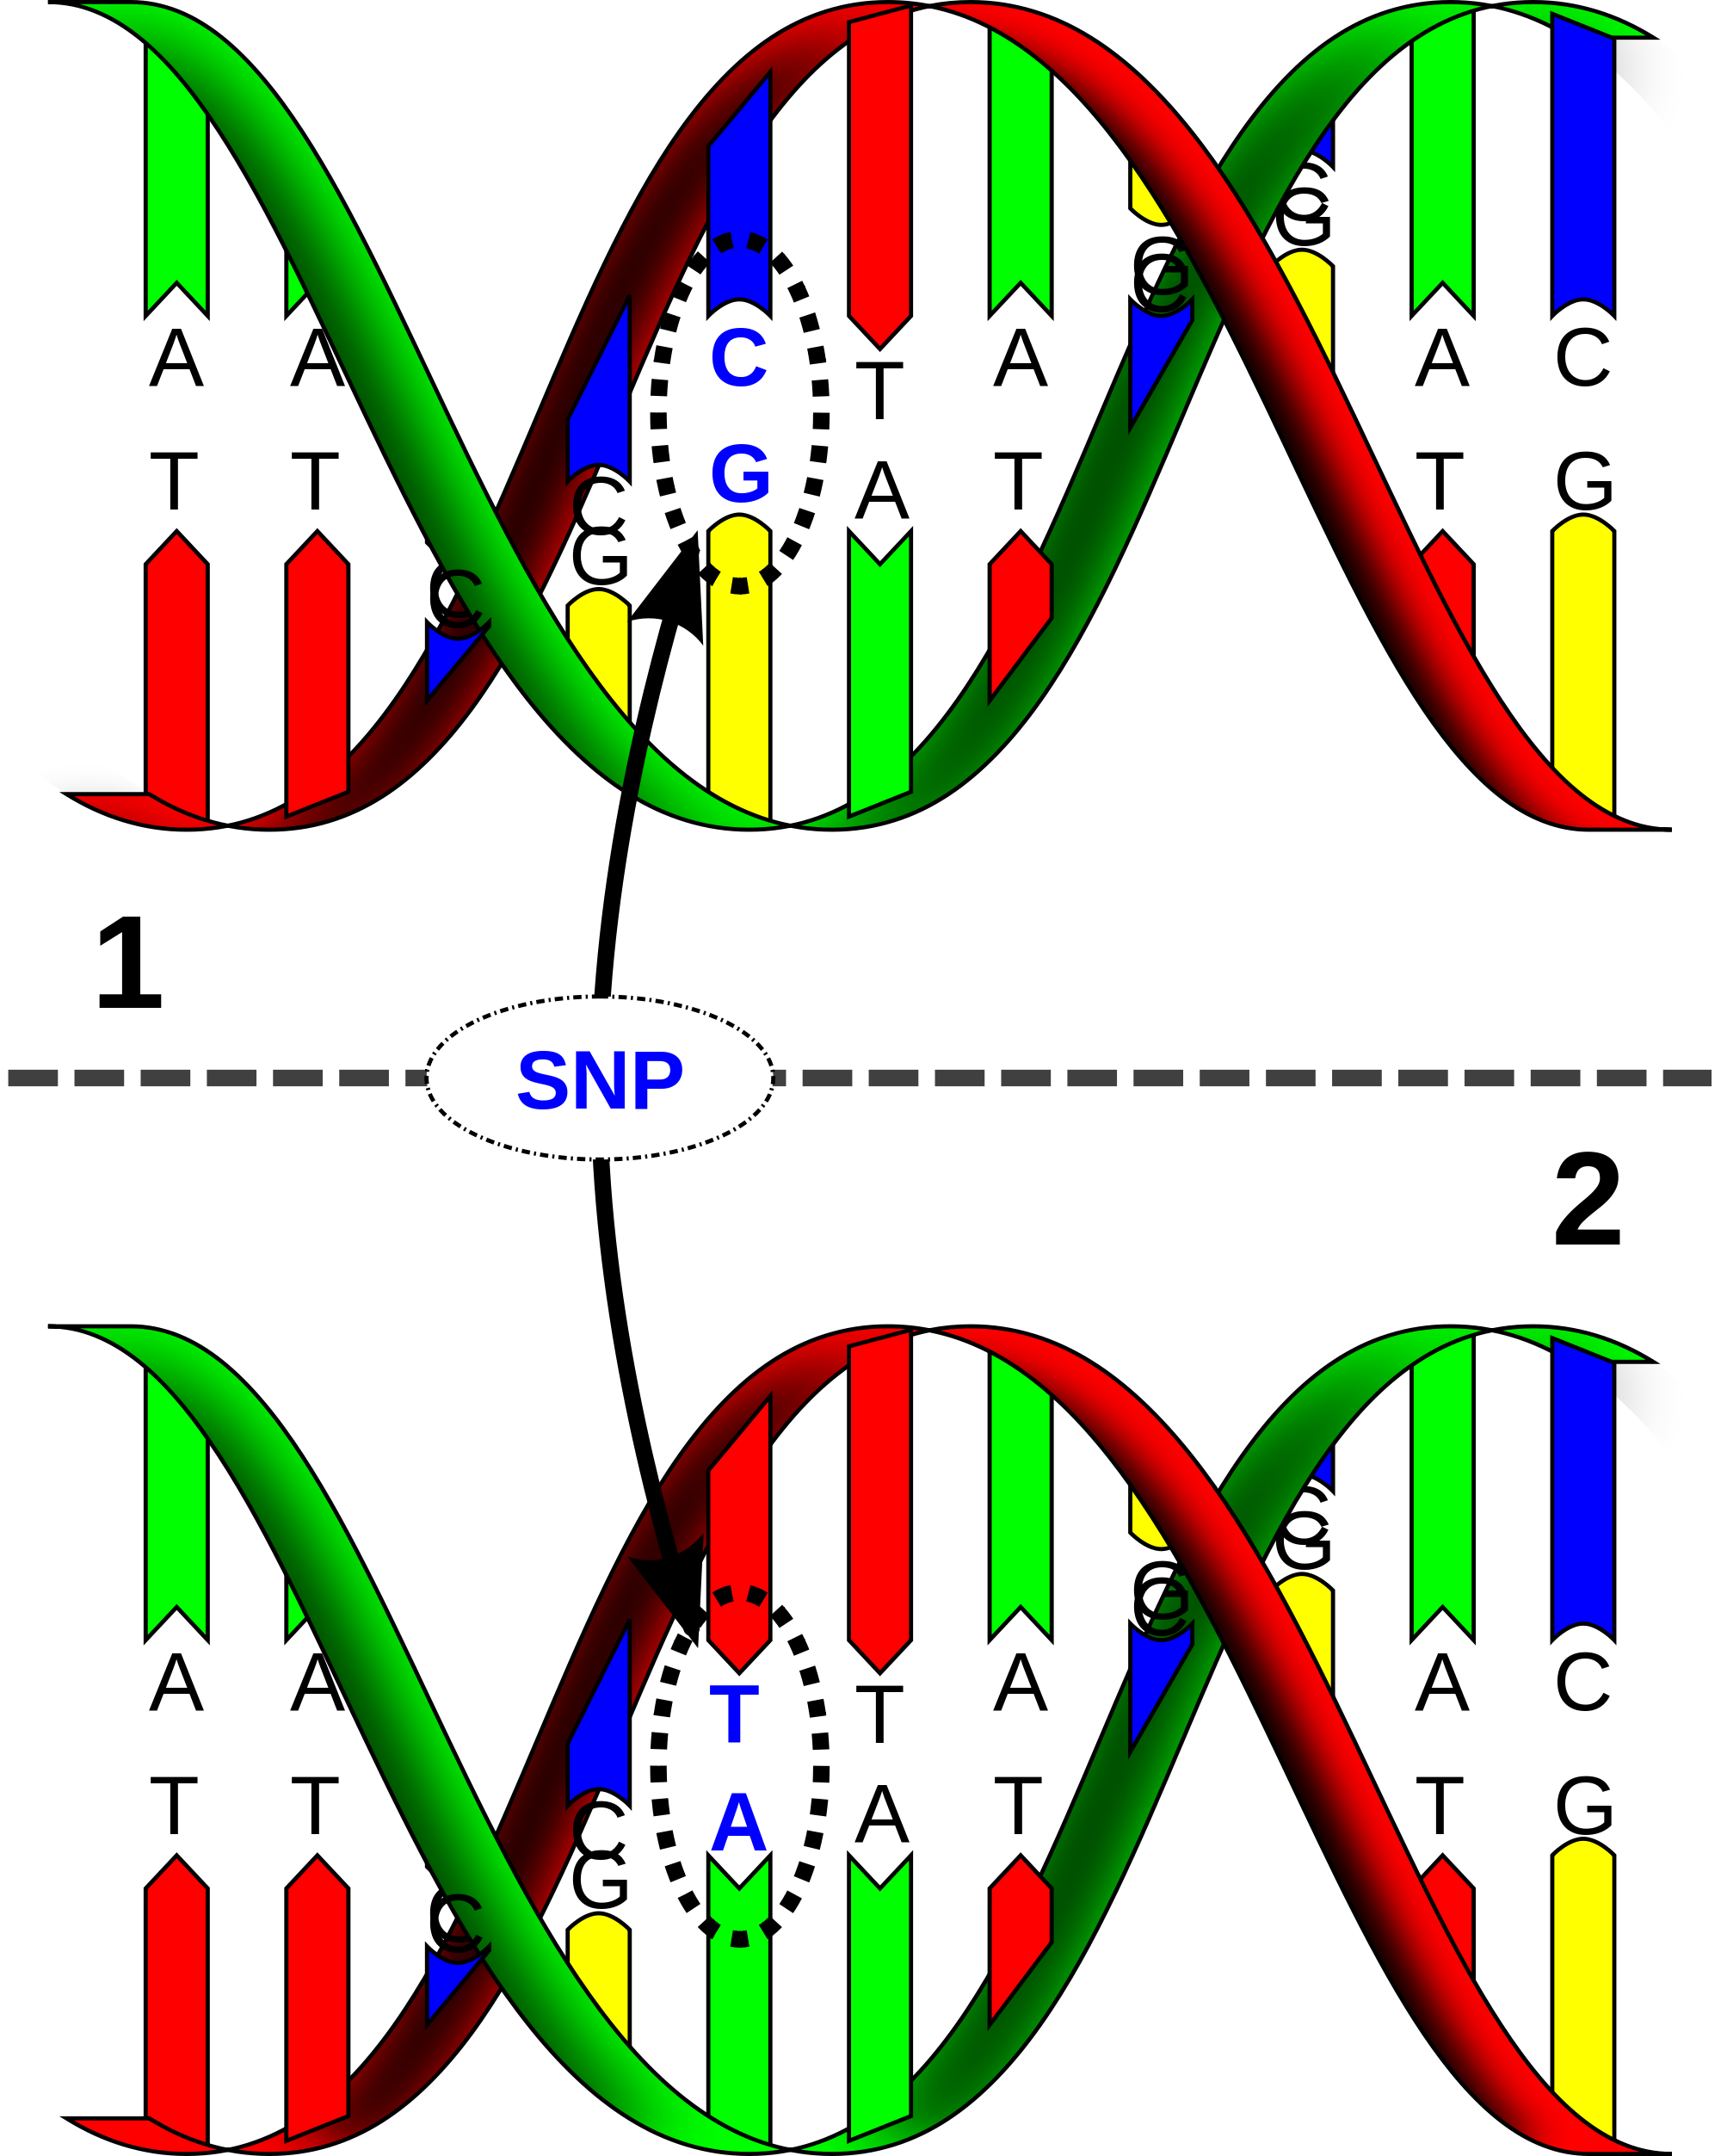
\includegraphics[width=0.8\textwidth]{{{figure/2000px-Dna-SNP.svg}}}
%\vspace{-20pt}
%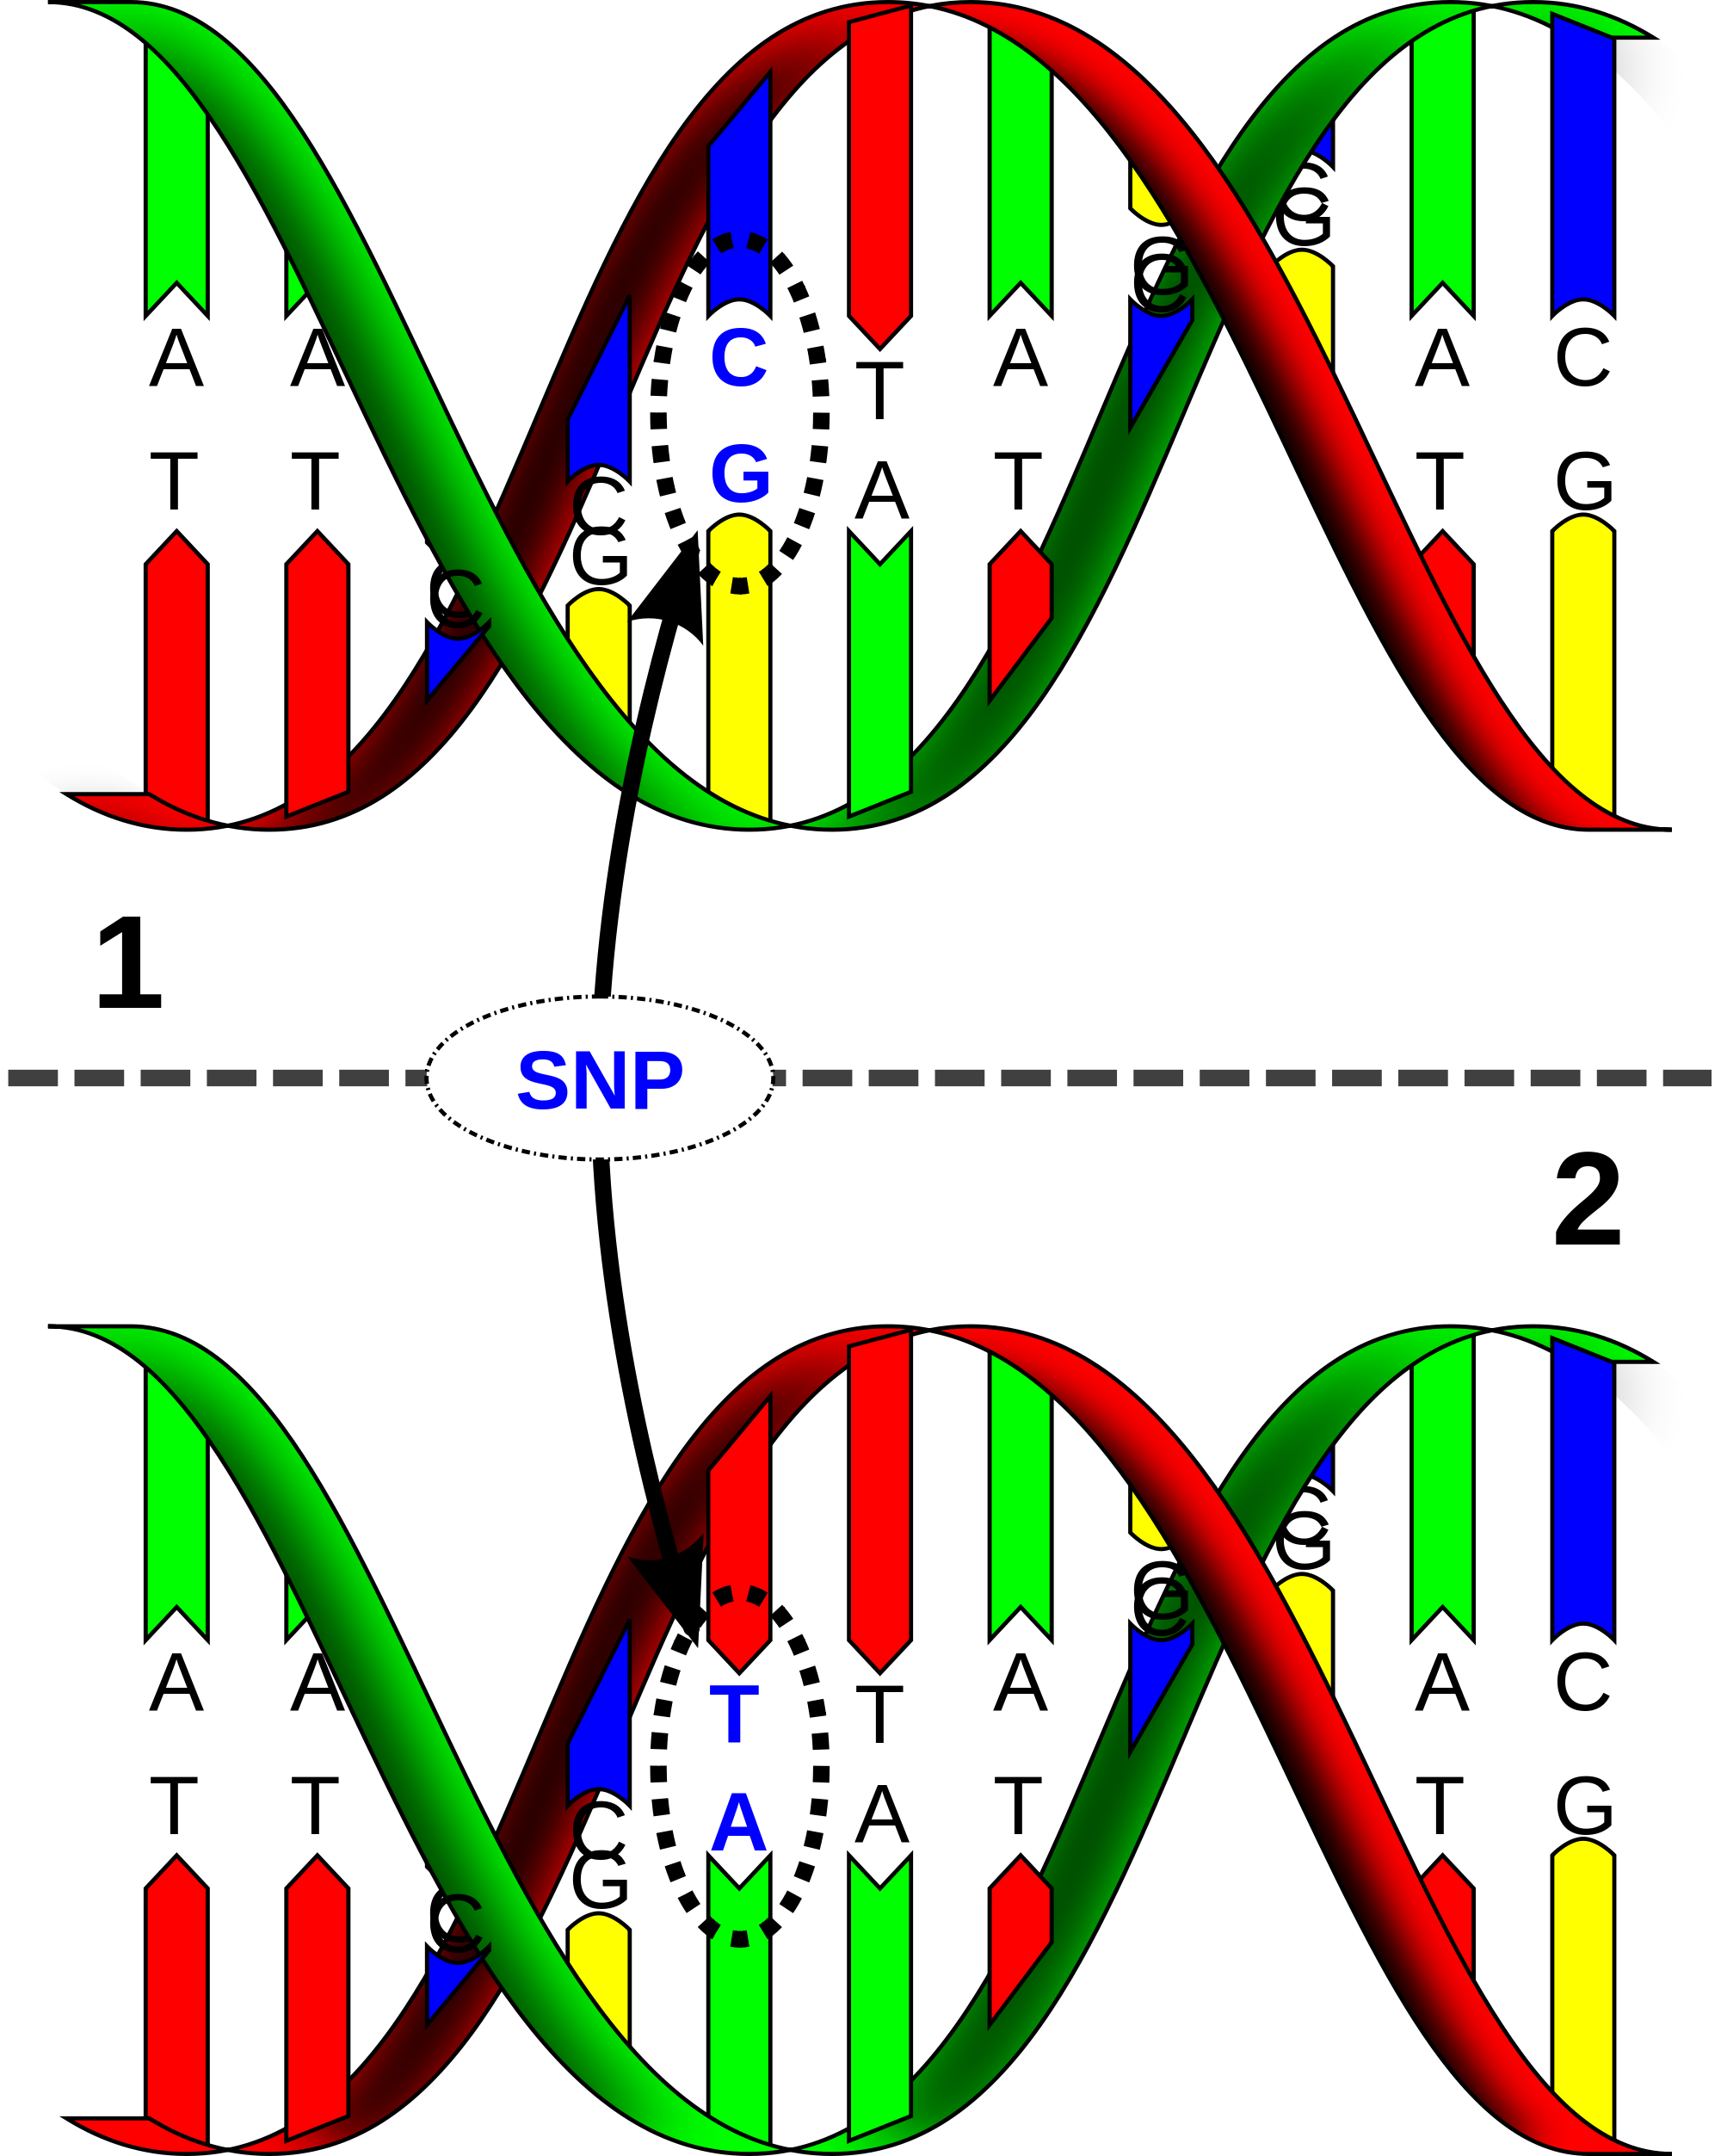
\includegraphics[height=0.6\textheight]{{{figure/2000px-Dna-SNP.svg}}}
%%\caption{ single nucleotide polymorphism \label{fig: 2000px-Dna-SNP.svg}}
%\end{wrapfigure}
%A Single Nucleotide Polymorphism (SNP) is a DNA sequence variation occurring commonly within a population (e.g. 1\%) in which a single nucleotide — A, T, C or G — in the genome (or other shared sequence) differs between members of a biological species or paired chromosomes.
%% For example, two sequenced DNA fragments from different individuals, AAGCCTA to AAGCTTA, contain a difference in a single nucleotide. In this case we say that there are two alleles. Almost all common SNPs have only two alleles. The genomic distribution of SNPs is not homogenous; SNPs occur in non-coding regions more frequently than in coding regions or, in general, where natural selection is acting and 'fixing' the allele (eliminating other variants) of the SNP that constitutes the most favorable genetic adaptation.[1] Other factors, like genetic recombination and mutation rate, can also determine SNP density.[2]
%
%}
%
%%
%%%%%%%%%%%%%%%%%%%%%%%%%%%%%%%%%%%%%%%%%%
%%%2
%%\frame{\frametitle{Introduction to GWAS}
%%\framesubtitle{A simple flowchart}
%%\begin{figure}
%%\vspace{-10pt}
%%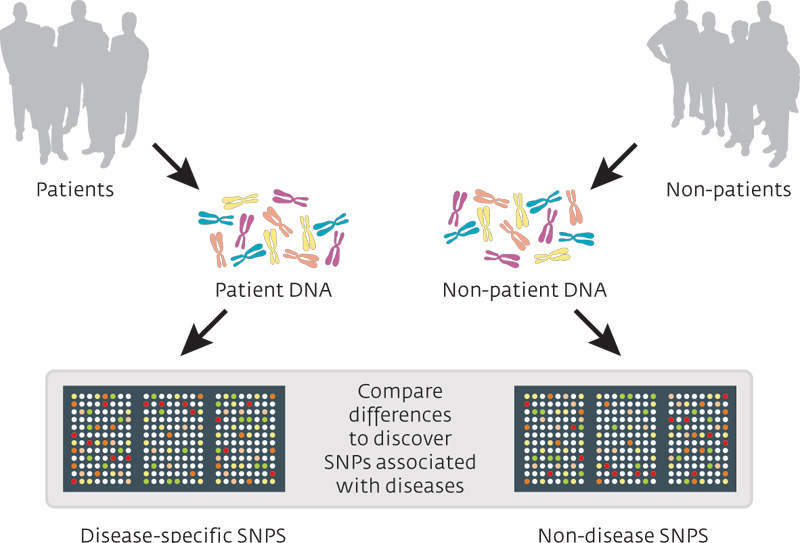
\includegraphics[height=0.6\textheight]{{{figure/gwas_SNPs_casecontrol}}}
%%%\caption{ single nucleotide polymorphism \label{fig: 2000px-Dna-SNP.svg}}
%%\end{figure}
%%
%%}
%%%%%%%%%%%%%%%%%%%%%%%%%%%%%%%%%%%%%%%%%
%%3
%\frame{\frametitle{Introduction to GWAS}
%\framesubtitle{A flowchart of GWAS}
%\begin{figure}
%\vspace{-10pt}
%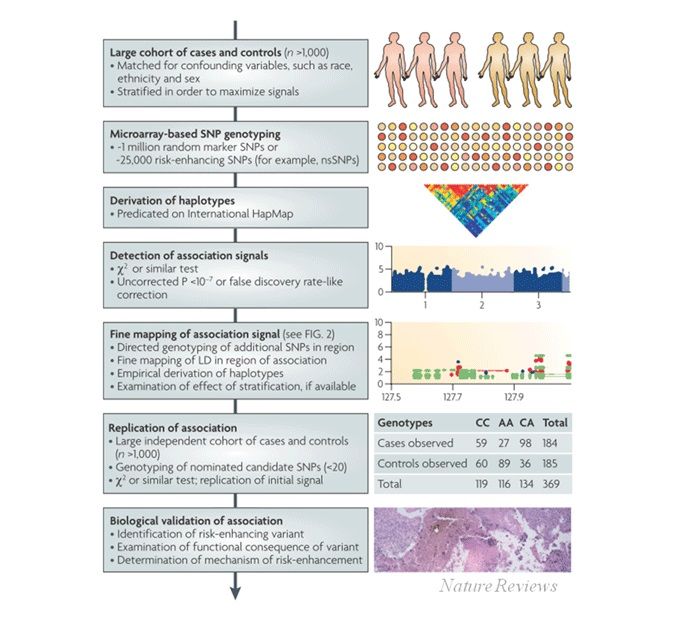
\includegraphics[height=0.8\textheight]{{{figure/gwas_flowchart}}}
%%\caption{ single nucleotide polymorphism \label{fig: 2000px-Dna-SNP.svg}}
%\end{figure}
%
%}
% 
%%%%%%%%%%%%%%%%%%%%%%%%%%%%%%%%%%%%%%%%%
%%4
%\frame{\frametitle{Introduction to GWAS}
%\framesubtitle{How does GWAS result look like?}
%\begin{figure}
%\vspace{-5pt}
%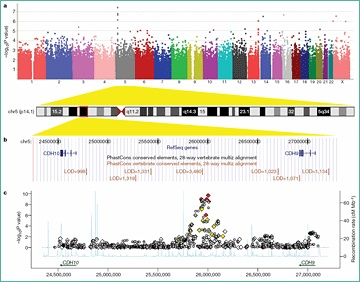
\includegraphics[height=0.7\textheight]{{{figure/GWAS_top10}}}
%\caption{ Common genetic variants on 5p14.1 associate with autism spectrum disorders \cite{Wang2009}}
%\end{figure}
%
%}
%
%%%%%%%%%%%%%%%%%%%%%%%%%%%%%%%%%%%%%%%%%
%%4.5
%\frame{\frametitle{Introduction to GWAS}
%\framesubtitle{GWAS Catalog}
%\begin{figure}
%\vspace{-5pt}
%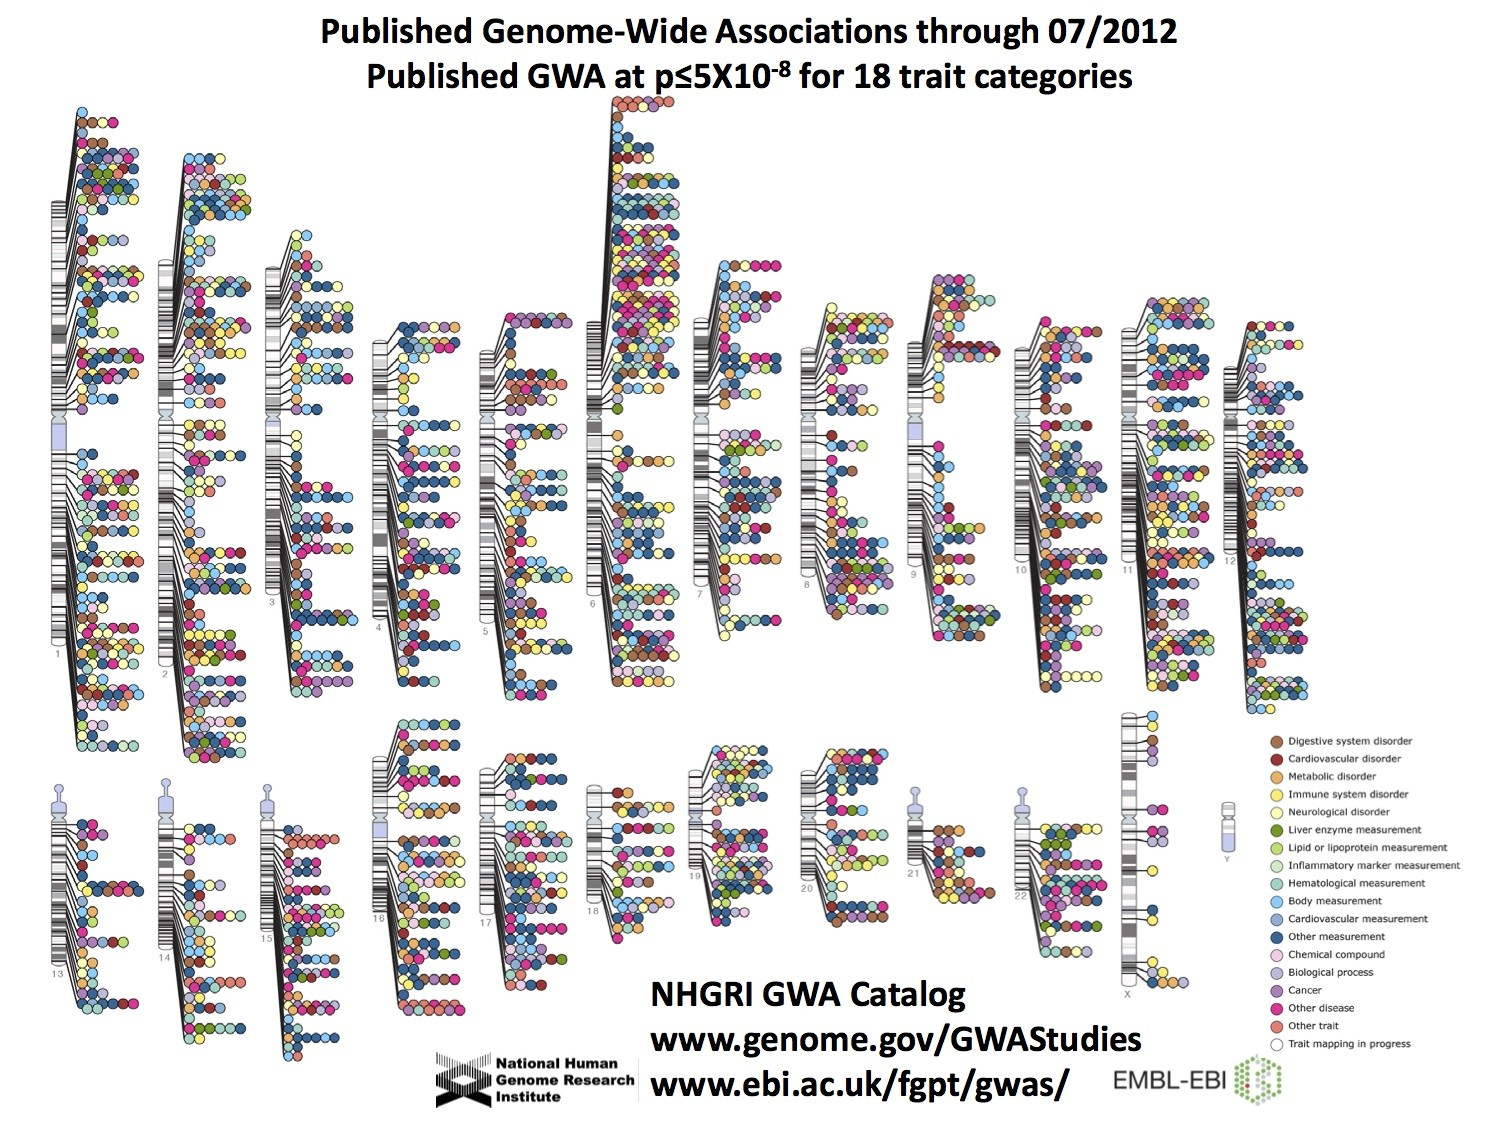
\includegraphics[height=0.7\textheight]{{{figure/2012_GWAS_catalog}}}
%\caption{ Published GWAS results for 18 trait categories}
%\end{figure}
%
%}
%
%\frame{\frametitle{Introduction to GWAS}
%\framesubtitle{GWAS contribute to personalized medicine}
%\begin{figure}
%\vspace{-5pt}
%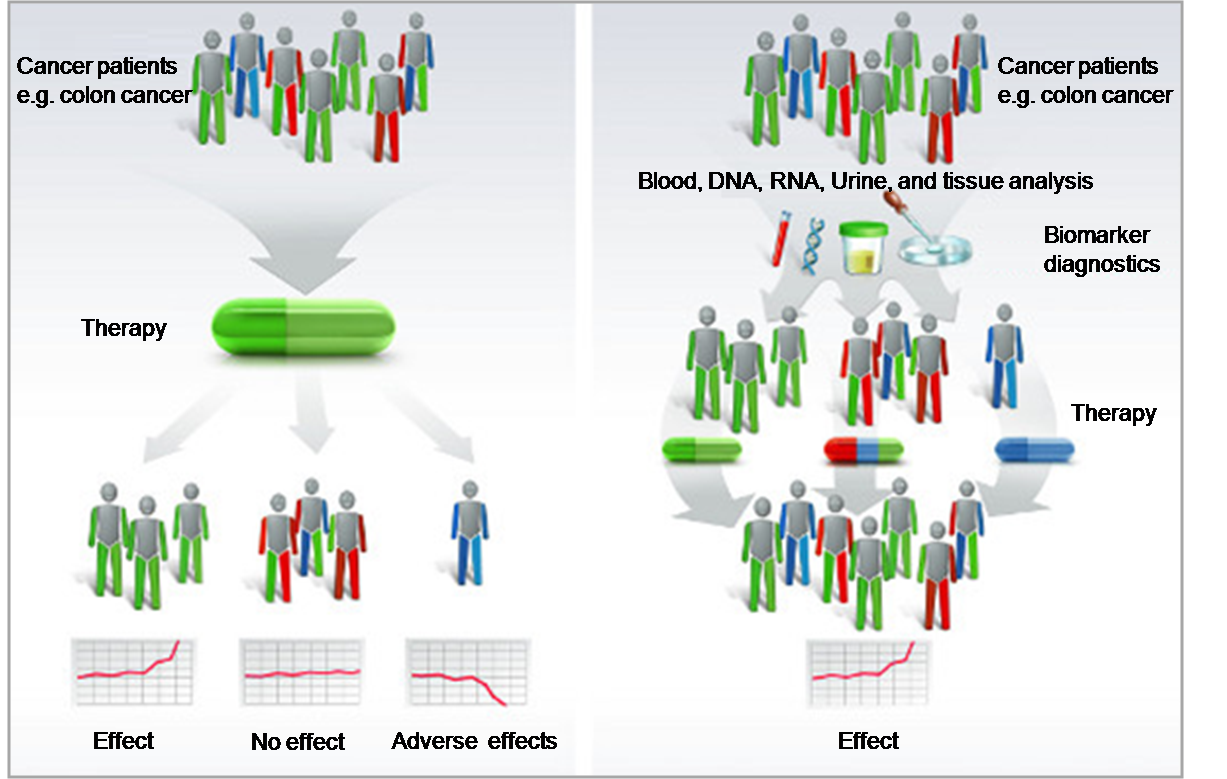
\includegraphics[height=0.7\textheight]{{{figure/Translational_medicine}}}
%\caption{ GWAS contribute to precision medicine}
%\end{figure}
%
%}
%
%%%%%%%%%%%%%%%%%%%%%%%%%%%%%%%%%%%%%%%%%
%%5
%\frame{\frametitle{Introduction to GWAS}
%\framesubtitle{Common variants and rare variants}
%\scriptsize
%\begin{figure}
%\vspace{-5pt}
%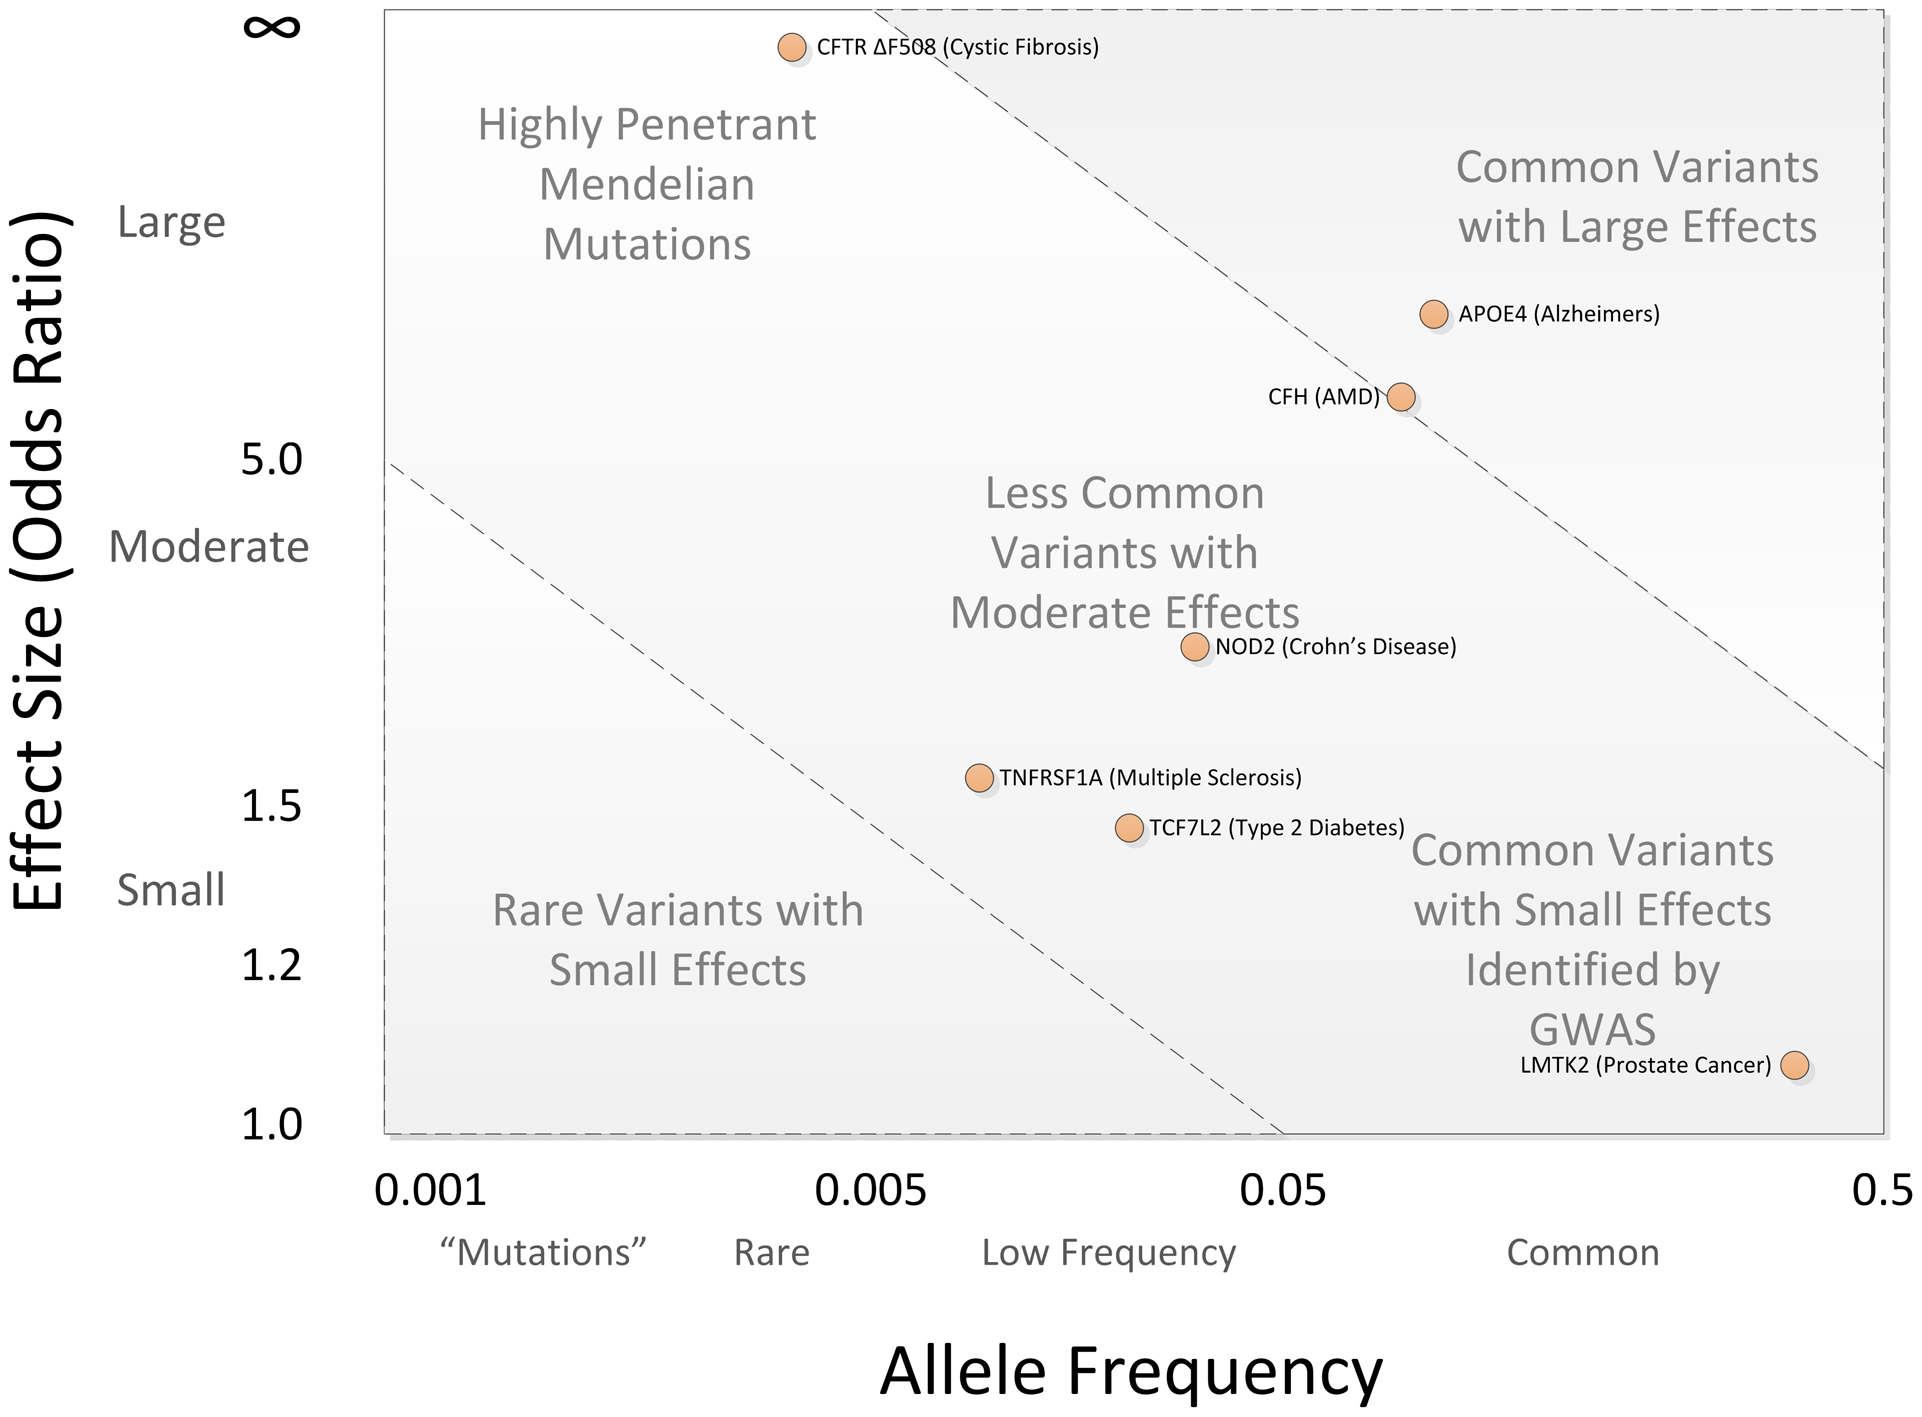
\includegraphics[height=0.7\textheight]{{{figure/GWAS_Disease_allele_effects}}}
%\caption{ effect size of Single Nucleotide Variant \cite{Bush2012} }
%\end{figure}
%
%}  
%
%%%%%%%%%%%%%%%%%%%%%%%%%%%%%%%%%%%%%%%%%%%%%%%%%%%%
%%%%%%%%%%%%%%%%%%%%%%%%%%%%%%%%%%%%%%%%%%%%%%%%%%%%
%%%%%%%%%%%%%%%%%%%%%%%%%%%%%%%%%%%%%%%%%%%%%%%%%%%%
%%%%%%%%%%%%%%%%%%%%%%%%%%%%%%%%%%%%%%%%%%%%%%%%%%%%
%\subsection{SNP-set based association tests}
%%%%%%%%%%%%%%%%%%%%%%%%%%%%%%%%%%%%%%%%%%%%%%%%%%%%
%\frame{
%\frametitle{Table of Contents}
%%\begin{itemize}
%%\item Introduction to GWAS
%%\item Gene-based association test
%%\item Longitudinal data analysis strategy
%%\item Gene-set/Pathway based association test
%%\end{itemize}
%\small
%\tableofcontents[currentsection,currentsubsection]
%}
%%%%%%%%%%%%%%%%%%%%%%%%%%%%%%%%%%%%%%%%%%%%%
%%1
%\frame{\frametitle{single-SNP based association tests}
%\framesubtitle{the classical method}
%\footnotesize
%For individual $i$ with SNP $j$ coded as $x_{ij}$ ($x_{ij} = 0, 1, 2$ representing copies of minor alleles) and a vector of covariates $\varphi_i$, 
%\[g(\mu_i)=\beta_0 + x_{ij}\beta_j + z_i \varphi_i, \]
%% where $g(\mu_i)$ is a link function in Genaralized Linear Model (GLM) to link types of outcome to the linear combination of predictors.\\\
%
%However, this method suffers from at least two disadvantages: \\
%1), it will generate millions of tests thus increase the multiple test error correction burden; \\
%2), the coefficient estimate of SNP $j$ will become unstable or even the estimation algorithm cannot converge when SNP minor allele frequency (MAF) becomes smaller, e.g. MAF $ < 0.01$. 
%
%
%%\begin{itemize}
%%\item Question to answer: does this particular SNP $j$ significantly affect the prediction of $g(\mu_i)$ when the other covariates presented in the model?
%%\item $H_0: \beta_j=0$,
%%$H_1: \beta_j\ne0$
%%\item $TS=\frac{\hat{\beta}_j}{\hat{se}(\hat{\beta}_j)}\sim t_{n-3}$, reject $H_0$ if $|TS|>t_{n-3,1-\alpha/2}$
%%\item This is a {\bf partial test} because $\hat{\beta}_j$ depends on all of the other predictors $x_i$, for $i\ne j$, that are in the model. Thus, this is a test of the contribution of $x_j$ given other predictors in the model.
%%\end{itemize}
%
%}  
%
%
%%%%%%%%%%%%%%%%%%%%%%%%%%%%%%%%%%%%%%%%%%%%%
%%2
%\frame[allowframebreaks]{
%\frametitle{SNP-set based association tests}
%%\framesubtitle{the improved strategy against low MAF SNVs}
%\framesubtitle{A brief review}
%\footnotesize
%By pooling multiple low MAF SNVs together, the SNP-set based association test can detect the signal(s) from a region (such as a gene) instead of from a single SNV.\\
%\begin{figure}
%\vspace{-5pt}
%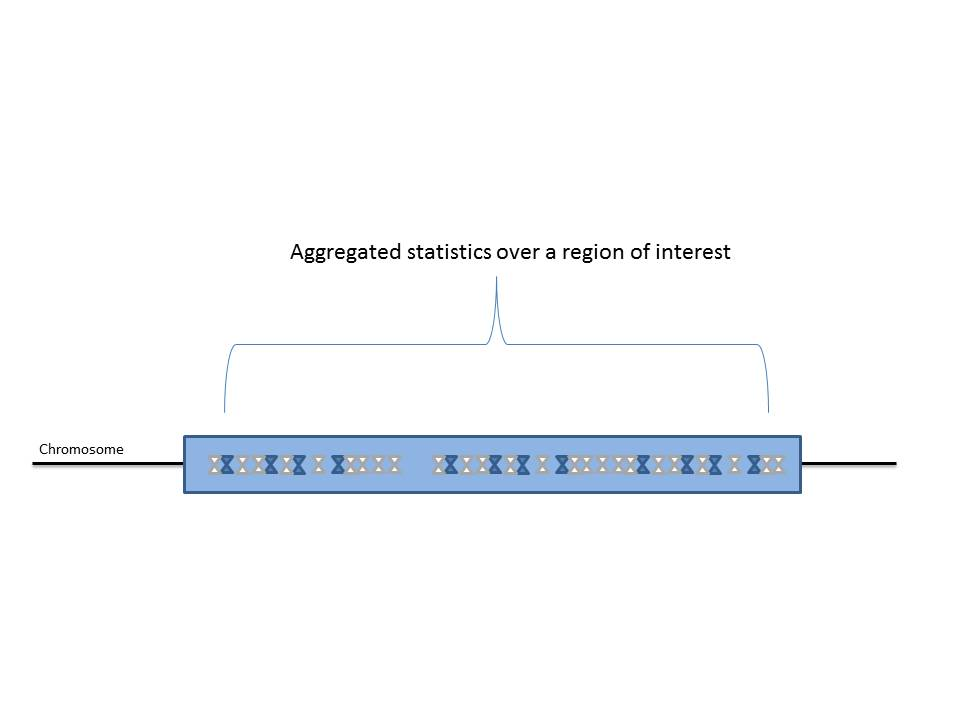
\includegraphics[height=0.7\textheight]{{{figure/SNP-set_assoc_test_demo}}}
%%\caption{ effect size of Single Nucleotide Variant \cite{Bush2012} }
%\end{figure}
%%%%
%Major categories of SNP-set based association tests:
%\begin{small}
%
%\begin{itemize}
%\item the so-called "burden test", which used MAF based weighting scheme to combine the sum statistics from multiple SNVs in a region \cite{Li2008,Madsen2009};
%%%%%%%%%%%%%%%
%\item the variance-component test, which includes SKAT, C-alpha, SSU, etc \cite{Pan2009,Neale2011,Wu2011}. 
%
%\item the Lasso and group-penalized regression based methods \cite{Zhou2010,Kim2014}.
%
%
%\item the functional linear model and functional principal component analysis based methods \cite{Luo2012,Luo2012a,Luo2011,Fan2013}.
%
%\item the adaptive test combines statistics of burden test and variance-component test, such as SKAT-O, aSum, aSSU, aScore, an exponential combination (EC) framework for set-based association tests, a robust and powerful
%test using Fisher's method to combine linear and quadratic statistics, a unified mixed-effect model, etc \cite{Han2010,Pan2011,Lee2012,Lee2012a,Chen2012,Derkach2013,Sun2013}.
%\end{itemize}
%
%\end{small}
%
%
%}
%
%%%%%%%%%%%%%%%%%%%%%%%%%%%%%%%%%%%%%%%%%%%%%%%%%%%%
%%%%%%%%%%%%%%%%%%%%%%%%%%%%%%%%%%%%%%%%%%%%%%%%%%%%
%%%%%%%%%%%%%%%%%%%%%%%%%%%%%%%%%%%%%%%%%%%%%%%%%%%%
%%%%%%%%%%%%%%%%%%%%%%%%%%%%%%%%%%%%%%%%%%%%%%%%%%%%
%\subsection{Longitudinal data analysis strategy in GWAS}
%%%%%%%%%%%%%%%%%%%%%%%%%%%%%%%%%%%%%%%%%%%%%%%%%%%%
%\frame{
%\frametitle{Table of Contents}
%\small
%\tableofcontents[currentsection,currentsubsection]
%}
%%%%%%%%%%%%%%%%%%%%%%%%%%%%%%%%%%%%%%%%%%%%%
%%1
%\frame{
%\frametitle{How do longitudinal data look like?}
%%\framesubtitle{the vantage method}
% \begin{tiny}
%\begin{figure}
%\centering
%\vspace{-5pt}
%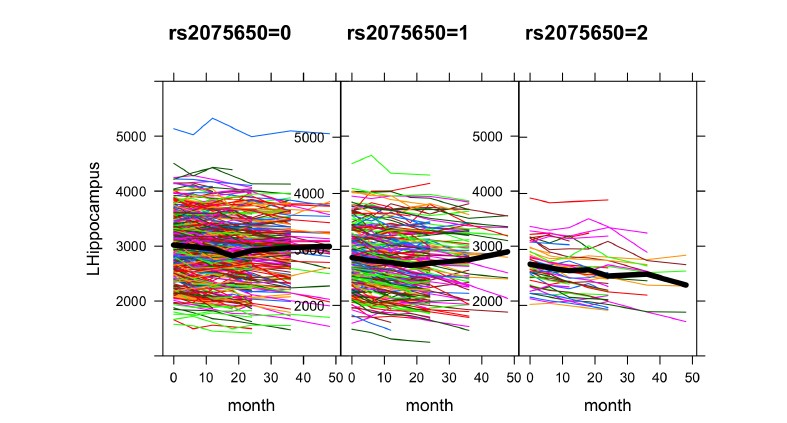
\includegraphics[height=0.6\textheight]{{{figure/longi_look}}}
%\vspace{-10pt}
%
%{ \caption{  Trajectories of phenotype left hippocampus volume over time (in months) in three allele groups of SNP rs2075650 \cite{Xu2014} } }
%
%\end{figure}
%\end{tiny}
%}
%%%%
%% In Amazon, longitudinal data can be the a consumer's expenditure over years, a packaging unit's error rate over months, etc.
%%%%
%
%%2
%\frame[allowframebreaks]{
%\frametitle{Why longitudinal?}
%%\framesubtitle{the vantage method}
%\footnotesize
%In a cross-sectional study ($n_i = 1$) we are restricted to the model
%$$Y_{i1} = \beta_C x_{i1} + \epsilon_{i1}, \quad i = 1,\ldots,m, $$
%where $\beta_C$ represents the difference in average $Y$ across two sub-populations (samples) which differ by one unit in $x$. With repeated measurements, the above linear model can be extended to
%$$ Y_{ij} = \beta_C x_{i1} + \beta_L ( x_{ij} - x_{i1} ) + \epsilon_{ij}, \quad i = 1, \ldots, m; \ j = 1, \ldots, n_i $$
%\cite{WARE1990}. 
%%Now $\beta_C$ still represents the cross-sectional difference while $\beta_L$ is interpreted as the expected change in $Y$ over time per unit change in $x$ for a given subject. The basic of inference about $\beta_C$ is a comparison of individuals with a particular value of $x$ to other individuals with a different value of $x$. In contrast, the parameter estimation of $\beta_L$ is by comparing a person's responses at two times, assuming $x$ changes with time.
%
%Based on above formula, we can more obviously explain the merits of longitudinal studies over cross-sectional studies. 
%\begin{enumerate}
%\item Longitudinal studies allow us to estimate both the cross-sectional difference ($\beta_C$) and the rate change over time ($\beta_L$).
%\item Even when $\beta_C = \beta_L$, longitudinal studies tend to be more powerful than cross-sectional studies. This is due to the fact that in longitudinal studies, each person can be thought of serving as his/her own control. 
%%For most outcomes $Y$, there is considerable variability across individuals due to the influence of unmeasured characteristics such as genetic make-up, environmental exposures, personal behaviors/habits, and so forth. While these things tend to persist over time for the same individual, their influences are canceled in the estimation of the $\beta_L$ or equivalently here the $\beta_C$, and thus lead to more accurate estimate (smaller variance).
%%%%%%%%
%\item Another merit of the longitudinal study is its ability to distinguish the between-subject variation and within-subject variation.
%
%%the degree of variation in $Y$ across time for one subject from the variation in $Y$ across subjects. 
%%With repeated measurements, we can borrow strength across time for the same person of interest as well as across people. If there is little variation across subjects, one subject's estimate can rely on data from others as in the cross-sectional case. However, if the variation across people is large, we might prefer to use more data for the same individual across time.
%\item With longitudinal studies, we can estimate a person's current and future outcome (behavior trend). 
%\end{enumerate}
%
%
%\framebreak
%\textbf{Longitudinal study in GWAS}\\
%A recent study by Xu et al \cite{Xu2014} demonstrates the power gain from longitudinal data analysis over traditional cross-sectional data analysis used in GWAS.
%\begin{figure}
%\centering
%\vspace{-5pt}
%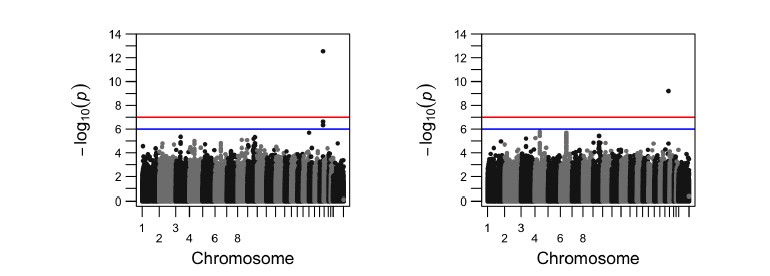
\includegraphics[width=0.8\textwidth]{{{figure/longi_advantage1}}}
%\vspace{-10pt}
%
% \caption{  Comparison of the Manhattan plots for genome-wide p-values for phenotype left hippocampus volume from longitudinal analysis (left) and from cross-sectional analysis (right) \cite{Xu2014} } 
%
%\end{figure}
%
%%\begin{figure}
%%\centering
%%\vspace{-5pt}
%%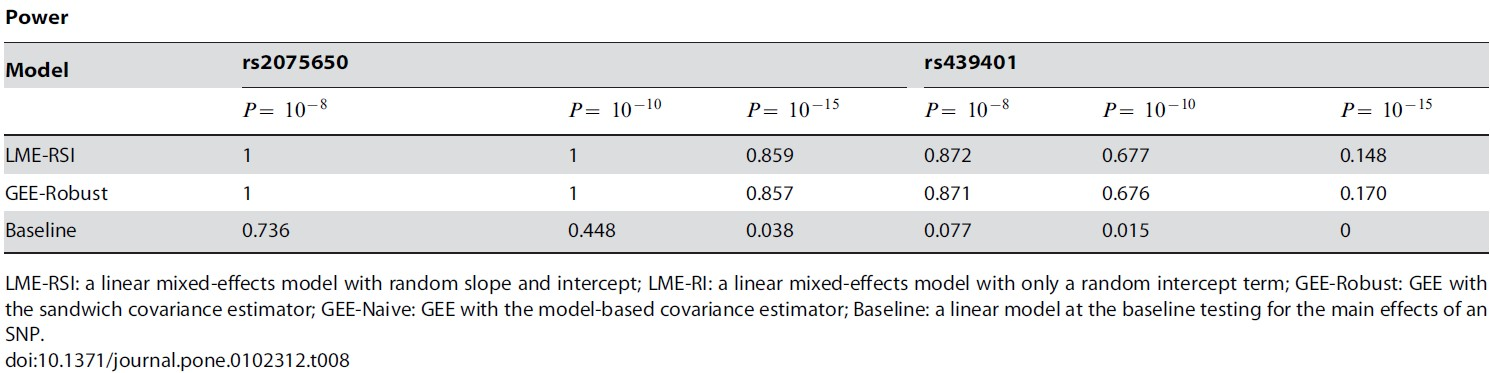
\includegraphics[width=1\textwidth]{{{figure/longi_advantage5}}}
%%\vspace{-10pt}
%%
%% \caption{  Simulation results at significance level P with different methods \cite{Xu2014} } 
%%
%%\end{figure}
%
%}
%
%%3
%\frame[allowframebreaks]{
%\frametitle{A brief review of major longitudinal data analysis methods}
%%\framesubtitle{the vantage method}
%Major categories of longitudinal data analysis methods:
%\begin{scriptsize}
%
%\begin{itemize}
%\item random effect models\\
%Random effect model is a two-stage models, which treat probability distributions for the response vectors of different individuals as a single family and the random-effects parameters which hold the same for the same individual as another distribution \cite{laird1982random}.
%%%%%%%%%%%%%%%
%%\framebreak
%\item marginal effect models\\
%Marginal effect model is an extension to
%quasi-likelihood method. Rather than giving subject-specific(SS) estimates as in random effect models, marginal effect models by Generalized Estimating Equation (GEE) give population-averaged (PA) estimates.
% 
%%\framebreak
%\item transitional (Markov) models \\
%The transitional (Markov) model, describes the conditional distribution of each response $y_{ij}$ as an explicit function of first $q$ prior observations $y_{ij-1},\dots,y_{ij-q}$ from history response vector: $H_{ij} = \{ y_{ik}, k = 1,\dots,j - 1\}$ and covariates $x_{ij}$. The integer $q$ is referred as the order of the Markov models.
%
%
%\end{itemize}
%\end{scriptsize}
%
%}
%%
%%
%%%%%%%%%%%%%%%%%%%%%%%%%%%%%%%%%%%%%%%%%%%%%%%%%%%%%
%%%%%%%%%%%%%%%%%%%%%%%%%%%%%%%%%%%%%%%%%%%%%%%%%%%%%
%%%%%%%%%%%%%%%%%%%%%%%%%%%%%%%%%%%%%%%%%%%%%%%%%%%%%
%%%%%%%%%%%%%%%%%%%%%%%%%%%%%%%%%%%%%%%%%%%%%%%%%%%%%
%%\subsection{Gene-Set/Pathway based association tests in GWAS}
%%%%%%%%%%%%%%%%%%%%%%%%%%%%%%%%%%%%%%%%%%%%%%%%%%%%%
%%\frame{
%%\frametitle{Table of Contents}
%%\tableofcontents[currentsection,currentsubsection]
%%}
%%%%%%%%%%%%%%%%%%%%%%%%%%%%%%%%%%%%%%%%%%%%%%
%%%1
%%\frame{
%%\scriptsize
%%\frametitle{A big picture}
%%%\framesubtitle{the vantage method}
%%\begin{figure}
%%\vspace{-5pt}
%%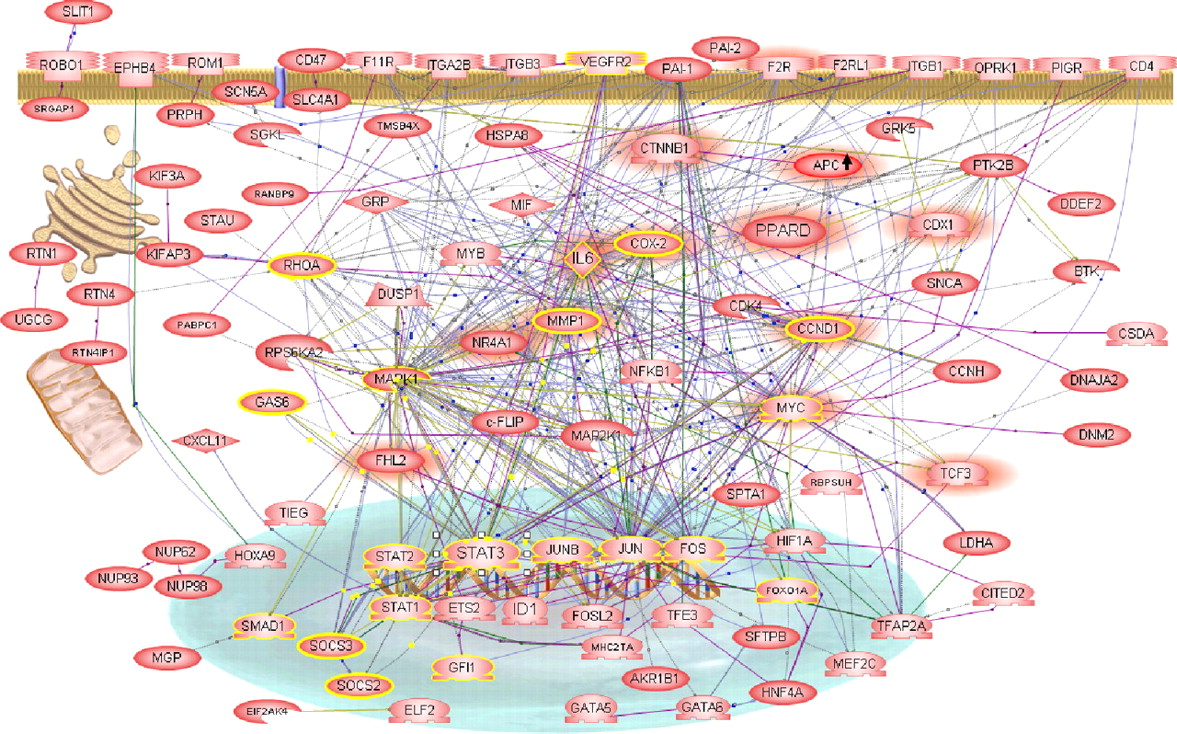
\includegraphics[height=0.5\textheight]{{{figure/gene_network1}}}
%%%\caption{ single nucleotide polymorphism \label{fig: 2000px-Dna-SNP.svg}}
%%\end{figure}
%%\textbf{The advantage of using Gene-Set/Pathway based association test in GWAS:}
%%\begin{itemize}
%%\item it utilizes the information of biological pathway to help localize the association signal(s) from close related genes
%%\item it further aggregates multiple Genes/RVs against testing each Gene/RV separately, which will boost the statistical power
%%\end{itemize}
%%
%%
%%%Extending the gene-based association test to sets of multiple related genes could return more biological meaningful inference, as in vivo, there are usually multiple genes working together to fulfill a biological function, analyzing "co-workers" genes together with phenotype tends to identify those signals hidden from or attenuated in single-gene based tests \cite{BloodPressureGenome-WideAssociationStudies2011,Hirschhorn2009,Zhong2010,Wang2010}. Complex disease are known to have a combination of genetic factors in addition to environmental, lifestyle factors, and their interactions \cite{Hirschhorn2005,McCarthy2008}. Thus by investigating into the sets of genes, more evidence could be extracted as risk altering factors contributing to a specific disease. The other reason for considering pathway-based association test is similar to the consideration for gene-based association test: aggregating multiple Genes/RVs against testing each Gene/RV separately will boost the statistical power. One convincing evidence is from The Cancer Genome Atlas (TCGA: http://cancergenome.nih.gov/) for doing tumor sequencing studies. While only few oncogenes (e.g. TP53, EGFR) harbor many mutations, most others harbor few mutations in a tumor-dependent manner. Single gene-based association test thus still suffer from low aggregated mutation frequency, whereas collectively, they have a much higher aggregated mutation frequency in a gene-set/pathway. Therefore, for some disease such as cancer to investigate its association with somatic mutations, a gene-set/pathway analysis by aggregating information across genes will boost the statistical power, and is thus preferred.
%%}
%%
%%
%%%%2
%%%\frame{
%%%\frametitle{the advantage of using Gene-Set/Pathway based association test in GWAS}
%%%%\framesubtitle{the vantage method}
%%%\begin{itemize}
%%%\item it utilizes the information of biological pathway to help localize the association signal from close related genes
%%%\item it aggregates multiple Genes/RVs against testing each Gene/RV separately, which will boost the statistical power
%%%\end{itemize}
%%%
%%%}
%%
%%%3
%%\frame{
%%\scriptsize
%%\frametitle{Types of Gene-Set/Pathway based association test in GWAS}
%%%\framesubtitle{the vantage method}
%%\scriptsize
%%\begin{figure}
%%\vspace{-5pt}
%%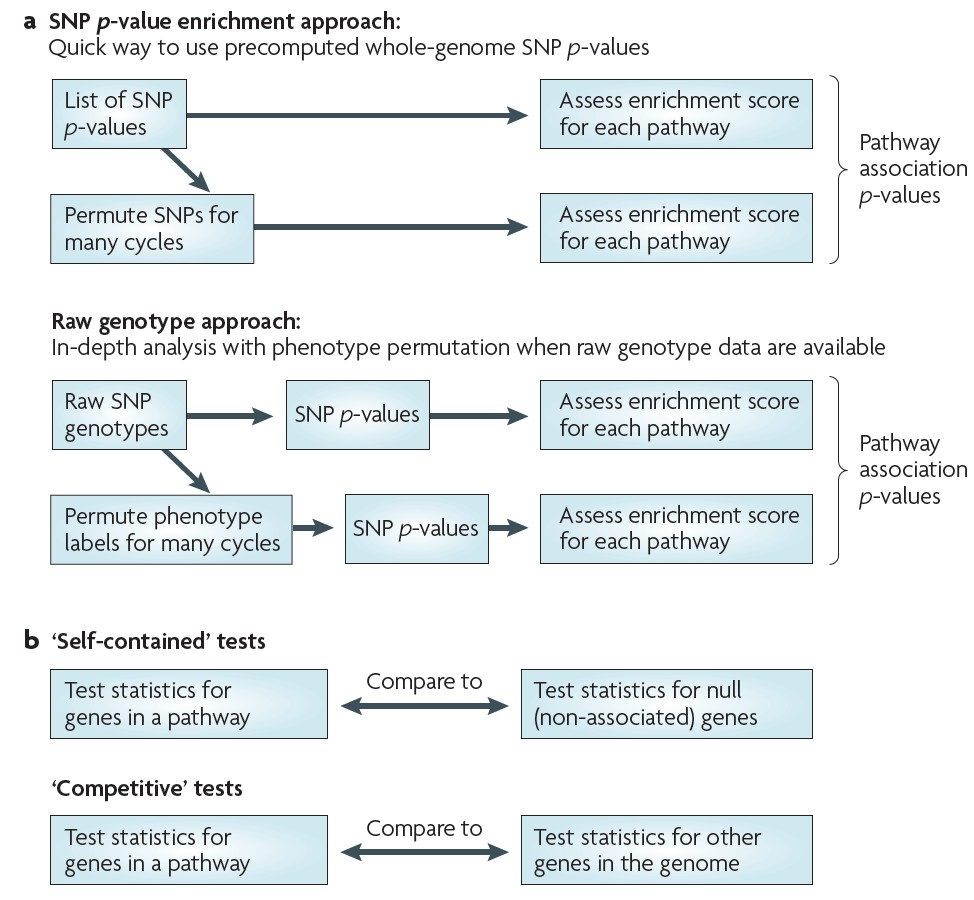
\includegraphics[height=0.7\textheight]{{{figure/pathwayTests_definition}}}
%%\caption{ Types of pathway association method \cite{Wang2010} }
%%\end{figure}
%%
%%
%%
%%
%%}
%%
%%%4
%%\frame[allowframebreaks]{
%%\frametitle{A brief review of current Gene-Set/Pathway based association tests in GWAS}
%%%\framesubtitle{the vantage method}
%%\footnotesize
%%\begin{itemize}
%%\item GSEA modification in GWAS; GSEA-SNP;i-GSEA4GWAS
%%\item modification of Fishers method for combing SNP P-values for gene-level or gene-set-level association
%%\item gene set ridge regression in association studies (GRASS)
%%\item association list go annotator (ALIGATOR), which is a 'p-value enrichment approach' requiring only pre-computed SNP p-values, uses Fisher's exact test on SNP with minimum p-value for the gene-level association
%%\item the SNP ratio test (SRT),tests the ratio of significant SNPs in a pathway and compute the empirical p-value based on permutation
%%\item supervised principal component analysis with a
%%Gumbel extreme value mixture distribution as test statistic distribution and simulation-based
%%standardization procedure for pathway size
%%%\item the Gene-loci Set Analysis (GLOSSI), at first uses the Cochran-Armitage trend test at
%%single-marker level assuming an additive SNP effect, then uses Fisher's combination test to
%%combine individual p-values of markers and corrected by Brown's approximation to better
%%control type I error
%%%\item an adaptive rank truncated product (ARTP) statistic and permutation-based p-value adjustment to combine marker-level p-values to derive gene-level significance level and/or combine gene-level p-values to derive pathway-level significance level
%%\end{itemize}
%%
%%}
%%
%%
%%%%%%%%%%%%%%%%%%%%%%%%%%%%%%%%%%%%%%%%%%%%%%%%%%%%%
%%%%%%%%%%%%%%%%%%%%%%%%%%%%%%%%%%%%%%%%%%%%%%%%%%%%%
%%%%%%%%%%%%%%%%%%%%%%%%%%%%%%%%%%%%%%%%%%%%%%%%%%%%%
%%%%%%%%%%%%%%%%%%%%%%%%%%%%%%%%%%%%%%%%%%%%%%%%%%%%%
%%\section{Tentative Journal Articles}
%%%%%%%%%%%%%%%%%%%%%%%%%%%%%%%%%%%%%%%%%%%%%%%%%%%%%
%%\frame{
%%\frametitle{Table of Contents}
%%\small
%%\tableofcontents[currentsection,currentsubsection]
%%}
%%%%%%%%%%%%%%%%%%%%%%%%%%%%%%%%%%%%%%%%%%%%%%
%%%1
%%\frame{
%%\frametitle{Journal Articles}
%%%\framesubtitle{the vantage method}
%%\begin{small}
%%\begin{itemize}
%%\item Aim 1: Data-adaptive SNP-set-based association tests (aSPU) for longitudinal data analysis within GEE framework for \textbf{Common Variants};\\
%%%	\begin{itemize}
%%%	\item (a), for CVs;
%%%	\item (b), for RVs.
%%%	\end{itemize}
%%%\item Aim 1(b): Longitudinal aSPU family tests on Rare Variants
%%%\item Aim 2: Pathway-based longitudinal aSPU family tests: Path-aSPU
%%\item Aim 2: Longitudinal aSPU family tests on \textbf{Rare Variants}
%%%\item Aim 3: Package/software development
%%\item Aim 3: \textbf{Pathway-based} longitudinal aSPU family tests
%%\end{itemize}
%%\end{small}
%%}
%
%%%%%%%%%%%%%%%%%%%%%%%%%%%%%%%%%%%%%%%%%%%%%%%%%%%%%
%%%%%%%%%%%%%%%%%%%%%%%%%%%%%%%%%%%%%%%%%%%%%%%%%%%%%
%%%%%%%%%%%%%%%%%%%%%%%%%%%%%%%%%%%%%%%%%%%%%%%%%%%%%
%%%%%%%%%%%%%%%%%%%%%%%%%%%%%%%%%%%%%%%%%%%%%%%%%%%%%
%%\section{Public Health Significance}
%%%%%%%%%%%%%%%%%%%%%%%%%%%%%%%%%%%%%%%%%%%%%%%%%%%%%
%%\frame{
%%\frametitle{Table of Contents}
%%\small
%%\tableofcontents[currentsection,currentsubsection]
%%}
%%%%%%%%%%%%%%%%%%%%%%%%%%%%%%%%%%%%%%%%%%%%%%
%%%1
%%\frame[allowframebreaks]{
%%\frametitle{Public Health Significance}
%%%\framesubtitle{the vantage method}
%%\begin{scriptsize}
%%
%%\begin{enumerate}
%%\item Due to the \textbf{complexity} in genetics association with phenotype, e.g. specific association effect directions and sizes, a given test favoring one scenario may or may not perform well in other scenarios \cite{Pan2009,Derkach2013,pan2014powerful,Sun2013}. In other words, there is \textbf{no single test} the most powerful among all testing scenarios.\\\
%%
%%Therefore, a few data-adaptive tests were developed as an ad hoc strategy, e.g. some tests tried to combine the advantage of burden test and variance-component test; some other tests tried to use a set of pre-determined weights for individual RVs. \\\
%%
%%Compared to the previous limited sense data-adaptive tests, our proposed method will be more extensive and generalized in \textbf{data adaptability}. The new tests will provide a relative high power in almost all data scenarios;
%%
%%\framebreak 
%%
%%\item There is not yet a \textbf{SNP-set} based \textbf{data-adaptive} association test method for \textbf{longitudinal} data analysis in GWAS: we will propose such a new method to fill in this gap;
%%
%%\item CVs and RVs are \textbf{both} important in finding the missing heritability of human complex disease. Our proposed new method will have the ability to handle both of them (either CVs or RVs);
%%%\item Currently, there are \textbf{no} statistical methods designed for pathway-based association test in \textbf{longitudinal data settings}, not to mention the \textbf{data-adaptive} property. We will extend the SNP-set based method to \textbf{Gene-set/Pathway based method} to fill in the gap;
%%%%We will extend the SNP-set based method to \textbf{Gene-set/Pathway based method} to allow incorporating the biological pathway information and further avoid too few minor allele counts scenario in the association test;
%%%\item We will produce an R package or independent Linux command-line based software implementing proposed methods to facilitate the community usage. 
%%\end{enumerate}
%%In conclusion, this research work will provide useful methods/tools for identifying the underlying genetic
%%factors explaining the heritability of human complex disease, and in the long run this will
%%contribute to the prevention, diagnosis and cure of complex diseases.
%%
%%\end{scriptsize}
%%
%%}
%
%
%%%%%%%%%%%%%%%%%%%%%%%%%%%%%%%%%%%%%%%%%%%%%%%%%%%%%
%%%%%%%%%%%%%%%%%%%%%%%%%%%%%%%%%%%%%%%%%%%%%%%%%%%%%
%%%%%%%%%%%%%%%%%%%%%%%%%%%%%%%%%%%%%%%%%%%%%%%%%%%%%
%%%%%%%%%%%%%%%%%%%%%%%%%%%%%%%%%%%%%%%%%%%%%%%%%%%%%
%%\section{Specific Aims, Methods, and Preliminary Simulation Results}
%%%%%%%%%%%%%%%%%%%%%%%%%%%%%%%%%%%%%%%%%%%%%%%%%%%%%
%%\frame{
%%\frametitle{Table of Contents}
%%\tableofcontents[currentsection,currentsubsection]
%%}
%%%%%%%%%%%%%%%%%%%%%%%%%%%%%%%%%%%%%%%%%%%%%%
%%%1
%%%\frame{
%%%\frametitle{Aim 1}
%%%
%%%\small
%%%Develop the robust data-adaptive association test for longitudinal data
%%%analysis within the Generalized Estimating Equation framework, which has relatively
%%%high power in most data scenarios and avoid drastic power loss in any single data
%%%scenario, as compared to current available methods. This is the first data-adaptive
%%%association test method for longitudinal data as to my knowledge.
%%%}

\section{Proposed Journal Articles}
%%%%%%%%%%%%%%%%%%%%%%%%%%%%%%%%%%%%%%%%%%%%%%%%%%%
\subsection{Journal Article 1: Data-adaptive SNP-set based association tests ...}
%%%%%%%%%%%%%%%%%%%%%%%%%%%%%%%%%%%%%%%%%%%%%%%%%%%
%%%%%%%%%%%%%%%%%%%%%%%%%%%%%%%%%%%%%%%%%%%%
%%%%%%%%%%%%%%%%%%%%%%%%%%%%%%%%%%%%%%%%%%%%%%%%%%%
\frame{
\frametitle{Table of Contents}
\small
\tableofcontents[currentsection,currentsubsection]
}


%%%%%%%%%%%%%%%%%%%%%%%
%1
\frame{
\frametitle{Journal Article 1}
%\framesubtitle{Aim 1a}

\small
\textbf{Title of Journal Article}\\
Data-adaptive SNP-set based association tests for longitudinal phenotypes within the Generalized Estimating Equations framework.\\\

\textbf{Name of Journal Proposed for Article Submission}\\
American Journal of Human Genetics
%Since CVs are usually coming from traditional SNP geno
%typing platform (e.g. selection of tagging SNPs), the SNPs are almost evenly
%distributed on the whole chromosome. To include, say a constant number of 40
%SNPs, the regions covering the 40 SNPs on a chromosome are by large of the same
%physical length (e.g. 1kb), which makes the slide-window based manner reason
%able to detect signals from a specific chromosome region. Gene-based manner has
%been extensively discussed before. Since missing
%data scenario is a usual case in longitudinal data analysis, e.g. an individual has
%three out of four total measurements, the developed algorithm is expected to utilize the partial information fully instead of deleting the whole subject, and still
%provides consistent coefficients estimates as long as the data missing follows the
%Missing At Complete Random (MACR).
}


\subsubsection{Methods}
\frame{
\frametitle{Table of Contents}
\small
\tableofcontents[currentsection,currentsubsection]
}
%2
\frame[allowframebreaks]{
\frametitle{Methods}
\framesubtitle{Journal Article 1}
\scriptsize
Suppose for each subject $i = 1,\ldots,n$, we have $k$ total longitudinal measurements 
$$y_i = (y_{i1}, y_{i2}, \ldots, y_{ik})'$$
with $y_{im}$ as a element, $p$ SNPs of interest as a row vector 
$$x_i = (x_{i1}, x_{i2}, \ldots, x_{ip})$$
with $x_{ij}$ coded as 0,1 or 2 for the count of the minor allele, and
$$z_i = (z_{i1}, z_{i2}, \ldots, z_{iq})$$
as a row vector for $q$ variates.\\\
Thus, we have:
$$
  X_i = \begin{pmatrix}
          x_{i}\\
          x_{i}\\
          \vdots\\
          x_{i}
          \end{pmatrix} 
  , 
  Z_{i}=\begin{pmatrix}1 & z_{i}\\
          1 & z_{i}\\
          \vdots & \vdots\\
          1 & z_{i}
          \end{pmatrix}
$$
%where $x_i$ and $z_i$ are row vectors of length p and q respectively. 
$X_i$ is a $k \times p$ matrix, and $Z_{i}$ is a $k \times (q+1)$ matrix. 

%Denote the regression coefficient $\beta = (\beta_1, \beta_2, \ldots, \beta_p)'$ and $\varphi = (\varphi_1, \varphi_2, \ldots, \varphi_{q+1})'$ for $X_i$ and $Z_i$ respectively. The marginal mean of each measurement, $E(y_{im}|x_i,z_i) = \mu_{im}$ where $m = 1,2, \ldots, k$ for $k$ total measurements, or the vectorized format of all measurements, $E(y_{i}|x_i,z_i) = \mu_{i}$, relates to the SNPs and covariates through a generalized linear model (GLM):
We then have the GLM equation as,
$$
g(\mu_i) = \eta_i = Z_i \varphi + X_i \beta = H_i \theta
$$
%\noindent with $H_i = (Z_i, X_i), \theta = (\varphi', \beta')'$ and $g(.)$ as a suitable link function. For continuous outcome, an identity link is usually used.\\\

The consistent and asymptotically normal estimates of $\beta$ and $\varphi$ can be obtained by solving the GEE \cite{liang1986longitudinal}: 
\begin{align*}
U(\varphi,\beta) & =\sum_{i=}^{n}U_{i}(\varphi,\beta)=\sum_{i=1}^{n}(\frac{\partial\mu_{i}}{\partial\theta'})'V_i^{-1}(Y_{i}-\mu_{i})=0,\\
\textrm{with}\\
\frac{\partial\mu_{i}}{\partial\theta'} & =\frac{\partial g^{-1}(H_{i}\theta)}{\partial\theta'}, V_i = \phi A_{i}^{\frac{1}{2}}R_{w}A_{i}^{\frac{1}{2}},\\
\textrm{and}\\
A_{i} &= 
\begin{bmatrix}
 v(\mu_{i1}) & 0 & \cdots & 0\\
 0 & v(\mu_{i2}) & 0 & 0\\
 \vdots & 0 & \ddots & \vdots\\
 0 & 0 & \cdots & v(\mu_{ik})
\end{bmatrix}
\end{align*}

%%$\phi$ in $V_i$ is the dispersion parameter in GEE and is usually treated as nuisance parameter. $v(\mu_{im}) = \phi \textrm{Var}(y_{im} | x_i, z_i) $. $R_w(\alpha)$ is a working correlation matrix depending on some unknown parameter $\alpha$.\\\
%\framebreak
%With a canonical link function and a working independence model, we have a closed form of the U vector with \textbf{two parts} corresponding to SNPs and covariates, and its covariance estimator:
%\\
%\begin{tiny}
%\begin{align}
%U & =\left(U_{.1}',U_{.2}'\right)'=\sum_{i}\left(Z_{i},X_{i}\right)'(Y_{i}-\mu_{i})\nonumber \\
%% \vspace{-2em}
%\widetilde{\Sigma} & = \widehat{\textrm{Cov} }(U) = \sum_{i}\left(Z_{i},X_{i}\right)'\widehat{\textrm{var}(Y_{i})}\left(Z_{i},X_{i}\right)=\sum_{i}\left(Z_{i},X_{i}\right)'(Y_{i}-\hat{\mu_{i}})(Y_{i}-\hat{\mu_{i}})'\left(Z_{i},X_{i}\right)=\begin{pmatrix}V_{11} & V_{12} \\
%V_{21} & V_{22}
%\end{pmatrix}
%\label{eq:1}
%% \end{alignat}
%\end{align}
%\end{tiny}

\framebreak
\textit{Quantitative traits}\\
\indent We use the identity link, i.e. $g(\mu_{im}) = \mu_{im}$ and $v(\mu_{im}) = \phi \times 1 = \phi$. Then we have:
\begin{align}
U & = \sum_{i}\left(Z_{i},X_{i}\right)' R_w^{-1} (Y_{i}-\mu_{i}) \nonumber\\
\widetilde{\Sigma} & = \sum_{i}\left(Z_{i},X_{i}\right)' R_w^{-1} (Y_{i}-\hat{\mu_{i}})(Y_{i}-\hat{\mu_{i}})' R_w^{-1} \left(Z_{i},X_{i}\right)
\label{eq:2}
\end{align}

if the assumption of a common covariance matrices across $Y_i$ for $i$ is valid, e.g. for quantitative continuous traits study \cite{pan2001robust}, we can adopt a more efficient covariance estimator:
\begin{tiny}
\begin{align*}
\widetilde{\Sigma} & = \sum_{i=1}^n \left(Z_{i},X_{i}\right)'\widehat{\textrm{var}(Y_{i})}\left(Z_{i},X_{i}\right)
 = \sum_{i=1}^n \left(Z_{i},X_{i}\right)'\left(\sum_{i=1}^n \frac{(Y_{i}-\hat{\mu_{i}})(Y_{i}-\hat{\mu_{i}})'}{n}\right)\left(Z_{i},X_{i}\right) = 
\begin{pmatrix}
V_{11} & V_{12}\\
 V_{21} & V_{22}
\end{pmatrix}
\end{align*}
\end{tiny}
which is used by default for its better finite-sample performance \cite{pan2001robust}.\\

%\framebreak
%\textit{Binary traits}\\
%\indent For binary traits (trait value coded as 0 and 1), we use the logit link function so that $g(\mu_{im}) = log \frac{\mu_{im}}{1 - \mu_{im}}$ and $v(\mu_{im}) = \mu_{im} (1 - \mu_{im})$. Additionally the $(m, l)$th element of $\frac{\partial\mu_{i}}{\partial\theta'}$ is
%$
%H_{i,ml} \mu_{im} (1- \mu_{im})
%$
%with $H_{i,ml}$ as the $(m, l)$th element of $H_i$, which is the short notation for $(Z_{i},X_{i})$.\\
%Then we have:
%\begin{align*}
%U & = \sum_{i=1} (\frac{\partial\mu_{i}}{\partial\theta'})' V_i^{-1} (Y_{i}-\mu_{i})\\
%& = \sum_{i=1} (\frac{\partial\mu_{i}}{\partial\theta'})' \phi A_{i}^{-\frac{1}{2}} R_{w}^{-1} A_{i}^{-\frac{1}{2}} (Y_{i}-\mu_{i})\\
%\end{align*}
%and
%\begin{align*}
%\widetilde{\Sigma} & = \sum_{i}\left(\frac{\partial\mu_{i}}{\partial\theta'}\right)' \phi A_{i}^{-\frac{1}{2}} R_{w}^{-1} A_{i}^{-\frac{1}{2}} (Y_{i}-\hat{\mu_{i}}) (Y_{i}-\hat{\mu_{i}})' \phi A_{i}^{-\frac{1}{2}} R_{w}^{-1} A_{i}^{-\frac{1}{2}} \left( \frac{\partial\mu_{i}}{\partial\theta'} \right)\\
%& = 
%\begin{pmatrix}
%V_{11} & V_{12}\\
% V_{21} & V_{22}
%\end{pmatrix}
%\end{align*}
%
%\framebreak
%In this research, I will \textbf{focus on} the case with quantitative traits, since they are most typical traits used as the response variable in longitudinal data analysis. In general, the only difference lies in which canonical link we will use, with all other equations/formulas remaining the same.


\framebreak
\scriptsize
%Our goal is to detect whether there is any association between the longitudinal trait and the SNPs via testing on hypothesis 
Testing null hypothesis
$$H_{o}:\beta=(\beta_{1},\beta_{2},\ldots,\beta_{p})'=0,$$ 
where we have $g(Y_i)=Z_i\varphi$ to obtain $\varphi$ and predict $\hat{\mu}=g^{-1}(Z\hat{\varphi})$. Then, we have score vector under a working independence model is:
$$U(\hat{\varphi},0)=(U_{.1}^{'}, U_{.2}^{'})'=\sum_{i=1}^{n}(U_{i1}^{'},U_{i2}^{'})'$$
where
$$U_{.1}=\sum_{i}Z_{i}'(Y_{i}-\hat{\mu_{i}}), U_{.2}=\sum_{i}X_{i}'(Y_{i}-\hat{\mu_{i}})$$ 
As $U$ asymptotically follows a multivariate normal distribution under $H_{0}$, then the score vector for $\beta$ also has an asymptotic normal distribution:\\
$$
U_{.2}\sim N(0,\Sigma_{.2}),\,\Sigma_{.2}= \widehat{Cov} (U_{.2}) = V_{22} - V_{21} V_{11}^{-1} V_{12}
$$, where $V_{xx}$ are defined in Equation \ref{eq:1}.

\framebreak
A general form of score-vector-based statistic can be generalized as:
$$
T_w = W' U = \sum_{j=1}^p W_j U_j
$$
where $W = (W_1, \ldots, W_p)'$ is a vector of weights for the $p$ SNVs \cite{Lin2011}. 

with special cases:
$$
T_{Sum} = 1' U = \sum_{j=1}^p U_j, \qquad T_{SSU} = U'U = \sum_{j=1}^p U_j^2,
$$
These two tests are called Sum test and SSU test \cite{Pan2009}. \\


\framebreak
If we choose weight to be
$$W_j = U_{.2, j} ^ { \gamma - 1} $$
for a series of integer value $\gamma = 1,2,\ldots,\infty$, leading to the sum of powered score ($U$) tests called \textbf{SPU} tests:
$$
T_{ SPU ( \gamma ) } = \sum_{j=1}^p U_{.2, j} ^ { \gamma - 1} U_{.2, j}
$$

%\pagebreak
When $\gamma \rightarrow \infty$ as an extreme situation, where $\infty$ is assumed to be an even number, we have
$$
T_{ SPU(\gamma) } \propto ||U||_{\gamma} = \left( \sum_{j=1}^p |U_{.2, j}| ^ { \gamma } \right) ^ { 1 \over \gamma } \ \rightarrow \ ||U||_{\infty} = \textrm{max}_{j=1} ^ p |U_{.2, j}| \equiv T_{ SPU(\infty) }.
$$ 
%which takes only the largest element (in absolute value) of score vector. Apparently, SPU($\infty$) is equivalent to UminP test except the variance of each score component is replaced by 1 as in the denominator part.\\\

In our experience, SPU($\gamma$) test with a large $\gamma > 8$ usually gave similar results as that of SPU($\infty$) test \cite{pan2014powerful}, thus we used $\gamma \in \Gamma = \{1,2,\ldots,8,\infty \} $ for the whole dissertation work. \\\


\framebreak
\textbf{Empirical Distribution of the Score Vector}\\\


We can obtain the empirical distribution of the score vector $U_{.2}$ under the null hypothesis by either the simulation or permutation procedure.\\\

By simulation procedure, we draw B samples of $U_{.2}$ from its asymptotic distribution: 
$$U_{.2}^{ (b) } \sim MVN \left( 0, \hat{\Sigma}_{.2} \right),$$ 
with $b = 1,2,\ldots,B$.

\framebreak
The permutation procedure is more robust to the failure of asymptotic property, e.g., the analysis of rare variants. The permutation procedure can be implemented as follows:
\begin{enumerate}
\item identify the max $k$ across all $n$ subjects, which is the number of longitudinal measurements, e.g. $k = 4$.
%%%
\item detect if the data has missing values, if yes, fill the missing value with NA to complement the data dimension (for example, subject $i$ with $Y_{i} = ( y_{i,1},,,y_{i,4} )'$ has two missing measurements at time 2 and time 3. After missing value complementing, it becomes $Y_{i} = ( y_{i,1},\textrm{NA},\textrm{NA},y_{i,4} )'$). Now we should have all the subjects with each $Y_{i}$ of dimension equal to $k \times 1$.  
%%%
\item complement $H_i$ to be of full dimension, i.e. $k \times (p + q + 1)$, for covariates and SNPs. Now we should have
$\begin{pmatrix}
Y_i & H_i
\end{pmatrix}$
as an augmented matrix of dimension $k \times (p + q + 2)$ for each subject $i$, where $H_i = (Z_i,X_i)$. For total $n$ subjects, we have row-wise binded matrix
$$
M = 
\begin{pmatrix}
Y_1 & H_1\\
Y_2 & H_2\\
\vdots & \vdots\\
Y_n & H_n
\end{pmatrix}
$$ 
of dimension $nk \times (p + q + 2)$.
%%%
\item permute the genotype codes across different individuals, i.e. the $X_i$ in
$\begin{pmatrix}
Y_i & Z_i,X_i
\end{pmatrix}$ 
with the $X_j$ in 
$\begin{pmatrix}
Y_j & Z_j,X_j
\end{pmatrix}$
, where $i \neq j$. 
%%%
\item with permuted 
$$
M^{*(b)} = 
\begin{pmatrix}
Y_1 & Z_1, X_1^{*(b)}\\
Y_2 & Z_1, X_2^{*(b)}\\
\vdots & \vdots\\
Y_n & Z_1, X_n^{*(b)}
\end{pmatrix}
$$
we recalculate $ U_{.2}^{ *(b) } $ by  $U_{.2}^{ *(b) } = \sum_{i} (X_{i} ^ { *(b) })' (Y_{i}-\hat{\mu_{i}})$
%%%
\item repeat step 4 - 5 B times to produce $U_{.2}^{ *(b) }$ with $b = 1,2,\ldots,B$.
\end{enumerate}


\framebreak
\textbf{P-value estimation of the SPU test }\\\

%Specifically, 
Let $T$ denotes $T_{ SPU(\gamma) }$ for a specific $\gamma$.\\\



With previous empirical distribution constructed, we can obtain the statistics under the null hypothesis: $T ^ {(b)} = \sum_{j=1}^p U^{ (b)\gamma }_{.2, j} $ and calculate the p-value of $T_{ SPU(\gamma) }$ as 
$$P_{ SPU(\gamma) } = \sum_{b=1}^B { I(T^{(b)} \geq T ^ {obs} ) + 1  \over B + 1 }. $$


\framebreak
\textbf{The adaptive SPU test (aSPU)}\\\

Although we have a list of SPU($\gamma$) statistics and p-values, we are not sure which one is \textbf{the most powerful} in a specific data situation. Thus, it will be convenient to have a test which adaptively and automatically \textbf{select the best} SPU($\gamma$) test.\\\

We hereby propose an adaptive SPU (aSPU) test:
$$
T_{aSPU} = \underset{\gamma\in\Gamma}{ \textrm{min} } P_{ SPU(\gamma) },
$$
%where $P_{ SPU(\gamma) }$ is the p-value of a specific SPU($\gamma$) test.

\framebreak
\textbf{P-value estimation of aSPU test }\\\

%Similarly as the above simulation method to get p-value of $T_{ SPU(\gamma) }$, the \textit{same strategy} can be applied to get the p-value of $T_{aSPU}$ and actually it fully utilizes the previous simulated intermediate result, hereby saves another \textit{unnecessary} simulation work. Specifically, at the SPU test stage we already have the $U_{.2}^{ (b) }$ for $b = 1,2,\ldots,B$. We then calculate the corresponding SPU test statistics $T^{ (b) }_{ SPU(\gamma) }$ and p-value 
Similarly,
$$
P^{ (b) }_{ SPU(\gamma) } =  \sum_{b_1 \neq b}^B { I(T^{ (b_1) }_{ SPU(\gamma) } \geq T^{ (b) }_{ SPU(\gamma) } ) + 1  \over (B-1) + 1 } 
$$
for every $\gamma$ and every $b$. Then, we will have $ 
T ^ {(b)} _{aSPU} = \underset{\gamma\in\Gamma}{ \textrm{min} } P^{ (b) }_{ SPU(\gamma) }
$, and the final p-value of aSPU test is:
$$
P_{aSPU} = \sum_{b=1}^B { I(T ^ {(b)} _{aSPU} \leq T ^ {obs} _{aSPU} ) + 1  \over B + 1 }.
$$
It is worth noting again that the same $B$ simulated score ($U_{.2}$) vectors have been used in calculating the $P_{aSPU}$. 

\framebreak
\textbf{The "data-adaptive" genome wide scan strategy}\\\

In practice for genome wide computation purpose, we can use a stage-wise aSPU test strategy: 
\begin{enumerate}
\item we first start with a smaller $B$, say $B = 1000$
\item we increase $B$ to say $10^6$ for just a few groups of SNPs, which passed a pre-determined significance cutoff (e.g., p-value $ \leq 5/B$) in 1
\item repeat 2 until a pre-determined $B$ number reached 
\end{enumerate}
%In this "data-adaptive" way of implementing the simulation based p-value calculating method for aSPU test, we will be able to apply the aSPU test to GWA data. 

\framebreak
\textbf{Other versions of aSPU test}
\begin{itemize}
\item \textbf{aSPUw test}\\
The SPUw test is a \textit{diagonal-variance-weighted} version of the SPU test, defined as:
\begin{eqnarray*}
T_{SPUw(\gamma)} & = & \sum_{j=1}^{p}\left(\frac{U_{.2,j}}{\sqrt{\hat{\Sigma}_{.2,jj}}}\right)^{\gamma}
\end{eqnarray*}

\item \textbf{aSPU(w).Score test }\\
$$
T_{aSPU.Score} = \textrm{min} \Big\{ \underset{\gamma\in\Gamma}{ \textrm{min} } P_{ SPU(\gamma) }, P_{Score} \Big\},
$$

\item \textbf{aSPU omnibus test }\\
$$
T_{aSPU.o} = \textrm{min} \Big\{ \underset{\gamma\in\Gamma}{ \textrm{min} } P_{ SPU(\gamma) },\underset{\gamma\in\Gamma}{ \textrm{min} } P_{ SPUw(\gamma) }, P_{Score} \Big\}.
$$ 
 
\end{itemize}
\end{frame}



%%%%%%%%%%%%%%%%%%%%%%%%%%%%%%%%%%%%%%
%%%%%%%%%%%%%%%%%%%%%%%%%%%%%%%%%%%%%%
\subsubsection{Data Simulation Methods}
\frame{
\frametitle{Table of Contents}
\small
\tableofcontents[currentsection,currentsubsection]
}
%4------------------------------------------------------------------------------------------------
\begin{frame}[allowframebreaks]
\frametitle{Simulation Methods}
\framesubtitle{Journal Article 1}
\scriptsize
\textbf{Simulation of genotype data following \cite{Wang2007}}
\begin{figure}[b]
\centering
%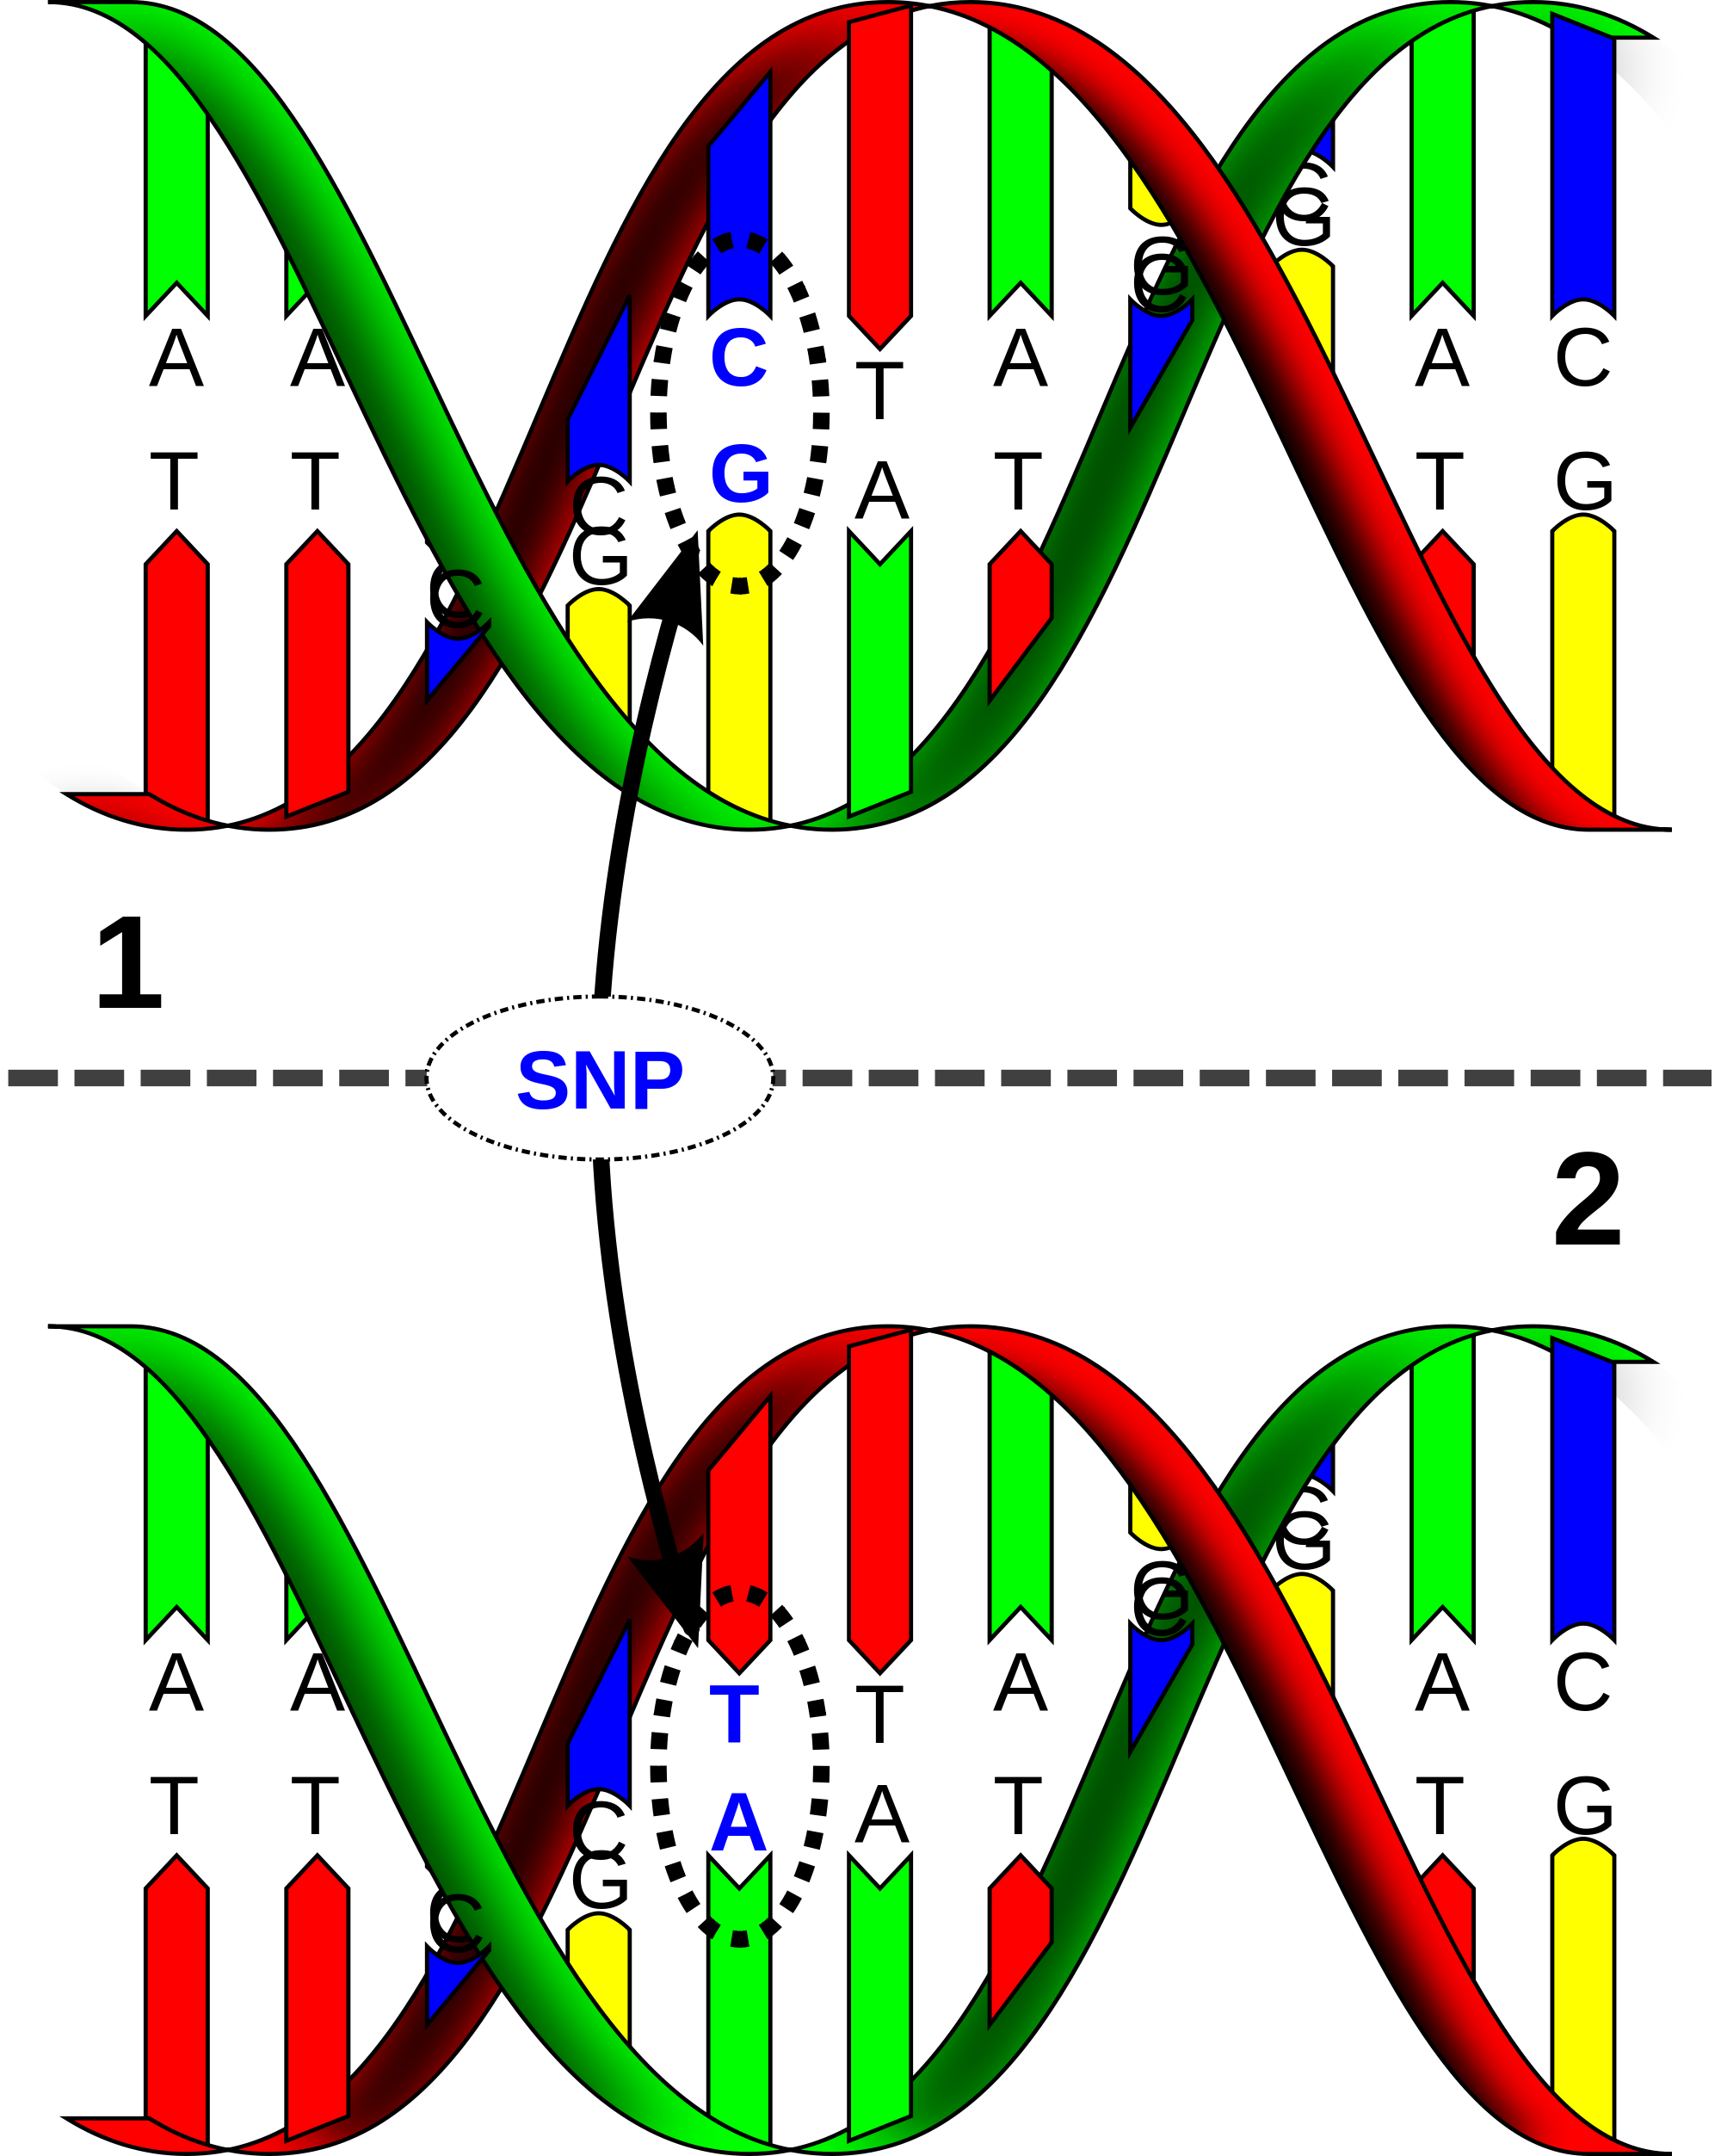
\includegraphics[width=0.8\textwidth]{{{figure/2000px-Dna-SNP.svg}}}
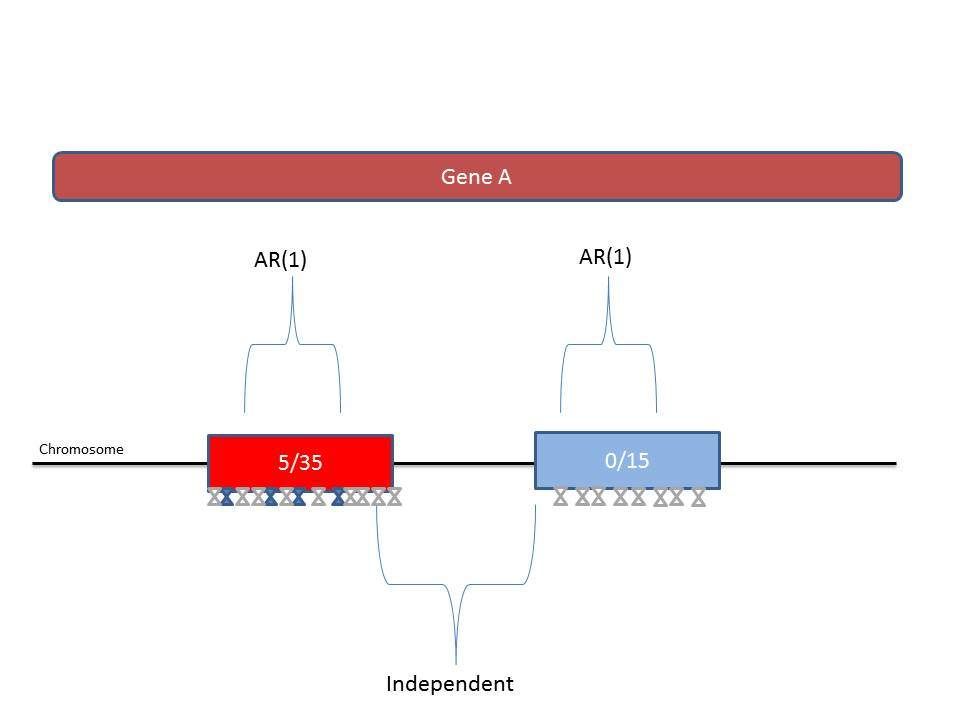
\includegraphics[height=0.6\textheight]{{{figure/genotype_simulation_demo}}}
\caption{ Demo graph of genotype simulation}
\end{figure}

%
%As a summary, we simulated genotypes following
%Wang and Elston.\cite{Wang2007}.\\
%\begin{enumerate}
%\item a latent vector $G_i = (G_{i1}, \ldots, G_{ip})'$ was first drawn from  a \textbf{multivariate Normal distribution} $N(0,R)$, where $R$ had a AR(1) correlation structure with its $(i,j)$th element in terms of purely correlation $r_{ij} =\textrm{Corr} (G_{if}, G_{ig}) = \rho ^ { |f - g| }$ between any two latent components, $G_{if}$ and $G_{ig}$ for $f \neq g$. In our simulations we set $\rho = 0.8$.;
%\item the latent vector $G_i$ was dichotomized to yield a haplotype with each latent element $G_{ij}$ dichotomized to 0 or 1 with probability $\textrm{Prob} (G_{ij} = 1) = $ MAF of $j$th SNP; the MAFs were randomly drawn from a uniform distribution: for causal SNPs the MAFs were set between 0.3 and 0.4; for null SNPs the MAFs were set between 0.1 and 0.5;
%\item we combined two independent haplotypes to form the genotype $X_i = (X_{i1}, \ldots, X_{ip})' $ for subject $i$. The haplotypes for different subject were generated independently.
%\end{enumerate}

%\scriptsize
%By this strategy we placed 35 SNPs in first block with AR(1) correlation structure to imitate the real LD structure among these SNPs; out of 35 SNPs we randomly set 5 SNPs to be causal (i.e. has a non-zero coefficient in later introduced regression model); to mimic the real data situation in SNP genotyping platforms, e.g. tag SNPs are usually in LD with causal SNPs but not the causal SNPs themselves, we excluded the 5 causal SNPs in the test (thus in first block, only null SNPs in LD with these 5 causal SNPs will enter the test). We further placed 15 null SNPs in the second block with AR(1) correlation structure as the same as we did in the first block. Note the first block and second block are independent though. All the SNPs from second block will participate in the test.

\framebreak
\textbf{Simulation of phenotype data}\\\

We setup the mixed effect model to achieve the AR(1) correlation structure as:\\
\begin{equation}
y_{im} = \mu_{i} + b_i + \underbrace{ \rho e_{i,m-1} + s_{i,m} }_{ e_{i,m} }  ,
\label{eq:y_im_split}
\end{equation}
with $m = 1,\ldots,k$ indexes the longitudinal measurements within subject $i$; $$\mu_{i} = Z_i \varphi + X_i \beta = H_i \theta$$ as in quantitative trait case; $b_i$ is the random intercept representing the subject-level random effect, and
$$
\rho e_{i,m-1} + s_{i,m} = e_{i,m},
$$ 
where $\rho$ is lag-one autocorrelation coefficient, so we can plugin our estimate from real data here by setting up $\rho = 0.7$. We assume the following distribution:\\
\begin{align*}
b_i & \sim N(0,\sigma_b^2)\\
e_{i,m} & \sim  N(0, \sigma_e^2)\\
s_{i,m} & \sim  N(0, (1 - \rho^2) \sigma_e^2 )
\end{align*}
Under this assumption, the variance-covariance matrix across longitudinal measurements becomes (assuming $k = 4$ for the number of longitudinal measurements ):
\begin{eqnarray}
\Sigma_{4\times 4} = Var 
\begin{pmatrix}
b_i + e_{i1}\\
b_i + \rho e_{i1} + s_{i2}\\
b_i + \rho e_{i2} + s_{i3}\\
b_i + \rho e_{i3} + s_{i4}
\end{pmatrix}
= \sigma_b^2
\begin{pmatrix}
1 & 1 & 1 & 1\\
1 & 1 & 1 & 1\\
1 & 1 & 1 & 1\\
1 & 1 & 1 & 1
\end{pmatrix}
+ \sigma_e^2 
\begin{pmatrix}
1 & \rho & \rho^2 & \rho^3 \\
\rho & 1 & \rho & \rho^2 \\
\rho^2 & \rho & 1 & \rho \\
\rho^3 & \rho^2 & \rho & 1
\end{pmatrix}
\label{eq:v-cov_split}
\end{eqnarray}

%\framebreak
%\textbf{Connect phenotype data with genotype data}\\
%Let we first introduce the below splitting of the phenotype variance:
%\begin{align}
%Var(y_{im} ) & = Var(X_{ij}) \beta_j^2 + \sigma_{oth} ^ 2  = 2f(1-f) \beta_j^2 + \sigma_{oth}^2
%\label{eq:variance_split_ge_oth}
%\end{align}
%%where the Hard-Weinberg equilibrium is assumed to hold. $f$ is the MAF of the SNP; $\sigma_{oth}^2$ is the residual variance after removing the effect of $j$th SNP. Obviously we can see $\sigma_b^2$ and $\sigma_e^2$ are contained in $\sigma_{oth}^2$ (see equation \eqref{eq:y_im_split}), and if other SNPs' effect are negligible, we expect $\sigma_b^2 + \sigma_e^2 \approx \sigma_{oth}^2$. 
%Now let we look at the relationship between genetic heritability (narrow-sense heritability) and equation \eqref{eq:variance_split_ge_oth}:
%\begin{align}
%h^2 = \frac{Var(A)}{Var(P)}
%\end{align}
%%this is the classical formula of narrow-sense heritability, with $Var(A)$ represents the variance due to the additive effects of the alleles, and $Var(P)$ represents the total variance in the phenotype. 
%In our situation for $j$th SNP, this can be extended to:
%\begin{align}
%h_j^2 = \frac{Var_j(A)}{Var(P)} = \frac{Var(X_{ij}) \beta_j^2 } {Var(y_{im} )} = \frac{Var(y_{im} ) - \sigma^2_{oth} } {Var(y_{im} )} \approx \frac{Var(y_{im} ) - \sigma_b^2 - \sigma_e^2 } {Var(y_{im} )}
%\label{eq:h_j_derive_to_var_y_im}
%\end{align}

\framebreak
\textbf{Summary of parameter setup in simulation studies}\\\

%After this point, by systematically solving the equations \eqref{eq:variance_split_ge_oth} and \eqref{eq:h_j_derive_to_var_y_im}, we can easily calculate the $\beta_j$ for $j$th SNP once we have determined the value of $h_j^2$, $\sigma_b^2$, $\sigma_e^2$ and $f$. Usually a $h_j^2$ for a single SNP $j$ will not be high for complex disease and we used $h_j^2 = 0.001$ in our simulation study to control $\beta_j$.
%We summarize the parameters used in simulation studies here:
\begin{itemize}
\item $h_j^2 = 0.001$
\item $\sigma_b = 7$
\item $\sigma_e = 27$
\item $n$ varies between $500$ and $3000$ 
\item $k = 4$
\item 1000 replicates of simulated dataset
\item $\alpha = 0.05$
\item $\rho_y = 0.7$
\item $\rho_x = 0.8$
\item $R = AR(1)$
\item $Rw = I$
\end{itemize}

% with other parameters set as: $\sigma_b^2 = 1$, $\sigma_e^2 = 1$ and $k = 4$ representing the number of longitudinal measurements for a single subject. Without special indication, we will use the simulated data set with 1000 replicates; significance level is set at 0.05. \\ 
\end{frame}

%%%%%%%%%%%%%%%%%%%%%%%%%%%%%%%%%%%
%%%%%%%%%%%%%%%%%%%%%%%%%%%%%%%%%%%
\subsubsection{Simulation Results}
\frame{
\frametitle{Table of Contents}
\small
\tableofcontents[currentsection,currentsubsection]
}
%5
\begin{frame}[allowframebreaks]
\frametitle{Simulation Results}
\framesubtitle{Journal Article 1}
\scriptsize
\begin{itemize}
\item \textbf{Simulation setting A}
%
\begin{itemize}
\item $B = 1000$ for simulation of $U$
\item sample size of 500, 1000, 2000 and 3000
\item 5/15 + 0/35 SNPs allocation
\item 0.05 $<$ MAF $<$ 0.4
\item $h_j^2 = 0$ 
\item $\alpha = 0.05$
\end{itemize}



%%%%%%
\begin{center}
\tiny
\begin{table}[H]
\begin{tabular}{lcccccccccccc}
\hline 
n & pSSU & pSSUw & pScore & pSum & pUminP  & LaSPU & LaSPUw & LaSPU.sco & LaSPU.omni \\
\hline 
 500 & 0.047 & 0.048 & 0.047 & 0.052 & 0.048   & 0.060 & 0.058 & 0.058  & 0.058 \\
1000 & 0.047 & 0.046 & 0.044 & 0.058 & 0.048   & 0.057 & 0.057 & 0.057  & 0.057 \\
2000 & 0.049 & 0.047 & 0.051 & 0.048 & 0.048   & 0.061 & 0.058 & 0.058  & 0.058 \\
3000 & 0.051 & 0.052 & 0.052 & 0.052 & 0.050   & 0.063 & 0.060 & 0.059  & 0.059 \\
\hline 
\end{tabular}
% \vspace{-1em}%%%%%%%%% reduce the space between table and text
% \captionof{table}{Type I error using working independence Rw}
\caption{ Empirical Type I Error Table in the simulation setting A}
\label{table:type_I_error_CV_varySampleSize}
\end{table}
\end{center}
%%%%%%%%%%%%%%%%%%%

\framebreak
\begin{minipage}[t]{0.3\linewidth}
\item \textbf{Simulation setting B}
\begin{itemize}
\item $h_j^2 = 0.001$
\end{itemize}
\end{minipage}%
\hfill%
% 
\begin{minipage}[t]{0.7\linewidth}
\begin{figure}[H]
\centering
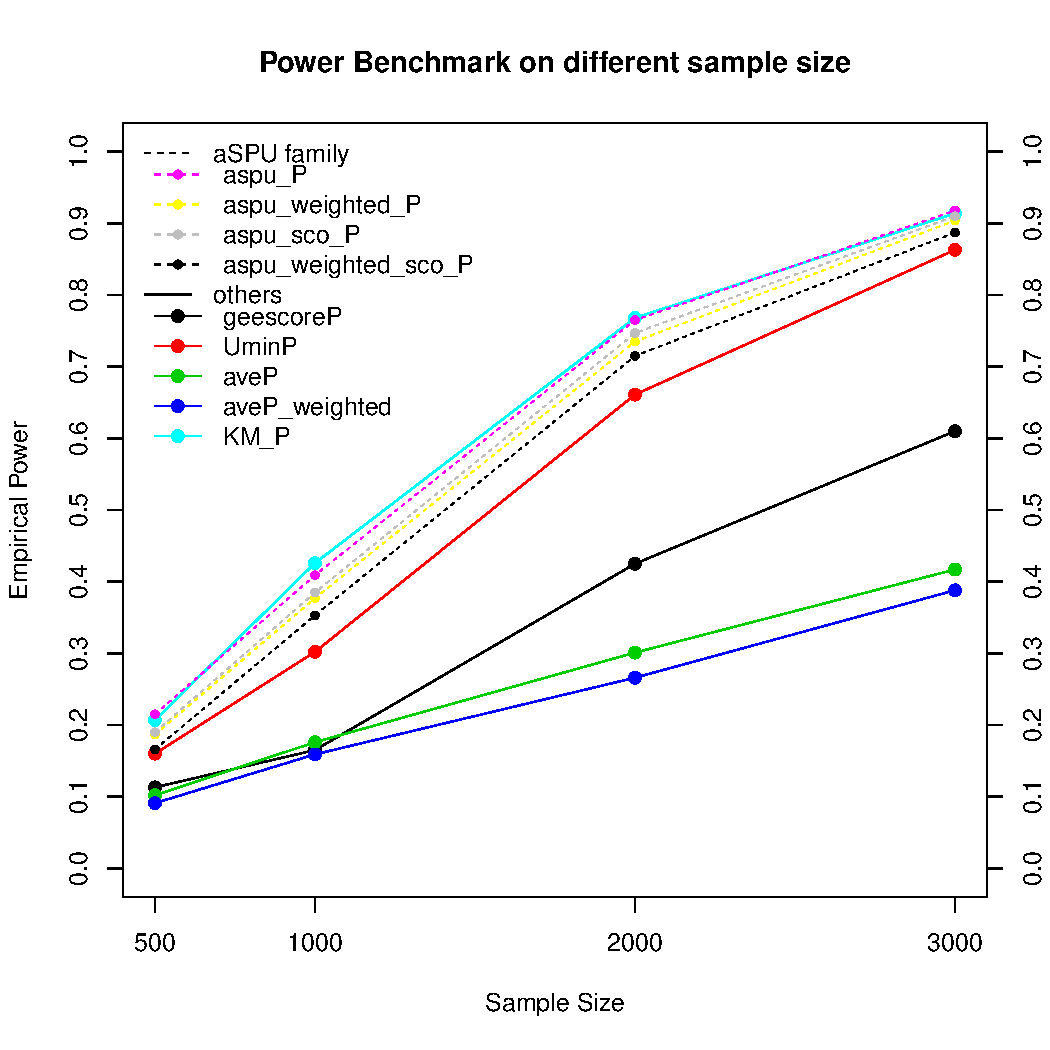
\includegraphics[height=0.7\textheight]{{{figure/PowerCurve_independenceWkCor_on_AR1data_h0.001}}}
\vspace{-15pt}
\caption{Empirical power benchmark under different $n$ in the simulation setting B.}
\label{fig: PowerCurve_independenceWkCor_on_AR1data_h0.001}
\end{figure}
\end{minipage}


\newpage
\item \textbf{Simulation setting C}
\begin{columns}[T]
\begin{column}{0.3\textwidth}
\begin{itemize}
\item 3(+) and 2(-) in 5 causal SNPs
\end{itemize}
\end{column}%
\hfill%
%%%%%%%%%%%%%%%%%%% 
\begin{column}{0.7\textwidth}
\begin{figure}[H]
\centering
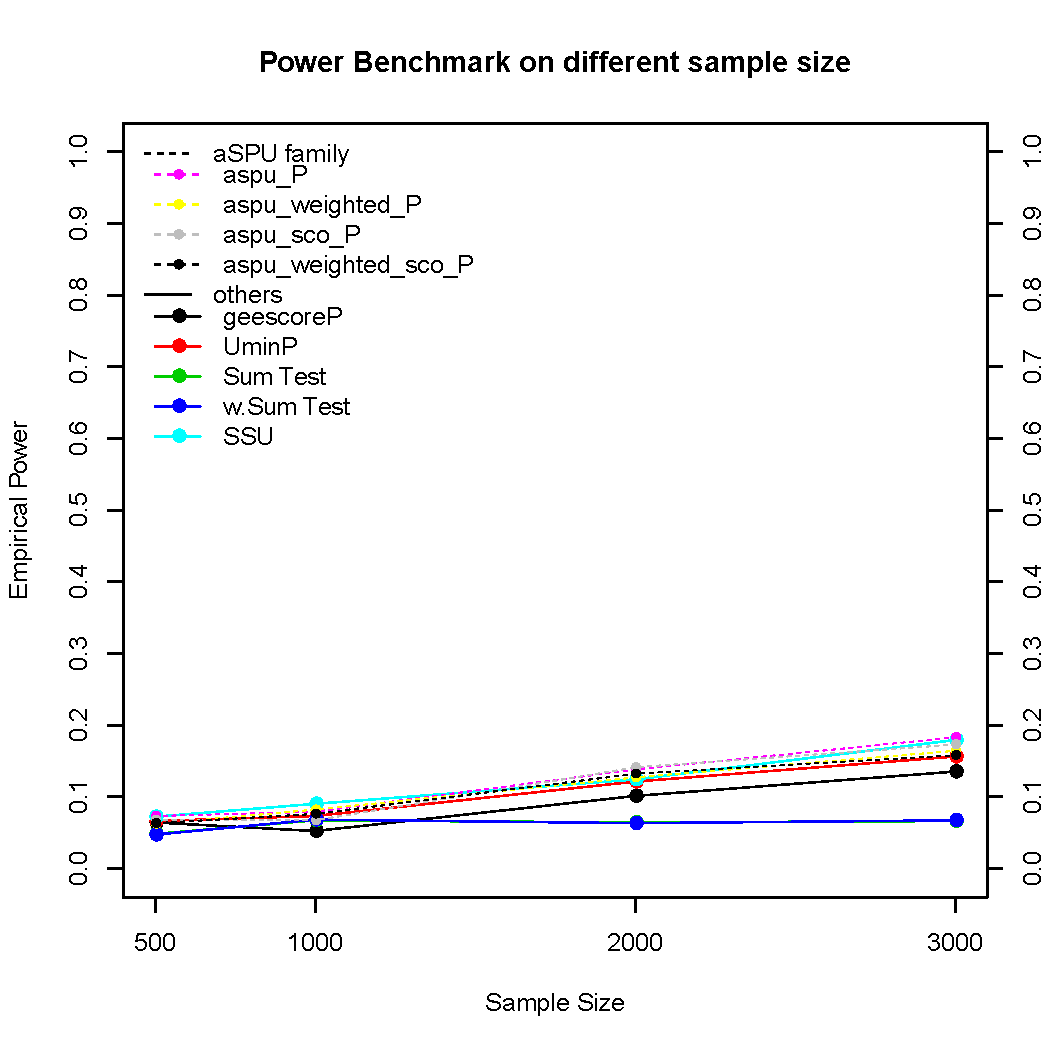
\includegraphics[height=0.7\textheight]{{{figure/PowerCurve_independenceWkCor_on_AR1data_h0.001_heterogeneousSNPeffects}}}
\vspace{-15pt}
\caption{Empirical power benchmark under a heterogeneous SNP effects in the simulation setting C.}
\label{fig: PowerCurve_independenceWkCor_on_AR1data_h0.001_heterogeneousSNPeffects}
\end{figure}
\end{column}%
\end{columns}

\framebreak
\vspace{-10pt}
\scriptsize
\item  \textbf{Simulation setting D: Testing with a growing number of null SNPs (in the second block)}\\
%In previous two tests scenarios, we confirmed the ability of aSPU family members and concluded the SPU(2) is most powerful and contribute to the good performance of aSPU family. Now we are curious how higher $\gamma$ will bring aSPU family to the edge. We gradually increased the number of null SNPs number from 50 to 75, 100, 200, then finally a seemingly extreme number 400. We used $n = 3000$ as the sample size. We kept all other settings the same with previous scenarios. The empirical power benchmark result is shown below:
%%%%%%%%%%%%%%%%%%%%%%
\begin{figure}[H]
\centering
\vspace{-10pt}
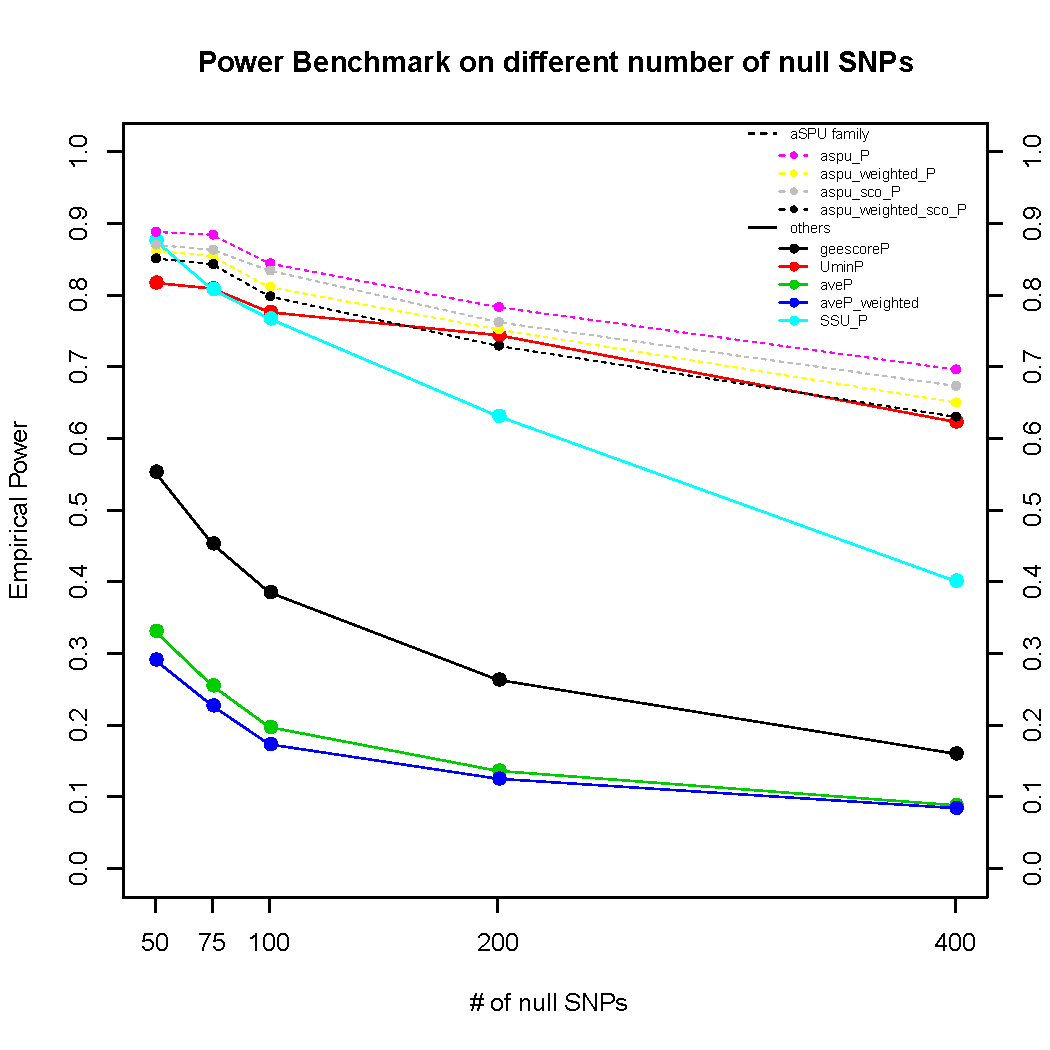
\includegraphics[height=0.7\textheight]{{{figure/PowerCurve_independenceWkCor_on_AR1data_h0.001_withNSNPnull}}}
\vspace{-15pt}
\caption{\tiny Empirical power benchmark under an increased number of null SNPs in the simulation setting D.}
\label{fig: PowerCurve_independenceWkCor_on_AR1data_h0.001_withNSNPnull}
\end{figure}

\newpage
\item \textbf{Simulation setting E: assessing power gain from longitudinal measurements}
\begin{figure}[H]
\centering
\vspace{-10pt}
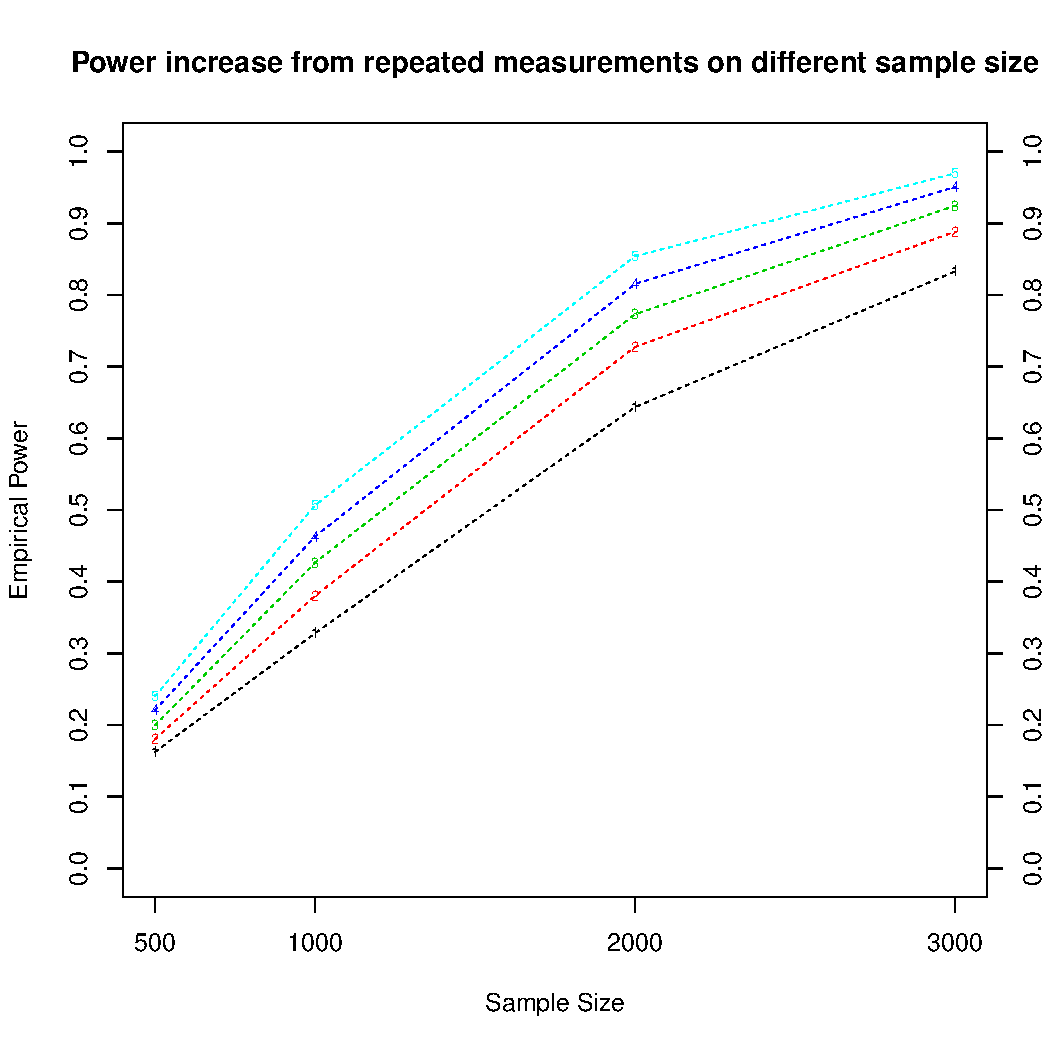
\includegraphics[height=0.7\textheight]{{{figure/PowerIncreaseCurve_independenceWkCor_on_AR1data_h0.001_CVs_simulatedInCorrelatedResidual}}}
\vspace{-15pt}
\caption{\footnotesize Power increases from repeated measurements in the simulation setting E.}
\label{fig: PowerLongiIncreaseCurve_independenceWkCor_on_AR1data_h0.001}
\end{figure}
\end{itemize}
\end{frame}

%-------------------------------------------------------------------------------------------------%
\begin{frame}[allowframebreaks]
\footnotesize
\frametitle{Simulation Results for Rare Variants}
\framesubtitle{Journal Article 1}
\begin{itemize}
\item \textbf{Simulation setting A'}
\begin{itemize}
\item 5/15 with 5 included in the test
\item 0.001 $<$ MAF $<$ 0.01
\end{itemize}
\begin{table}[ht]
\centering
\tiny
\begin{tabular}{cccccccccccccccccccc}
  \hline
n    & pSSU & pSSUw & pScore & pSum & pUminP  & LaSPU & LaSPUw & LaSPU.sco &  LaSPU.omni\\
  \hline
500  & 0.053 & 0.054 & 0.052 & 0.049 & 0.047  & 0.054 & 0.053 & 0.060   & 0.058 \\
1000 & 0.055 & 0.040 & 0.042 & 0.048 & 0.054  & 0.047 & 0.045 & 0.052   & 0.051 \\
2000 & 0.054 & 0.050 & 0.048 & 0.049 & 0.046  & 0.063 & 0.057 & 0.058   & 0.057 \\
3000 & 0.045 & 0.044 & 0.039 & 0.060 & 0.053  & 0.049 & 0.053 & 0.049   & 0.053 \\
\hline
\end{tabular}
\caption{Empirical Type I Error Table in the simulation setting A'.  
\label{table:Empirical type I error using permutation-based method in RV analysis}}
\end{table}

\newpage
\item  \textbf{Simulation setting B'}
\begin{figure}[H]
\centering
\vspace{-10pt}
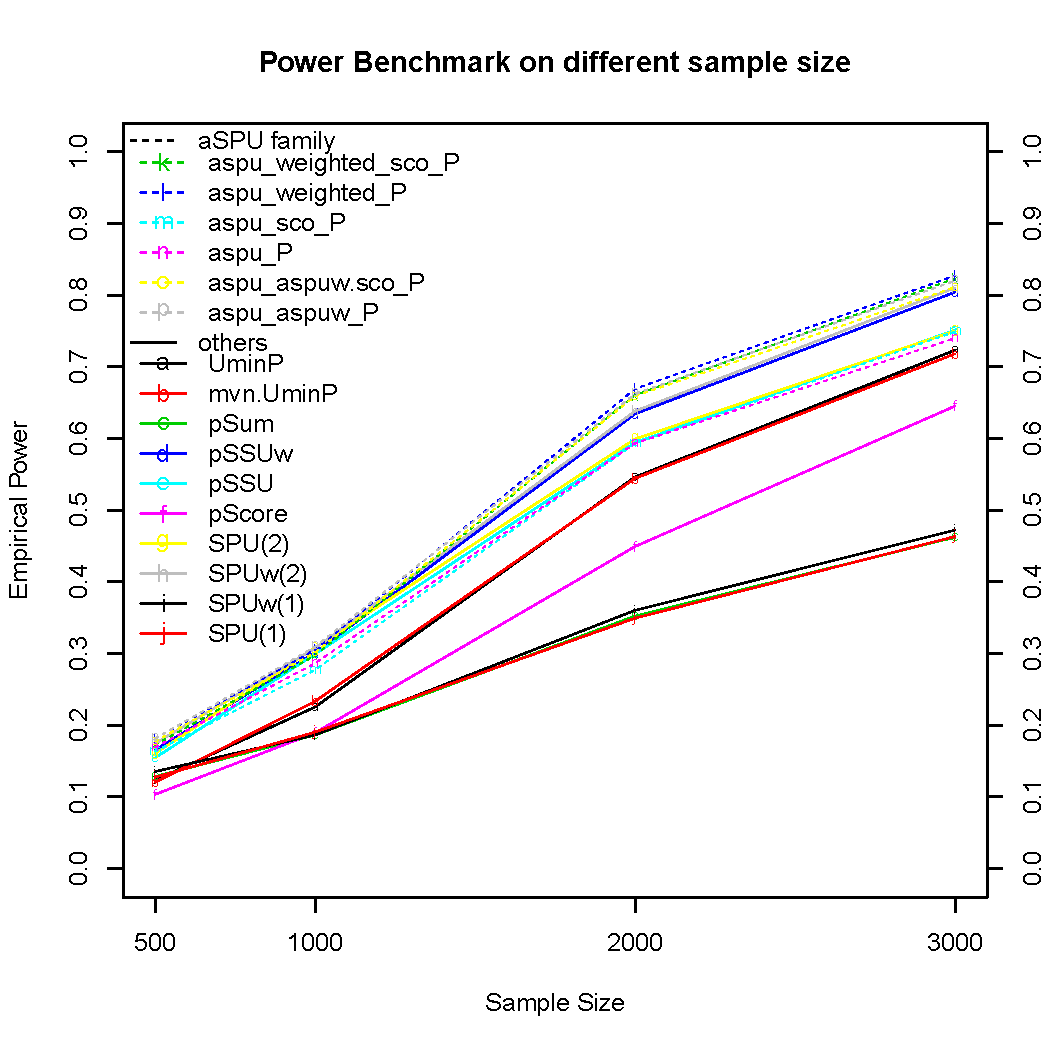
\includegraphics[height=0.7\textheight]{{{figure/PowerCurve_independenceWkCor_on_AR1data_h0.001_RVpermutedU_moreTests}}}
\vspace{-15pt}
\caption{\footnotesize Empirical power benchmark under different $n$ in the simulation setting B'.}
\label{fig: PowerLongiIncreaseCurve_independenceWkCor_on_AR1data_h0.001}
\end{figure}
\end{itemize}
\end{frame}

%-------------------------------------------------------------------------------------------------%
%%%%%%%%%%%%%%%%%%%%%%%%%%%%%%%%%%%
%%%%%%%%%%%%%%%%%%%%%%%%%%%%%%%%%%%
\subsubsection{Application to the ARIC Study}
\frame{
\frametitle{Table of Contents}
\small
\tableofcontents[currentsection,currentsubsection]
}
\begin{frame}[allowframebreaks]
\footnotesize
\frametitle{Application to the ARIC study}
\framesubtitle{Journal Article 1}
%------------------1---------------------%
\textbf{Methods in data application}\\\
\begin{itemize}
\item RV defined by MAF $<$ 0.05
\item Inclusion of only nonsynonymous and splice site variants
\item QC procedures as in \cite{Peloso2014}
\item Additive genetic model
\item Covariates include age, age$^2$, gender, BMI, time of measurement and top two PCs
\item Gene boundary defined in \cite{Peloso2014}
\item Significant: 0.05/25,000 = 2e-06; marginal significant: 1e-03
\end{itemize}

\framebreak
%------------------2---------------------%
\textbf{\footnotesize Results in data application: compare longitudinal method with baseline method}
\vspace{-10pt}
\begin{figure}[b]
\centering
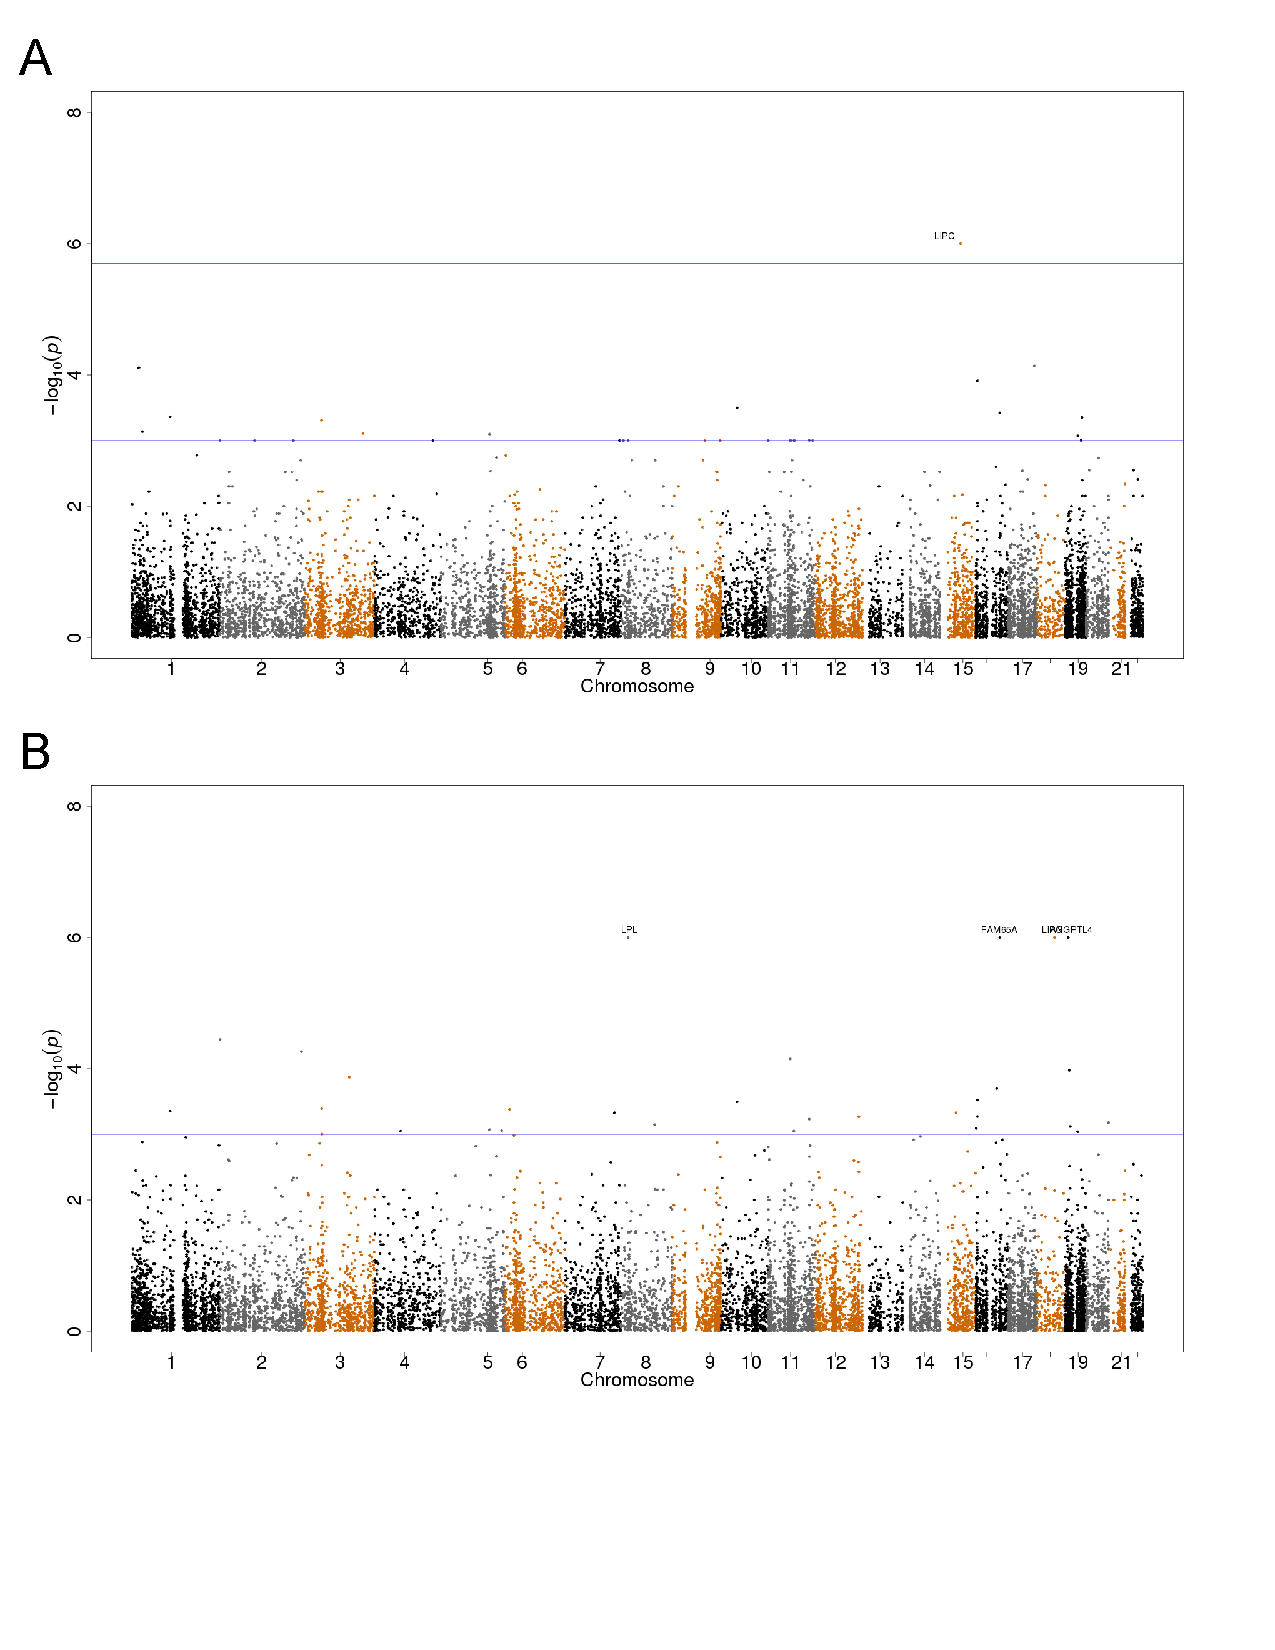
\includegraphics[height=0.76\textheight]{{{figure/compare_longi_LaSPU_exome_ARIC}}}
\vspace{-1cm}
\caption{\tiny Manhattan Plot Comparison between baseline study and longitudinal study by LaSPU test on the association between HDL-C and Rare Variants in the ARIC study. A. baseline study; B. longitudinal study using total four measurements.  }
\label{fig: compare_longi_LaSPU_exome_ARIC}
\end{figure}



\framebreak
%---------------------------------------%
\textbf{\footnotesize Results in data application: compare longitudinal method with baseline method}
\scriptsize
\ctable[
caption = {Top Gene-Based Association Results Based on Level of statistical Significance},
label = tab:table_gene_base,
pos = ht,
%width = 120mm,
center
%mincapwidth = \textwidth,
]{lcrrrrr}{
  \tnote[a]{\tiny number of variants contributing to the test}
  \tnote[b]{\tiny cumulative minor allele count of the variants contributing to
the test }
  \tnote[c]{\tiny cumulative minor allele frequency of the variants contributing to
the test}
  \tnote[d]{\tiny aSPU test using baseline only measurement of HDL-C}
  \tnote[*]{\tiny novelly identified gene(s)}
}{
														    \toprule[1pt]
  Gene & Chr & p Value & No.Variants\tmark[a] & CMAC\tmark[b] & CMAF\tmark[c] & p Value of Baseline\tmark[d] \ML[1pt]
  \textit{LPL} & 8 & 1.00E-06 & 10 & 879 & 0.00807 & 9.99E-04 \\
  \textit{FAM65A\tmark[*]} & 16 & 1.00E-06 & 11 & 751 & 0.00627 & 3.79E-04 \\
  \textit{LIPG} & 18 & 1.00E-06 & 11 & 369 & 0.00308 & 3.13E-02\\
  \textit{ANGPTL4} & 19 & 1.00E-06 & 9 & 579 & 0.00591 & 2.89E-01 \ML
  \textit{ANGPTL8} & 19 & 1.06E-04 & 5 & 64 & 0.00118 & 2.07E-01\\
  \textit{APOC3} & 11 & 5.87E-04 & 3 & 21 & 0.00064 & 9.99E-04\ML
  \textit{PAFAH1B2} & 11 & 2.19E-03 & 3 & 287 & 0.00879 & 1.50E-02\LL[1pt]
}


\framebreak
%---------------------------------------%
\textbf{\footnotesize Results in data application: compare LaSPU with LSSU method}
\begin{figure}[H]
\centering
\vspace{-10pt}
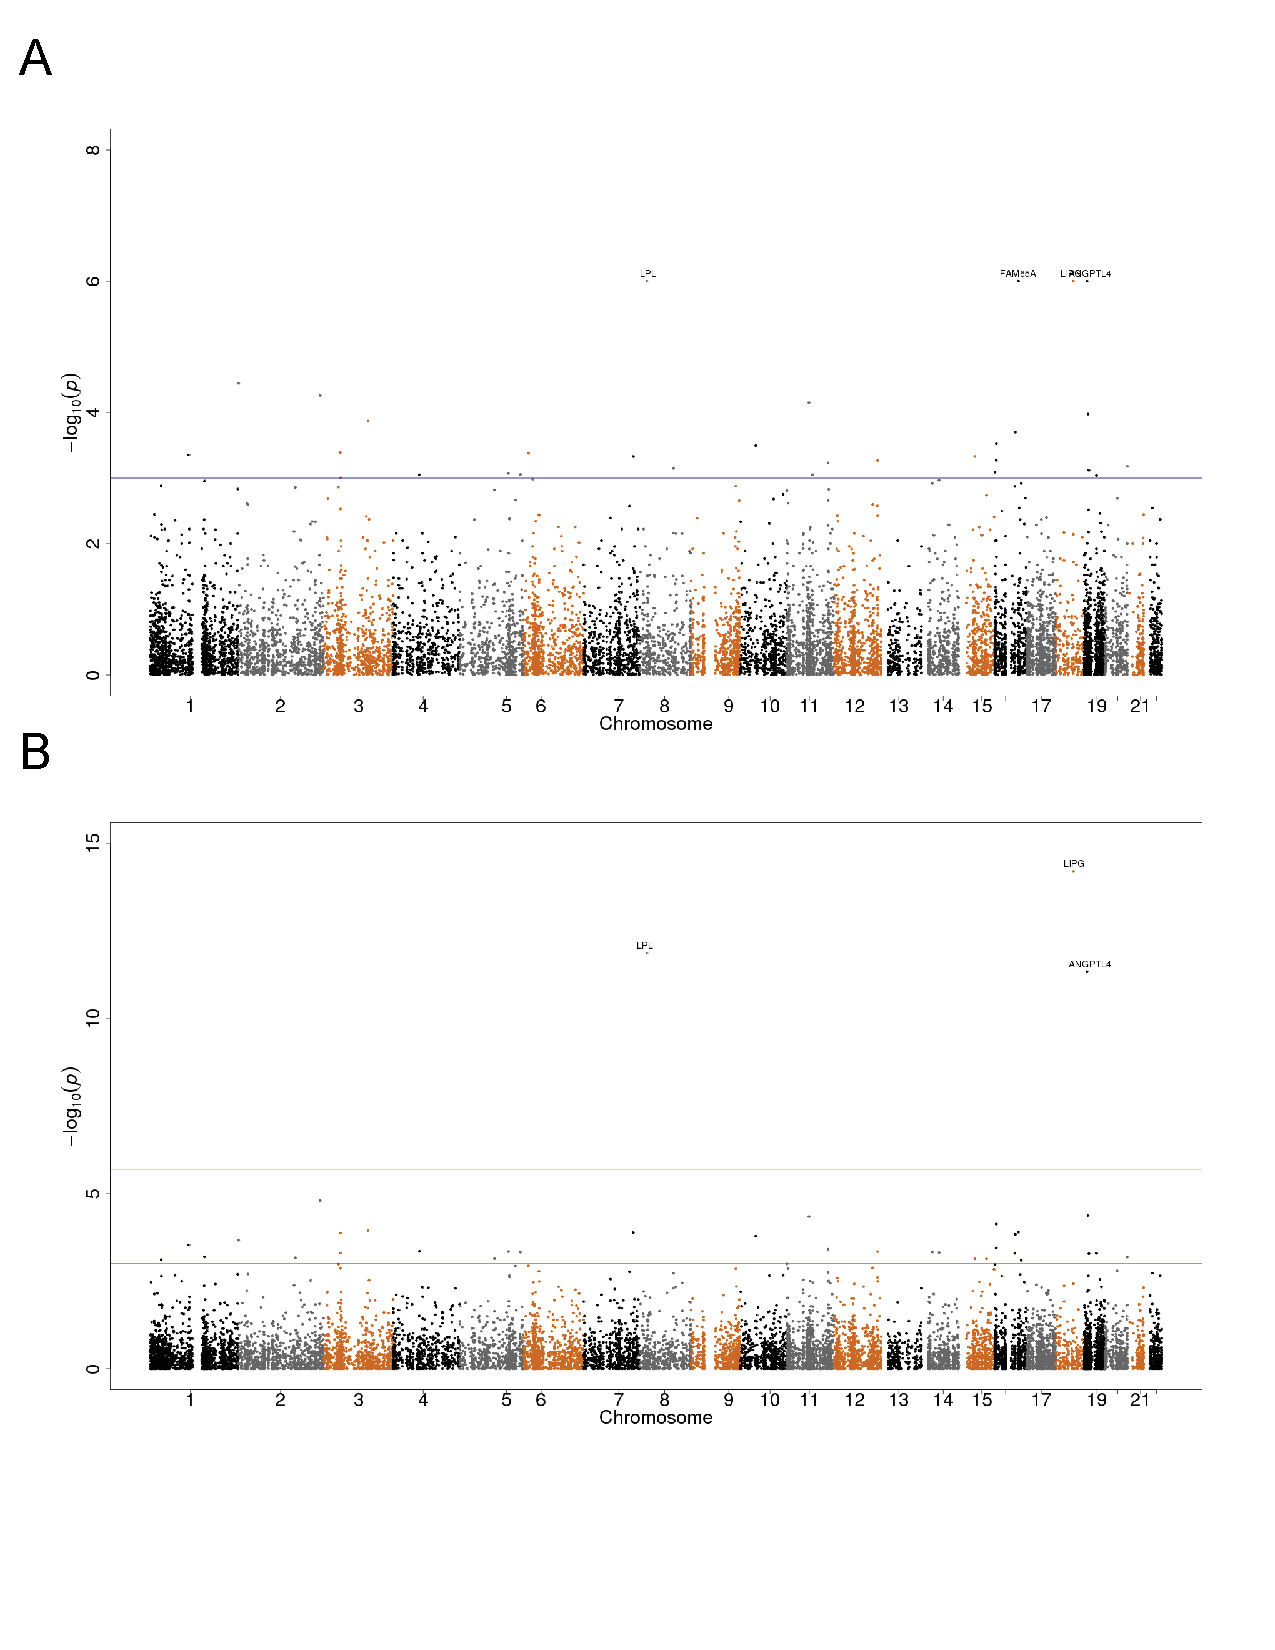
\includegraphics[height=0.76\textheight]{{{figure/compare_LaSPU_LSSU_exome_ARIC}}}
\vspace{-1cm}
\caption{\tiny Manhattan Plot Comparison between LaSPU test and LSSU test on the association between HDL-C and Rare Variants in the ARIC study. A. result by LaSPU; B. result by LSSU .  }
\label{fig: compare_LaSPU_LSSU_exome_ARIC}
\end{figure}


\framebreak
%---------------------------------------%
\textbf{\footnotesize Gene effect visualization of previously reported genes}
\begin{figure}[H]
\centering
\vspace{-10pt}
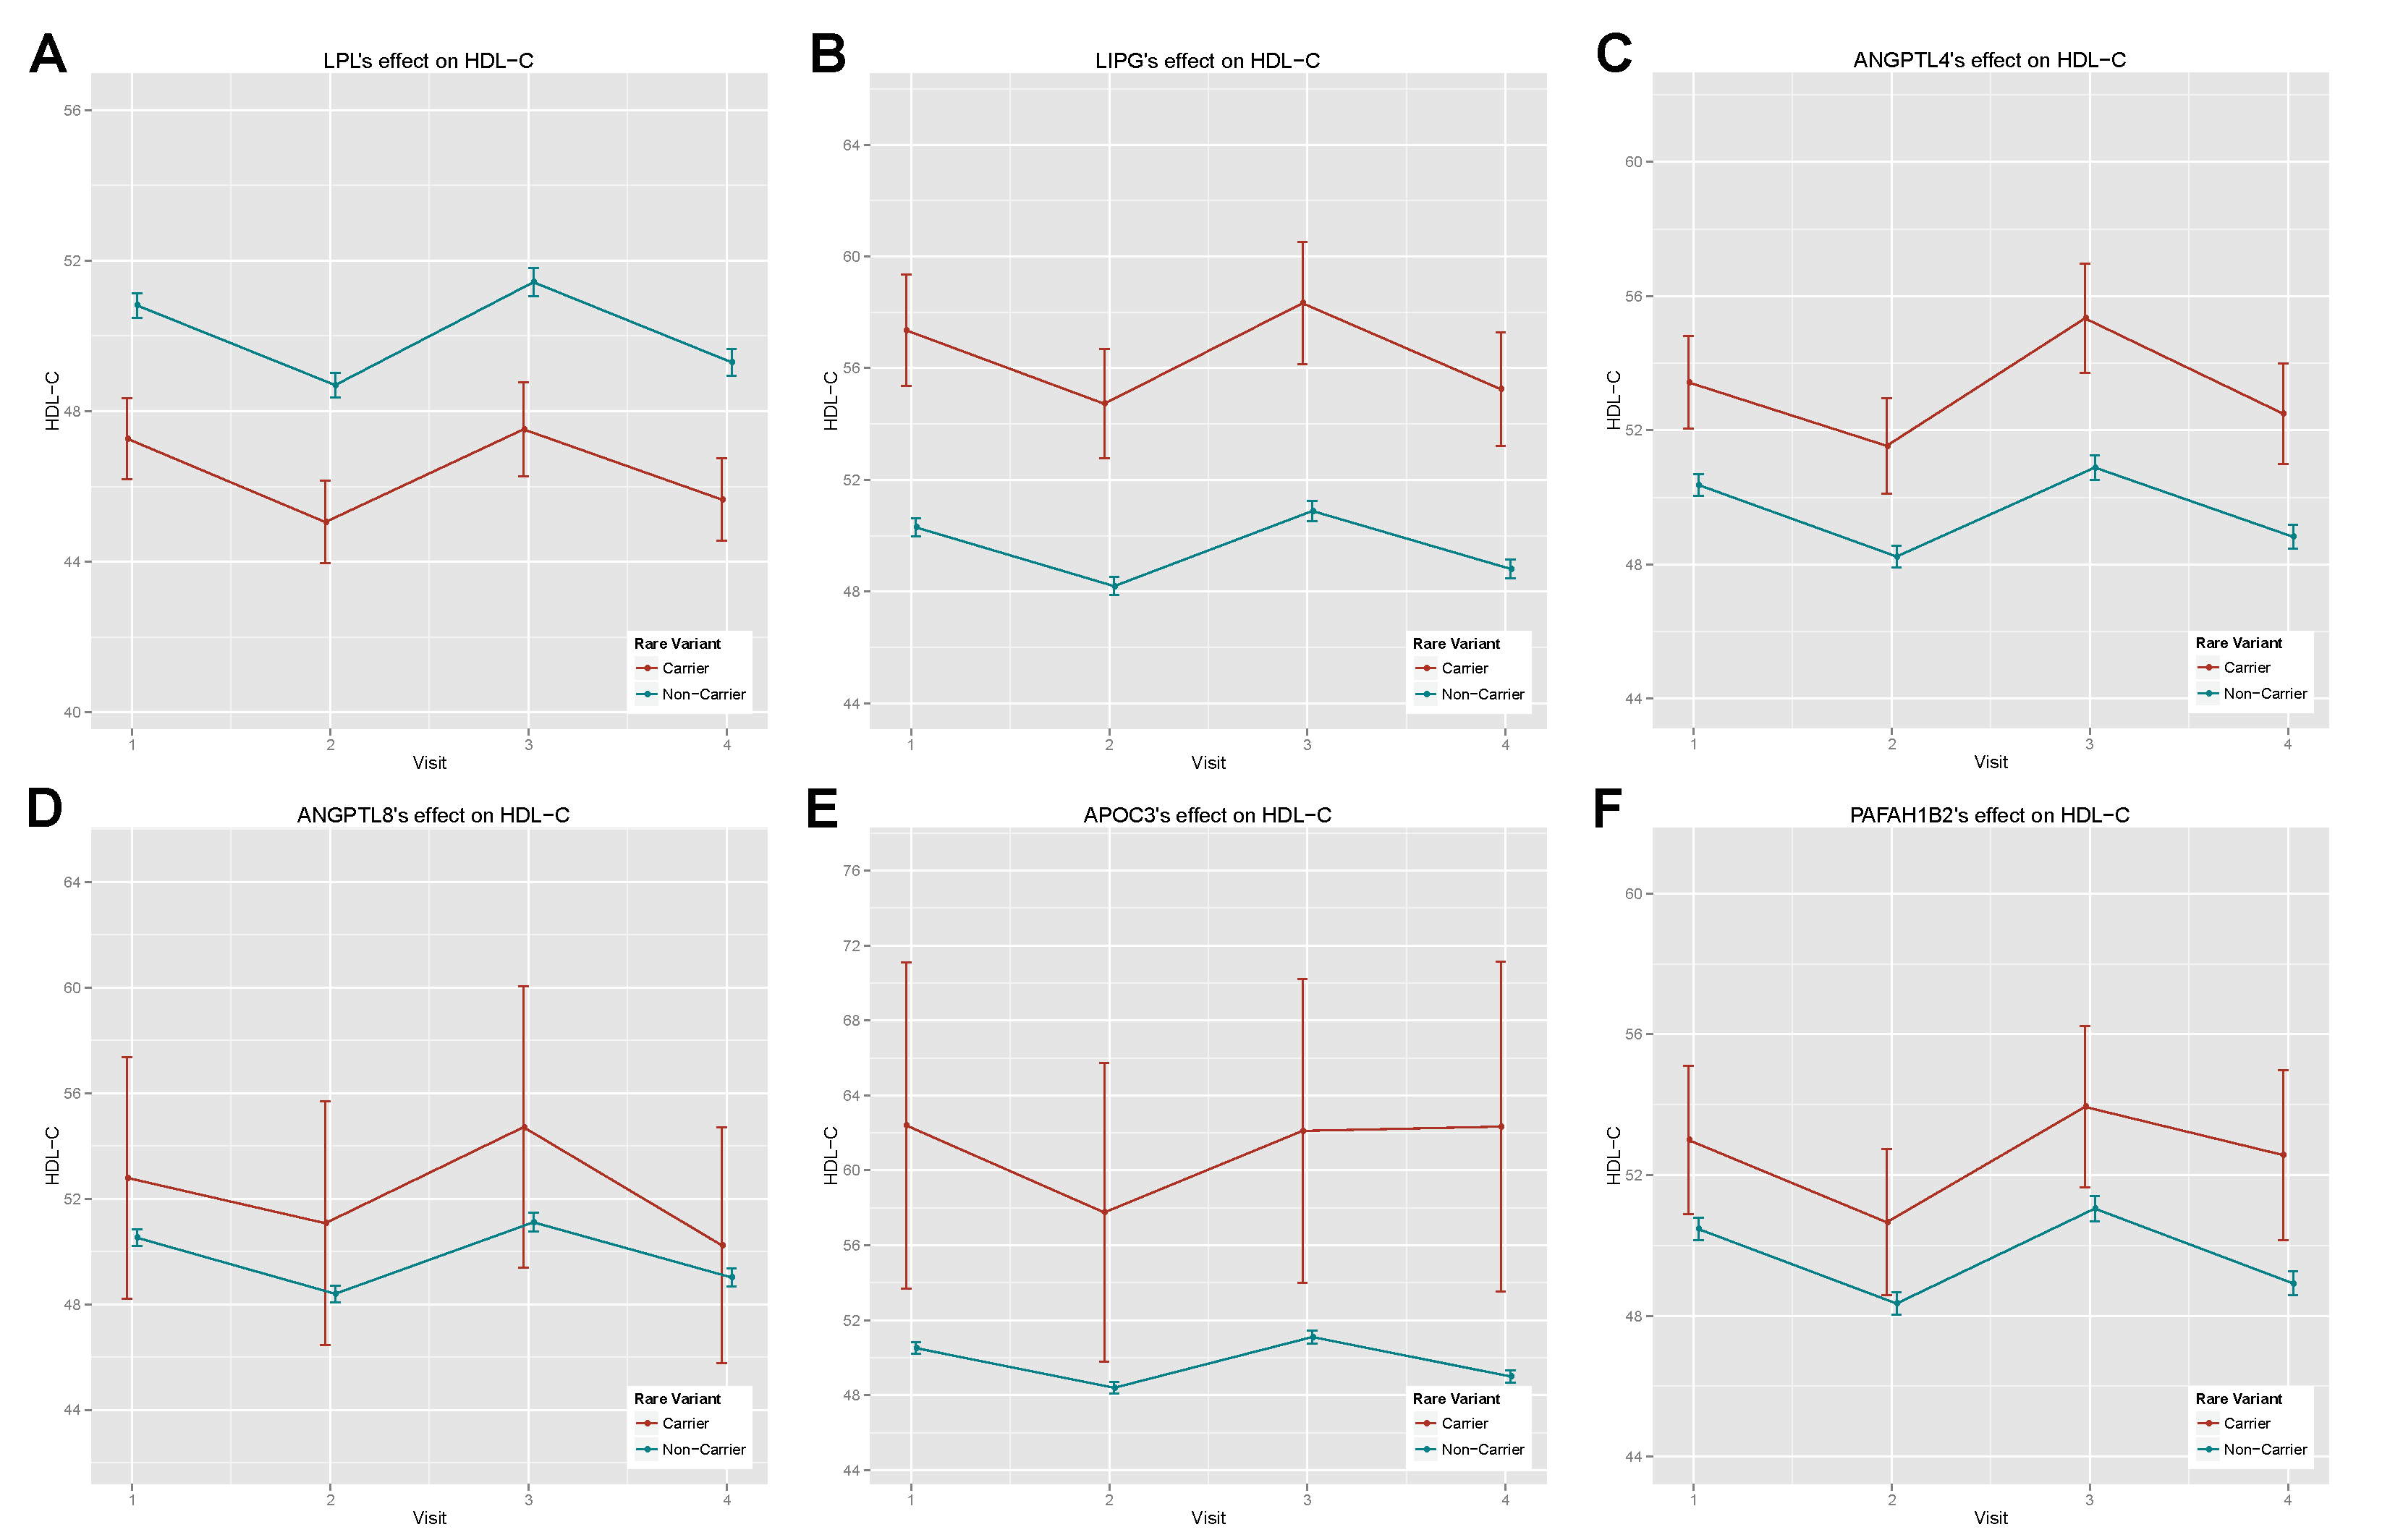
\includegraphics[height=0.76\textheight]{{{figure/known_signals_with_HDL_C}}}
\vspace{-1cm}
%\caption{\tiny }
\label{fig: known_signals_with_HDL_C}
\end{figure}

\framebreak
%---------------------------------------%
\textbf{\footnotesize Gene effect visualization of previously unreported genes}
\begin{figure}[H]
\centering
\vspace{-10pt}
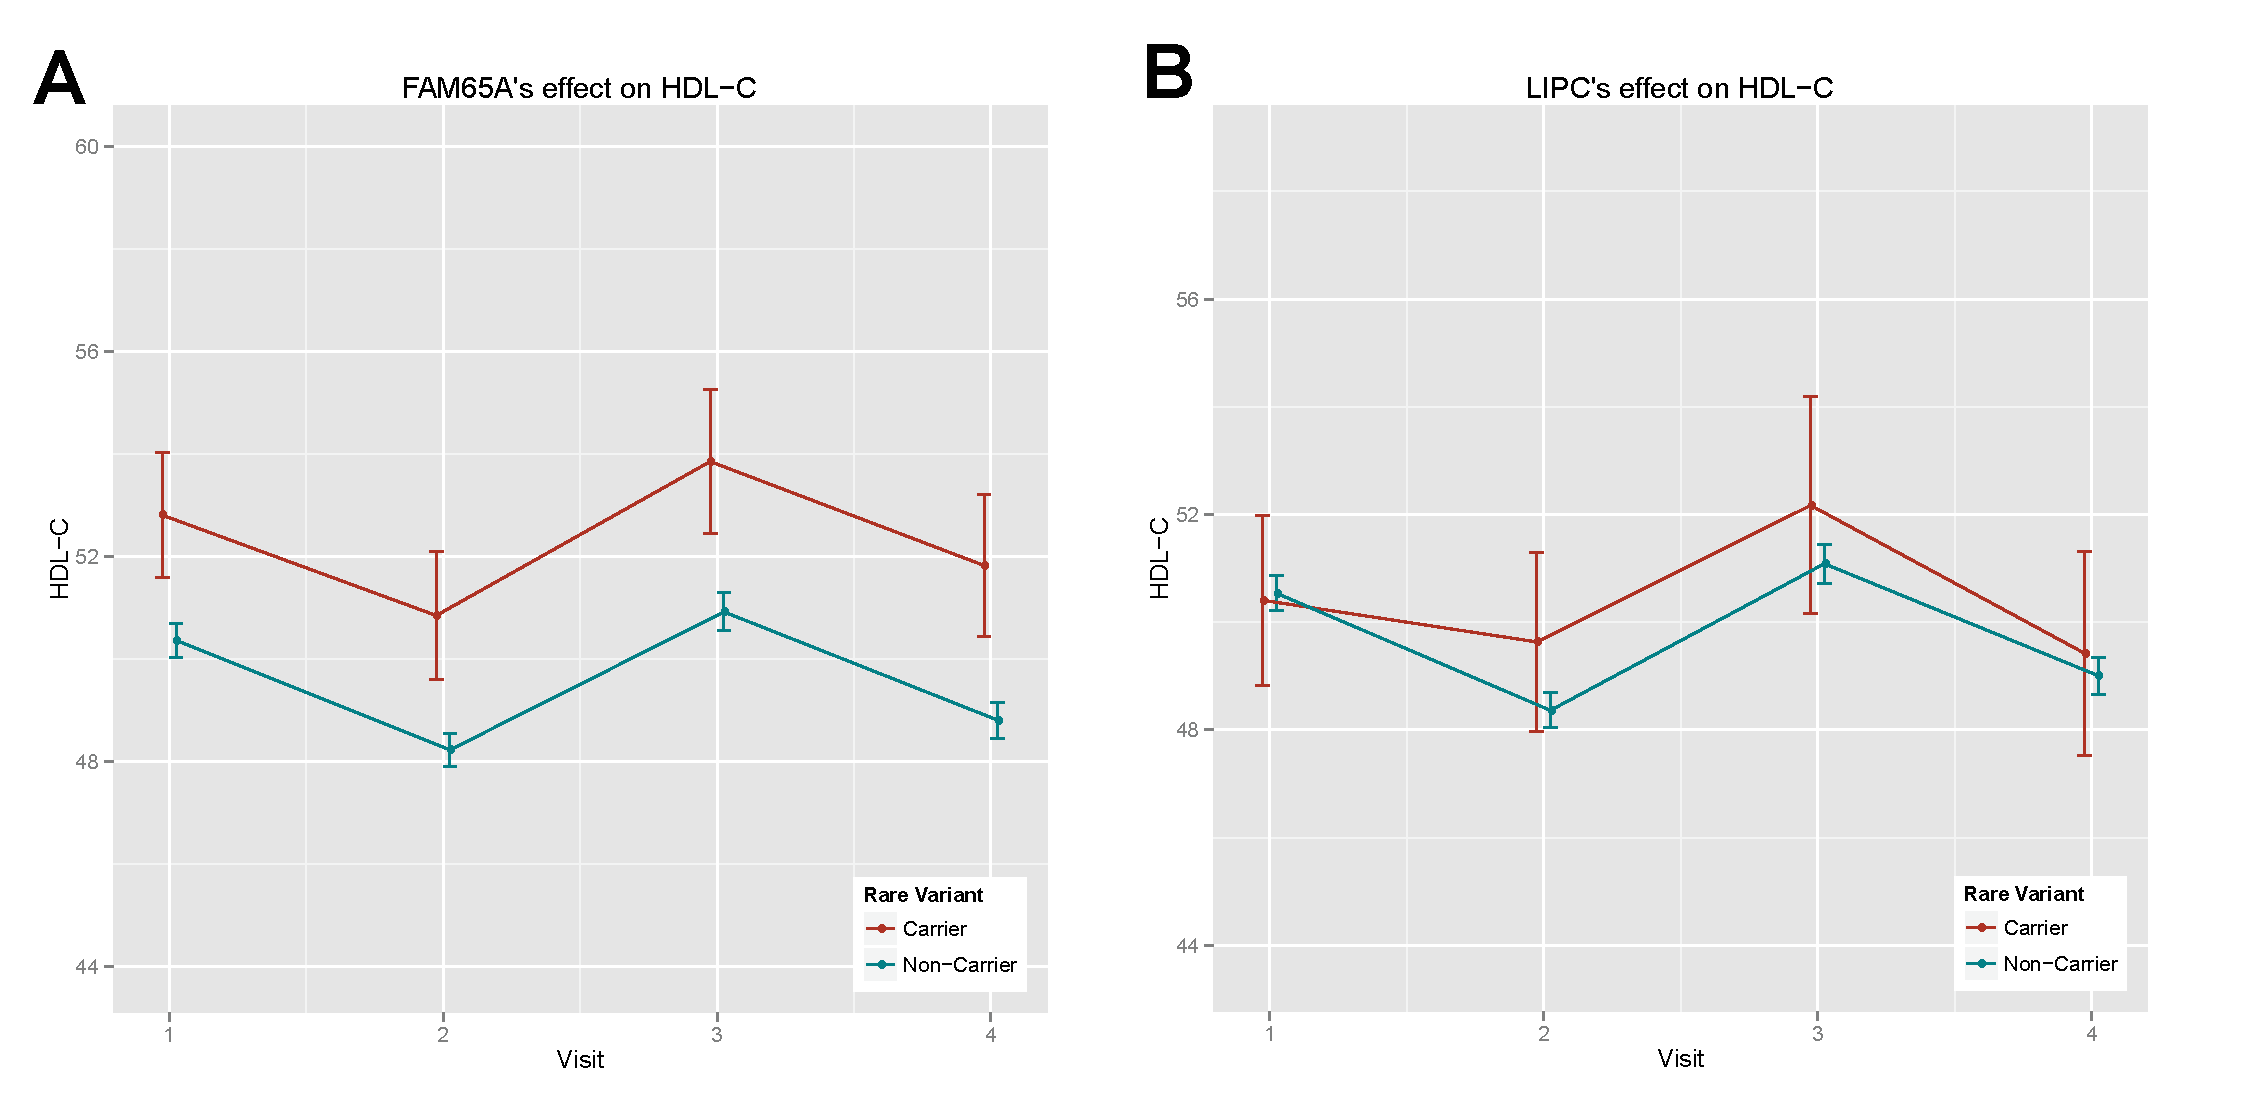
\includegraphics[width=0.8\linewidth]{{{figure/unreported_signals_with_HDL_C}}}
\vspace{-1cm}
%\caption{\tiny }
\label{fig: unreported_signals_with_HDL_C}
\end{figure}
\end{frame}


%-------------------------------------------------------------------------------------------------%
%%%%%%%%%%%%%%%%%%%%%%%%%%%%%%%%%%%
%%%%%%%%%%%%%%%%%%%%%%%%%%%%%%%%%%%
\subsubsection{Discussion}
\frame{
\frametitle{Table of Contents}
\small
\tableofcontents[currentsection,currentsubsection]
}
\begin{frame}[allowframebreaks]
\footnotesize
\frametitle{Discussion}
\framesubtitle{Journal Article 1}
%------------------1---------------------%
\begin{itemize}
\item LaSPU could efficiently use the longitudinal information to increase testing power
\item LaSPU could adaptively select the best test and achieve a greater power
\item LaSPU proved its ability in real data analysis by identifying the same reported genes associated with HDL-C using the ARIC data set only
\item LaSPU identified one novel gene associated with HDL-C: \textit{FAM65B}, which warrants further validation
\end{itemize}
\end{frame}






%%%%%%%%%%%%%%%%%%%%%%%%%%%%%%%%%%%%%%%%%%%%%%%%%%%
%%%%%%%%%%%%%%%%%%%%%%%%%%%%%%%%%%%%%%%%%%%%
%%%%%%%%%%%%%%%%%%%%%%%%%%%%%%%%%%%%%%%%%%%%%%%%%%%
\subsection{Journal Article 2: Pathway-based data-adaptive association tests ...}
%%%%%%%%%%%%%%%%%%%%%%%%%%%%%%%%%%%%%%%%%%%%%%%%%%%
%%%%%%%%%%%%%%%%%%%%%%%%%%%%%%%%%%%%%%%%%%%%
%%%%%%%%%%%%%%%%%%%%%%%%%%%%%%%%%%%%%%%%%%%%%%%%%%%
\frame{
\frametitle{Table of Contents}
\small
\tableofcontents[currentsection,currentsubsection]
}

%%%%%%%%%%%%%%%%%%%%%%%
%1
\frame{
\frametitle{Journal Article 2}
%\framesubtitle{Aim 1a}
\small
\textbf{Title of Journal Article}\\
Pathway-based data-adaptive association tests for longitudinal phenotypes.\\\

\textbf{Name of Journal Proposed for Article Submission}\\
American Journal of Human Genetics
}

\subsubsection{Methods}
\frame{
\frametitle{Table of Contents}
\small
\tableofcontents[currentsection,currentsubsection]
}
%2
\frame[allowframebreaks]{
\frametitle{Methods}
\framesubtitle{Journal Article 2}
\textbf{\footnotesize Pathway idea illustration}
\begin{figure}[H]
\centering
\vspace{-10pt}
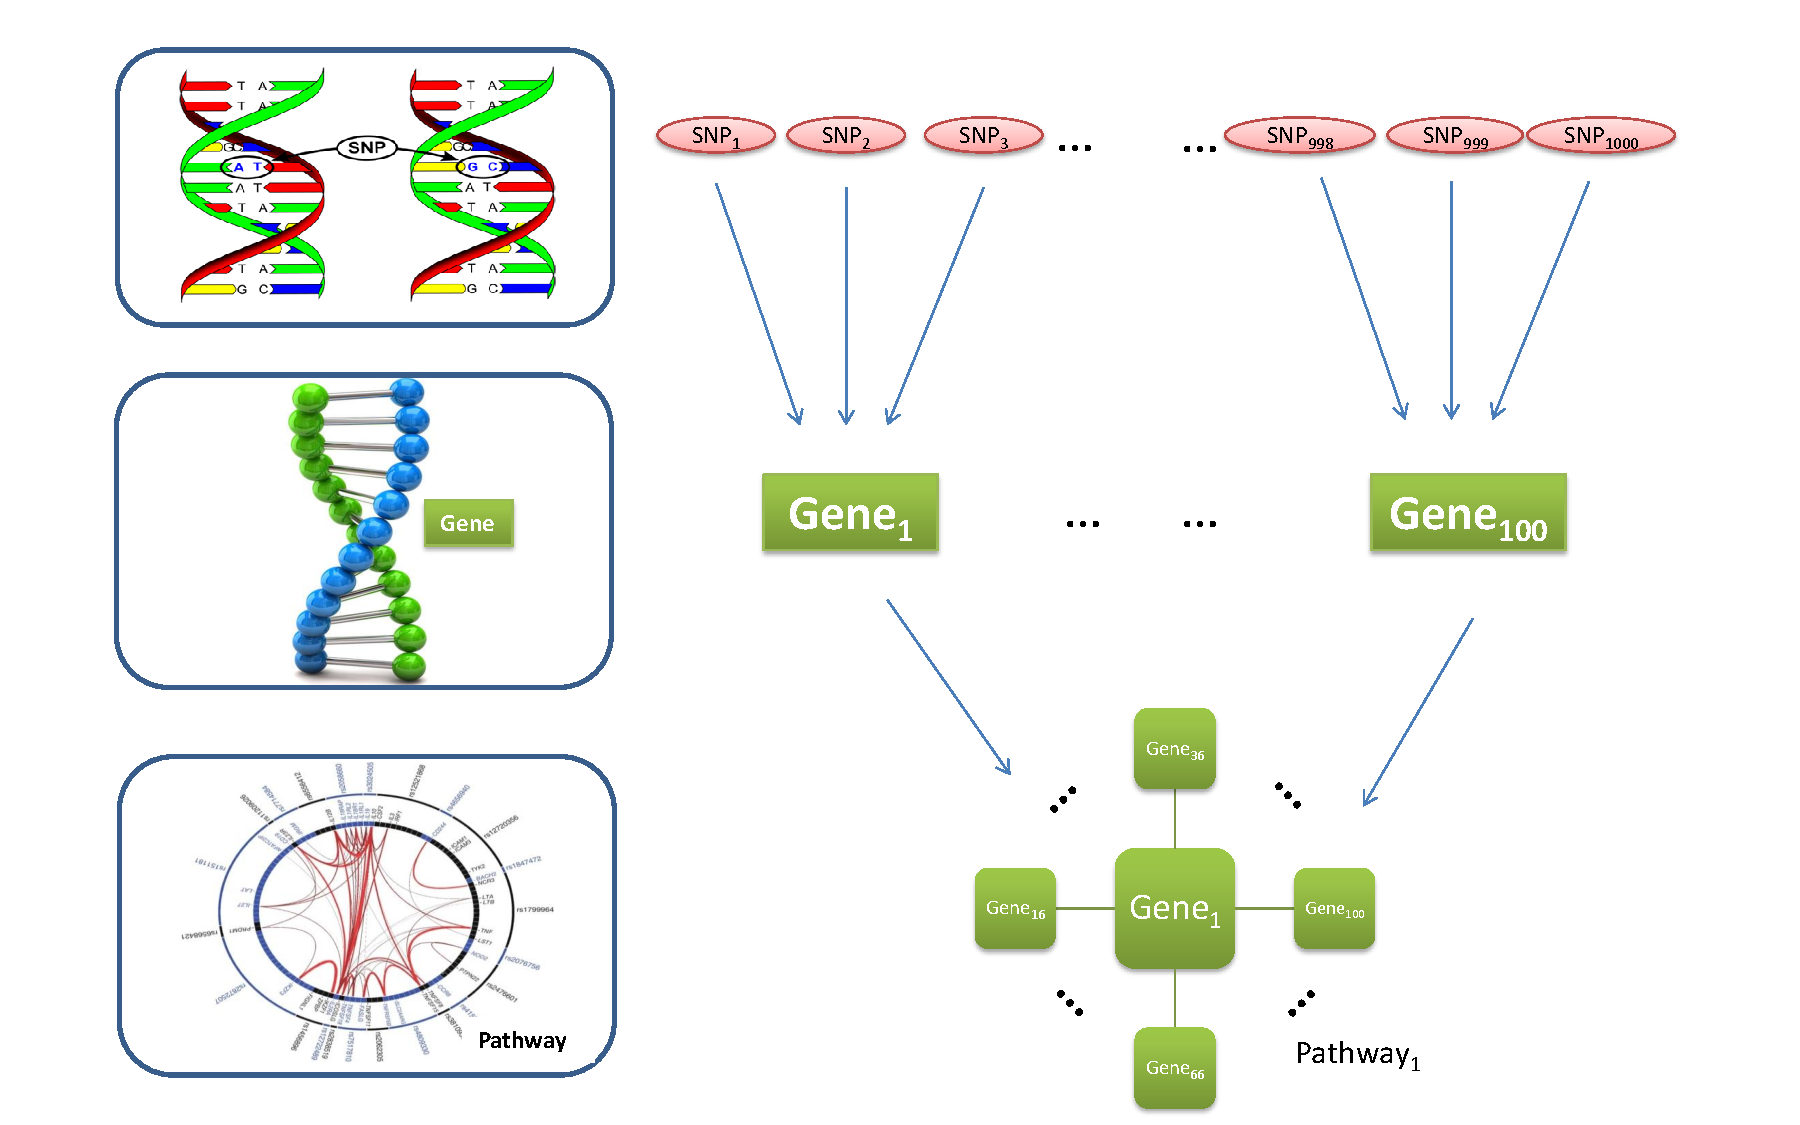
\includegraphics[width=1\textheight]{{{figure/Article2_SNPs_aggregation_flowchart}}}
%\vspace{-1cm}
\caption{\footnotesize Aggregation of SNPs in a Pathway}
\label{fig: Article2_SNPs_aggregation_flowchart}
\end{figure}



\framebreak
\scriptsize
A pathway analysis involves multiple genes (e.g. 20 as a typical number). As the genes within a pathway may contain different numbers of RVs, we need to modify the aSPU test to \textbf{adjust for various gene length} to avoid dominant influence from a large (or small) gene.\\\

Suppose we let the short notation $U_{g.}$ to represent $U_{.2}$ for the RVs $X_i$'part in the whole score vector, and $U_{g.} = (U_{g,1},U_{g,1},\ldots, U_{g,p_g})'$ is the score vector for gene $g$ with $p_g$ RVs of itself. Given a pathway (or gene set) S, the gene-specific SPU statistic is as follows:
\begin{equation}
T_ { SPU(\gamma ; g) } \propto || Ug.||_{\gamma} =  \left( \frac{  \sum_{j=1} ^ {p_g} |U_{g, j}| ^ { \gamma }  }{p_g} \right) ^ { 1 \over \gamma }
\end{equation}  
Then accordingly, the pathway-based SPU statistic is
\begin{equation}
T _ { Path-SPU(\gamma, \gamma2 ; S) } = \sum_{g \in S} ( T_ { SPU(\gamma ; g) } ) ^ {\gamma2}
\end{equation} 


\framebreak
The pathway-based aSPU statistic is thus
\begin{equation}
T _ { Path-aSPU(S) } = min_{\gamma, \gamma2} P _ { Path-SPU(\gamma, \gamma2 ; S) }
\end{equation}

We propose to use $\gamma 2 \in \Gamma 2 = \{1,2,4,8\}$. The $1,2,4,8$ will cover Sum-like test, SSU-like test, and two more tests preferring the sparse-causal-gene situation (e.g. only 2 or 3 genes are associated with traits in a pathway, say with 20 genes). 
}
 
%%%%%%%%%%%%%%%%%%%%%%
\subsubsection{ Data Simulation Methods}
\frame{
\frametitle{Table of Contents}
\small
\tableofcontents[currentsection,currentsubsection]
}
%3
\begin{frame}[allowframebreaks]
\frametitle{Simulation Methods}
\framesubtitle{Journal Article 2}
\small

\begin{itemize}
\item We simulated a pathway with 20 independent genes. Each gene $g$ contained $p_g$ SNPs with $p_g$ randomly draw from a uniform distribution $U(3,20)$; 5 of the 20 genes will be randomly selected to be causal, with each causal gene containing $U(1,3)$ causal SNPs. 
%The RVs within each gene will be simulated as before. The phenotype data in the simulation study will be the same as before.
\item The other parts of the simulation are the same as the article 1.
\end{itemize}

\framebreak
\textbf{Summary of parameter setup in simulation studies}
\footnotesize
\begin{itemize}
\item $h_j^2 = $ 0 or $h_j^2 = $ 0.001, 0.0025, 0.005, 0.0075 and 0.010
\item $\sigma_b = 7$
\item $\sigma_e = 27$
\item $k = 5$
\item 1000 replicates of simulated dataset
\item B = 1000
\item $\alpha = 0.05$
\item $\rho_y = 0.7$
\item $\rho_x = 0.8$
\item $R = AR(1)$
\item $Rw = I$
\item 0.05 $<$ MAF $<$ 0.4 for CVs; 0.001 $<$ MAF $<$ 0.01 for RVs
\item causal SNPs are excluded from testing for CVs but retained for RVs
\end{itemize}
\end{frame}


\subsubsection{Simulation Results}
\frame{
\frametitle{Table of Contents}
\small
\tableofcontents[currentsection,currentsubsection]
}
\begin{frame}[allowframebreaks]
\frametitle{Simulation Results}
\framesubtitle{Journal Article 2}
%\scriptsize
\begin{itemize}
\item \textbf{Simulation setting A}
%
\begin{itemize}
\item 0.05 $<$ MAF $<$ 0.4
\item $h_j^2 = 0$ 
\item $\alpha = 0.05$
\end{itemize}
%
\vspace{1cm}
%
\small
\begin{table}[ht]
%\resizebox{0.9\textwidth}{!}
%{
\centering
\begin{tabular}{rrrrrrrrrrr}
  \hline
 & pSSU & pSSUw & pScore & pSum & pUminP \\
  \hline
 & 0.037  & 0.042 & 0.025 & 0.049 & 0.050& \\
   \hline
\end{tabular}
\begin{tabular}{rrrrrrrrrrrr}
  \hline
 & LaSPUpath \\
  \hline
 & 0.053 \\
   \hline
\end{tabular}
%}
\caption{Empirical Type I Error Table in the simulation set-up A.}
\label{table:CV_typeIerror_pathway}
\end{table}

%-----------------------------------------------------------------%
\framebreak
\item \textbf{Simulation setting B}
%\begin{itemize}
%%\item 0.05 $<$ MAF $<$ 0.4
%\item $h_j^2 = $ 0.001, 0.0025, 0.005, 0.0075 and 0.010 
%%\item $\alpha = 0.05$
%\end{itemize}
\begin{figure}[H]
\centering
\vspace{-10pt}
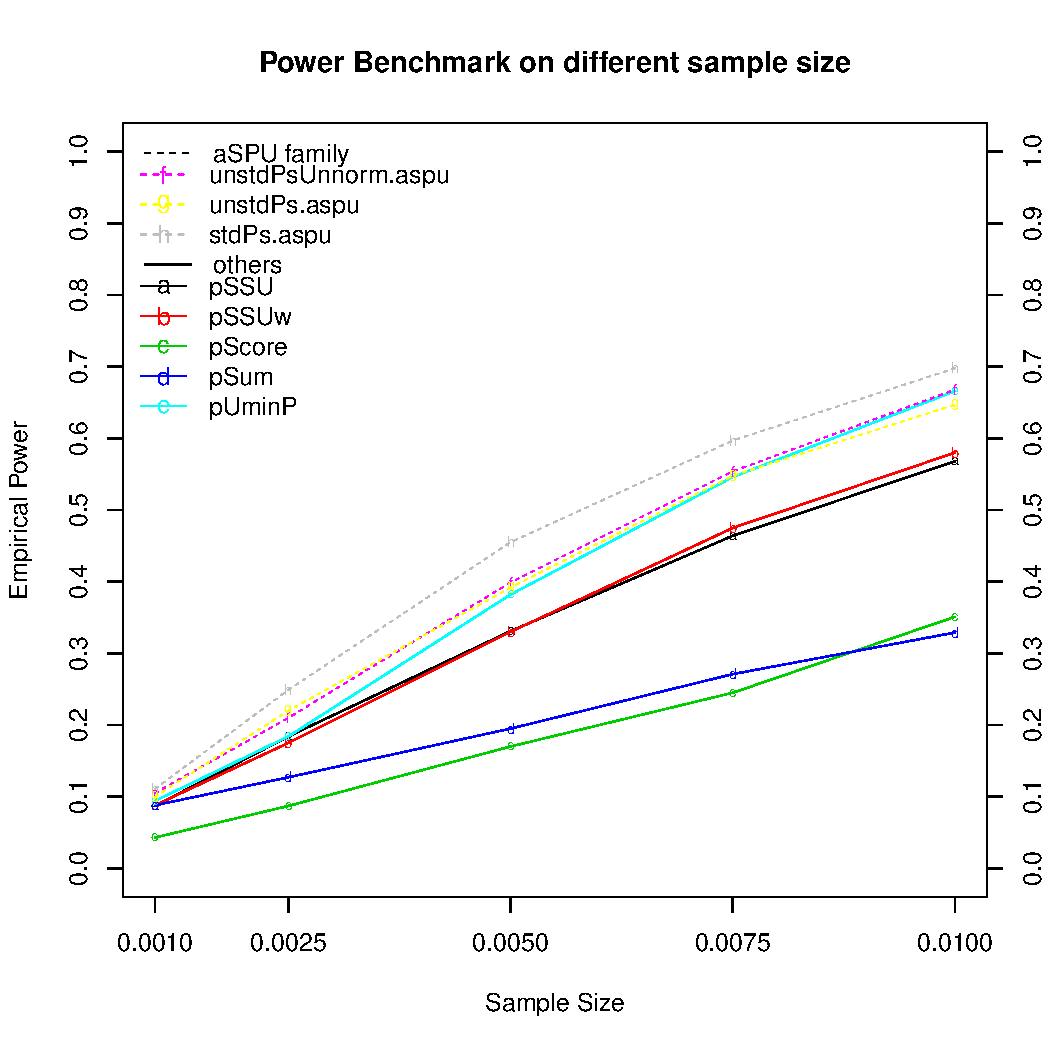
\includegraphics[height=0.7\textheight]{{{figure/PowerCurve_independenceWkCor_on_AR1data_RVsimulatedU_pathwayAnalysis}}}
\vspace{-10pt}
\caption{Empirical power benchmark under different heritability ($h^2$) in the simulation set-up B.}
\label{fig: PowerCurve_independenceWkCor_on_AR1data_h:vary_RVsimulatedU_pathway}
\end{figure}

\end{itemize}

\end{frame}

%-------------------------------------------------------------------------------------------------%
\subsubsection{Application to the ARIC Study}
\frame{
\frametitle{Table of Contents}
\small
\tableofcontents[currentsection,currentsubsection]
}
%%%%%
\begin{frame}[allowframebreaks]
\footnotesize
\frametitle{Application to the ARIC study}
\framesubtitle{Journal Article 2}
%------------------1---------------------%
\footnotesize
\textbf{Methods in data application}
\begin{itemize}
\item RV defined by MAF $<$ 0.05
\item Inclusion of only nonsynonymous and splice site variants
\item QC procedures as in \cite{Peloso2014}
\item Additive genetic model
\item Covariates include age, age$^2$, gender, BMI, time of measurement and top two PCs
\item obtain biological pathways from the KEGG database \cite{Ogata1999}
\item trim pathway to be of moderate size (between 10 and 500 genes)
\item Gene boundary defined in \cite{Peloso2014}
\item Significant: 0.05/197 = 0.00025; marginal significant: 1e-03
\end{itemize}

%\framebreak
%%------------------2---------------------%
%\textbf{\footnotesize Results in data application: compare longitudinal method with baseline method}
%\vspace{-10pt}
%\begin{figure}[b]
%\centering
%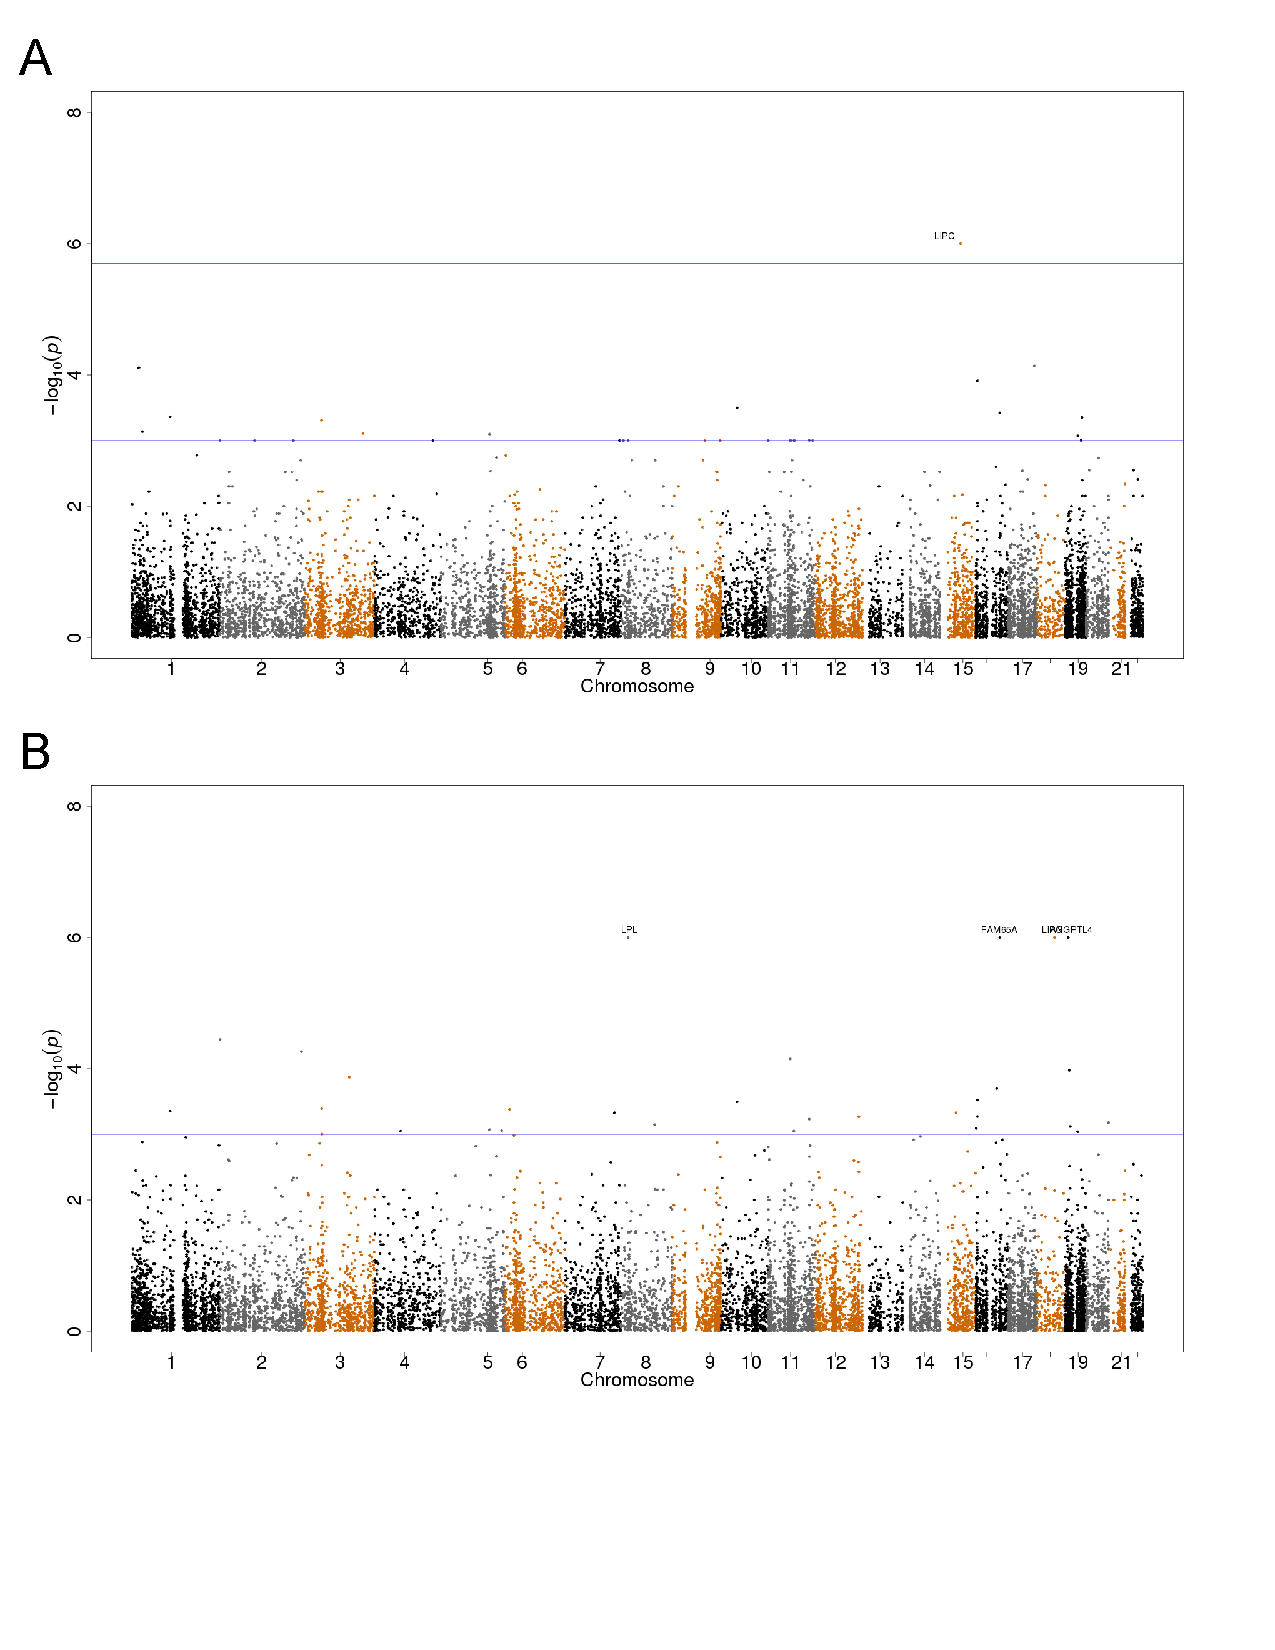
\includegraphics[height=0.76\textheight]{{{figure/compare_longi_LaSPU_exome_ARIC}}}
%\vspace{-1cm}
%\caption{\tiny Manhattan Plot Comparison between baseline study and longitudinal study by LaSPU test on the association between HDL-C and Rare Variants in the ARIC study. A. baseline study; B. longitudinal study using total four measurements.  }
%\label{fig: compare_longi_LaSPU_exome_ARIC}
%\end{figure}

\framebreak
%----------------------------------------%
\textbf{Results in data application: significant pathways}
\tiny
\ctable[
caption = {Results of the ARIC Data Application: KEGG Pathways with p Value $<$ 0.00025},
label = tab:table_pathway_based,
pos = ht,
width =  \textwidth,
center
%mincapwidth = \textwidth,
]{lcrrrr}{
  \tnote[a]{p Value of the gene $<$ 0.05}
}{
														    \toprule[1pt]
KEGG ID & Pathway Name & No. of Genes & No. of SNPs & p Value & Contributing Genes\tmark[a] \ML
hsa00561 & Glycerolipid metabolism & 44 & 311 & 1.00E-06 & \tiny \shortstack{ \textit{LPL,LIPG,LIPC,}\\\textit{DGKQ,PPAP2A,PNLIPRP3}} \\
hsa03320 & PPAR signaling pathway & 55 & 465 & 1.00E-06 & \tiny \shortstack{ \textit{LPL,ANGPTL4,NR1H3,}\\\textit{CD36,APOA1}} \\
hsa05010 & Alzheimers disease & 98 & 747 & 1.00E-06 & \tiny \shortstack{ \textit{LPL,APOE,BID,PLCB3,NDUFS8,}\\
\textit{NDUFS3,NDUFB6,RYR3,NCSTN}} \LL
}
\end{frame}



%-------------------------------------------------------------------------------------------------%
%%%%%%%%%%%%%%%%%%%%%%%%%%%%%%%%%%%
%%%%%%%%%%%%%%%%%%%%%%%%%%%%%%%%%%%
\subsubsection{Discussion}
%%%%%%%%%%%%%%%%%%%%%%%%%%%%%%%%%%%
%%%%%%%%%%%%%%%%%%%%%%%%%%%%%%%%%%%
\frame{
\frametitle{Table of Contents}
\small
\tableofcontents[currentsection,currentsubsection]
}
\begin{frame}[allowframebreaks]
\footnotesize
\frametitle{Discussion}
\framesubtitle{Journal Article 1}
%------------------1---------------------%
\begin{itemize}
\item LaSPUpath could efficiently use the longitudinal information to increase testing power
\item LaSPU could efficiently use the biological information (such as pathway) to increase the testing power
\item LaSPUpath could adaptively select the best test and achieve a greater power
\item LaSPUpath identified three pathways significantly associated with HDL-C. The annotated functions of the pathways closely relate HDL-C, either as the regulator of lipids (including HDL-C) and/or lead to the lipid-related diseases like Hyperlipoproteinemia and Alzheimer's disease.
\item LaSPUpath could be used in more extended gene-set based testings, for example, annotations of functional variation available in RegulomeDB\cite{Boyle2012} and epigenome activities collected in The Human Epigenome Atlas (http://www.genboree.org/epigenomeatlas/).
\end{itemize}
\end{frame}





%%%%%%%%%%%%%%%%%%%%%%%%%%%%%%%%%%%%%%%%%%%%%%%%%%%
%%%%%%%%%%%%%%%%%%%%%%%%%%%%%%%%%%%%%%%%%%%%
%%%%%%%%%%%%%%%%%%%%%%%%%%%%%%%%%%%%%%%%%%%%%%%%%%%
\subsection{Journal Article 3: LaSPU: a suite of powerful data-adaptive SNP-set and ...}
%%%%%%%%%%%%%%%%%%%%%%%%%%%%%%%%%%%%%%%%%%%%%%%%%%%
%%%%%%%%%%%%%%%%%%%%%%%%%%%%%%%%%%%%%%%%%%%%
%%%%%%%%%%%%%%%%%%%%%%%%%%%%%%%%%%%%%%%%%%%%%%%%%%%
\frame{
\frametitle{Table of Contents}
\small
\tableofcontents[currentsection,currentsubsection]
}

%%%%%%%%%%%%%%%%%%%%%%%
%%%%%%%%%%%%%%%%%%%%%%%
%1
\frame{
\frametitle{Journal Article 3}
%\framesubtitle{Aim 1a}
\small
\textbf{Title of Journal Article}\\
LaSPU: a suite of powerful data-adaptive SNP-set and pathway-based association testing
tools for longitudinal traits.\\\

\textbf{Name of Journal Proposed for Article Submission}\\
Bioinformatics (as application note)
}
%%%%%%%%%%%%%%%%%%%%%%%
%%%%%%%%%%%%%%%%%%%%%%%
%\subsubsection{Features and Workflow}
%\frame{
%\frametitle{Table of Contents}
%\small
%\tableofcontents[currentsection,currentsubsection]
%}
%2----------------------------------------%
\frame{
\frametitle{Features}
\framesubtitle{Journal Article 3}
\begin{itemize}
\item implement the LaSPU method
\item compatible with Unix-like system
\item command line operated program
\item optimized and possess flexible parallel computing schema
\item user-friendly manual and examples
\end{itemize}
}
%-----------------------------------%
\frame{
\frametitle{Workflow}
\framesubtitle{Journal Article 3}
\begin{figure}[H]
\centering
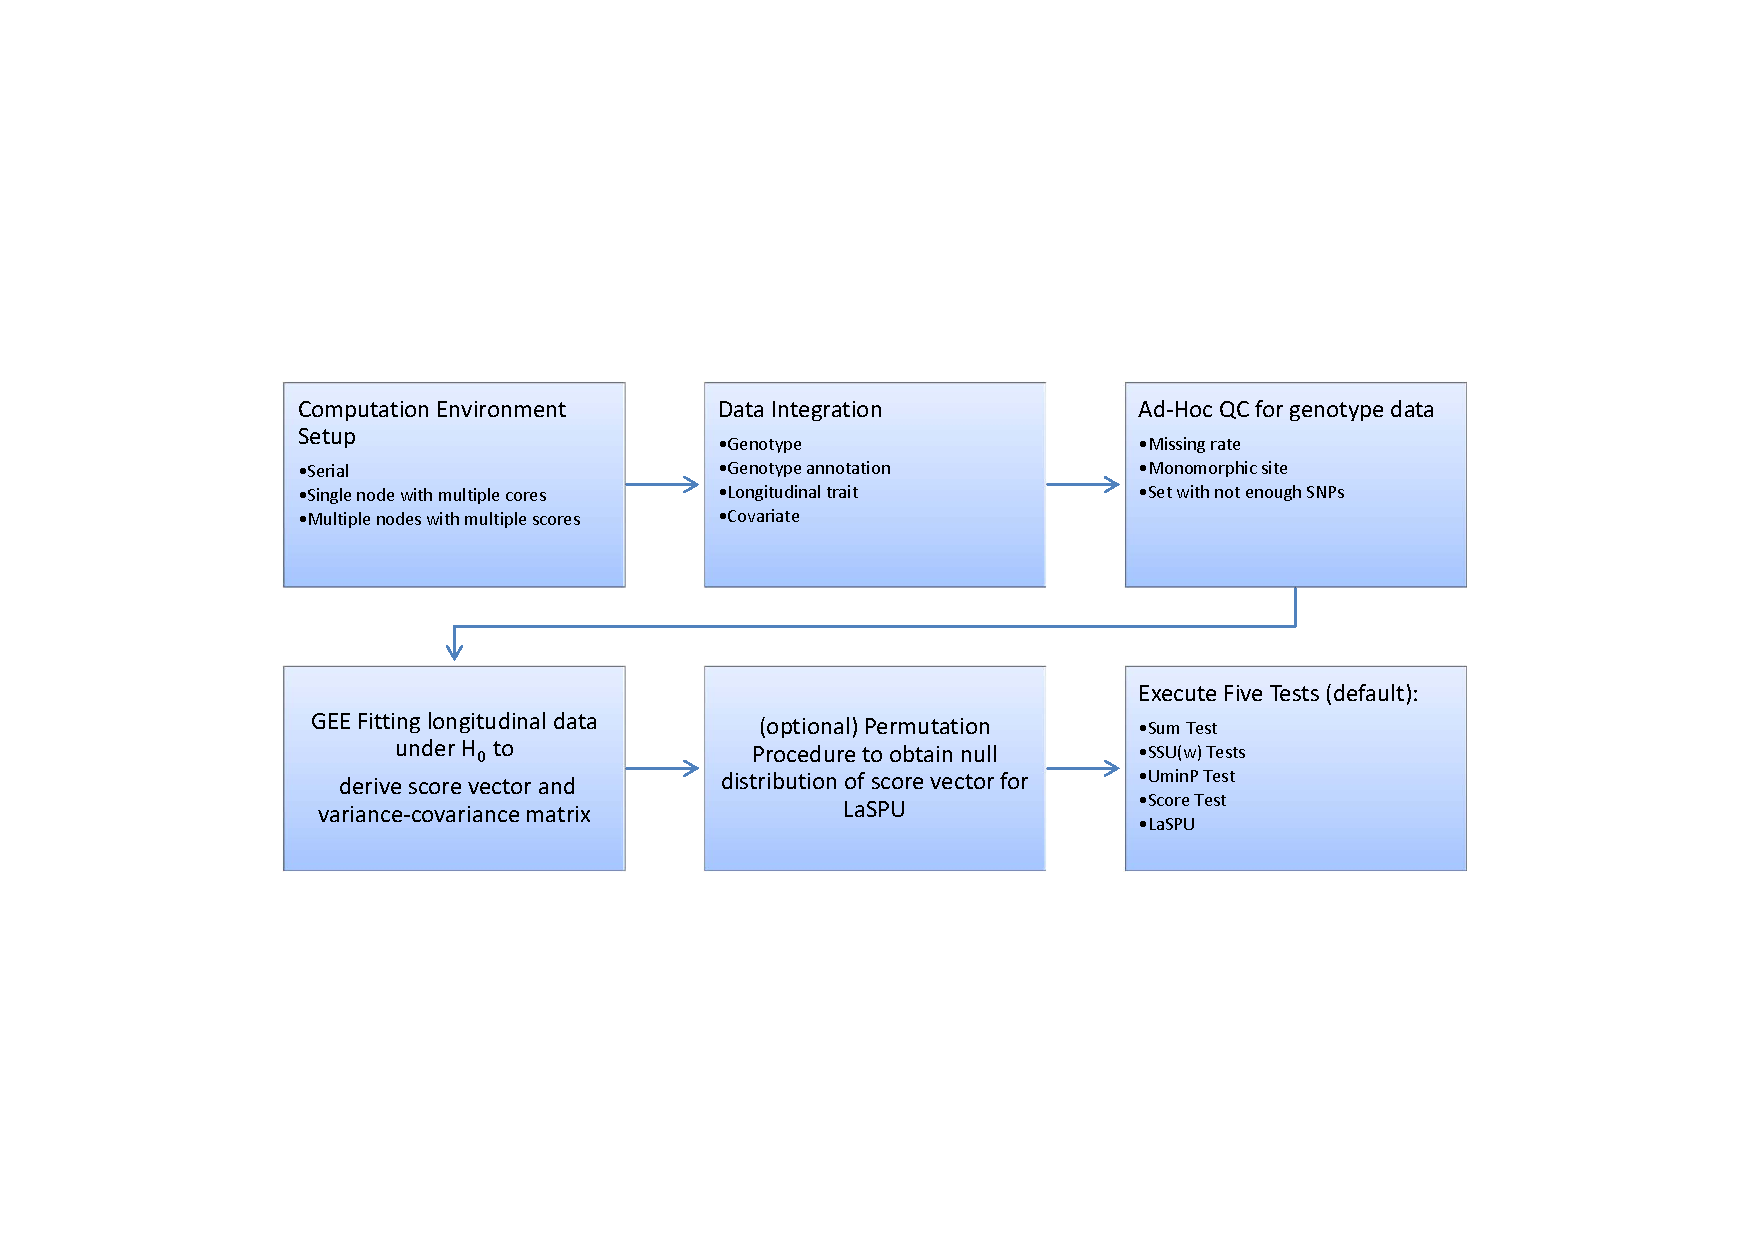
\includegraphics[width=0.9\textwidth]{{{figure/Article3_workflow}}}
\vspace{-10pt}
\caption{\footnotesize LaSPU Workflow Chart.}
\label{fig: LaSPU_workflow}
\end{figure}
}
%-----------------------------------%
\frame{
\frametitle{Result}
\framesubtitle{Journal Article 3}
Free downloadable at https://github.com/xyy2006/LaSPU
}
%%%%%%%%%%%%%%%%%%%%%%%
%%%%%%%%%%%%%%%%%%%%%%%


%%%%%%%%%%%%%%%%%%%%%%%%%%%%%%%%%%%%%%%%%%
%%%%%%%%%%%%%%%%%%%%%%%%%%%%%%%%%%%%%%%%%%
%%%%%%%%%%%%%%%%%%%%%%%%%%%%%%%%%%%%%%%%%  
%%%%%%%%%%%%%%%%%%%%%%%%%%%%%%%%%%%%%%%%%%%%%%%%%%%%%%%%%%%%
\section{Conclusion and Futurework}\label{sec:data}
%%%%%%%%%%%%%%%%%%%%%%%%%%%%%%%%%%%%%%%%%%%%%%%%%%%%%%%%%%%%
%\subsection{Real Data Introduction}\label{sec:data-intro}
\frame{
\frametitle{Table of Contents}
\small
\tableofcontents[currentsection,currentsubsection]
}

\frame{
\scriptsize
\frametitle{Conclusion}
\begin{itemize}
\item The development of the LaSPU method
\item The development of the LaSPUpath method
\item The development of the "LaSPU" software package

\end{itemize}

}



%%%%%%%%%%%%%%%%%%%%%%%%%%%%%%%%%%%%%%%%%%
%%%%%%%%%%%%%%%%%%%%%%%%%%%%%%%%%%%%%%%%%%
%%%%%%%%%%%%%%%%%%%%%%%%%%%%%%%%%%%%%%%%%  
%%%%%%%%%%%%%%%%%%%%%%%%%%%%%%%%%%%%%%%%%%%%%%%%%%%%%%%%%%%%
\section{Acknowledgement}\label{sec:acknow}
%%%%%%%%%%%%%%%%%%%%%%%%%%%%%%%%%%%%%%%%%%%%%%%%%%%%%%%%%%%%
%\subsection{Real Data Introduction}\label{sec:data-intro}
\frame{
\frametitle{Table of Contents}
\small
\tableofcontents[currentsection,currentsubsection]
}

% acknowledgement frame  
\frame{
\frametitle{Acknowledgement}
\textbf{Advisers:}\\
\begin{itemize}
\item Peng Wei, Ph.D, Associate Professor, Division of Biostatistics, School of Public Health, University of Texas
\item Wei Pan, Ph.D, Professor, Division of Biostatistics, School of Public Health, University of Minnesota
\end{itemize}

\textbf{Supporting Grant:}\\
Title: Association Analysis of Rare Variants with Sequencing Data\\ 
Funding Source: NIH/NHLBI (1R01HL116720) \\
Total cost: $\$1,043,901$ \\
}


%%%%%%%%%%%%%%%%%%%%%%%%%%%%%%
% acknowledgement frame  
\frame{
\frametitle{Thanks to Audience}
%\begin{figure}
%        \centering
%        \begin{subfigure}[b]{0.4\textwidth}
%                
\includegraphics[width=\textwidth]{figure/QA_amazon}
%                %\caption{A gull}
%                %\label{fig:gull}
%        \end{subfigure}%
%        ~ %add desired spacing between images, e. g. ~, \quad, \qquad, \hfill etc.
%          %(or a blank line to force the subfigure onto a new line)
%        \begin{subfigure}[b]{0.4\textwidth}
%                
\includegraphics[width=\textwidth]{figure/QA1}
%                %\caption{A tiger}
%                %\label{fig:tiger}
%        \end{subfigure}
%        %\caption{Pictures of animals}\label{fig:animals}
%\end{figure}

 \begin{figure}
        \centering
        \begin{minipage}{.5\textwidth}
            \centering
            \includegraphics[width=.6\linewidth]{figure/fred-hutchinson-cancer-research-center2}
            %\caption{A subfigure}
        \end{minipage}%
        \begin{minipage}{.5\textwidth}
            \centering
            
\includegraphics[width=.6\linewidth]{figure/QA1}
            %\caption{A subfigure}
        \end{minipage}
        %\caption{Thank you for your participation!}
    \end{figure}
    \centering
    Thank you for your participation!

}

\section{References}
%\frame{
%\frametitle{References}
%\begin{enumerate}
%\item Elizabeth R. Brown, {\em Introduction to Regression Models}
%\item Nicholas Christian, {\em Statistical Computing in R}
%\item Langsrud, $\phi$. (2003), ANOVA for Unbalanced Data: Use Type II Instead of Type III Sums of Squares, {\em Statistics and Computing}, 13, 163-167.
%\end{enumerate}
 
\begin{frame}[allowframebreaks]
\tiny
        \frametitle{References}
        \bibliographystyle{amsalpha}
        \bibliography{../proposal}
\end{frame}
%}
  
\end{document}